% Options for packages loaded elsewhere
\PassOptionsToPackage{unicode}{hyperref}
\PassOptionsToPackage{hyphens}{url}
%
\documentclass[
]{book}
\usepackage{amsmath,amssymb}
\usepackage{lmodern}
\usepackage{ifxetex,ifluatex}
\ifnum 0\ifxetex 1\fi\ifluatex 1\fi=0 % if pdftex
  \usepackage[T1]{fontenc}
  \usepackage[utf8]{inputenc}
  \usepackage{textcomp} % provide euro and other symbols
\else % if luatex or xetex
  \usepackage{unicode-math}
  \defaultfontfeatures{Scale=MatchLowercase}
  \defaultfontfeatures[\rmfamily]{Ligatures=TeX,Scale=1}
\fi
% Use upquote if available, for straight quotes in verbatim environments
\IfFileExists{upquote.sty}{\usepackage{upquote}}{}
\IfFileExists{microtype.sty}{% use microtype if available
  \usepackage[]{microtype}
  \UseMicrotypeSet[protrusion]{basicmath} % disable protrusion for tt fonts
}{}
\makeatletter
\@ifundefined{KOMAClassName}{% if non-KOMA class
  \IfFileExists{parskip.sty}{%
    \usepackage{parskip}
  }{% else
    \setlength{\parindent}{0pt}
    \setlength{\parskip}{6pt plus 2pt minus 1pt}}
}{% if KOMA class
  \KOMAoptions{parskip=half}}
\makeatother
\usepackage{xcolor}
\IfFileExists{xurl.sty}{\usepackage{xurl}}{} % add URL line breaks if available
\IfFileExists{bookmark.sty}{\usepackage{bookmark}}{\usepackage{hyperref}}
\hypersetup{
  pdftitle={STAT 454 Bayesian Statistics: Short term COVID-19 prediction model using monthly incidence data},
  pdfauthor={Raymond Gu, Zefan Qian},
  hidelinks,
  pdfcreator={LaTeX via pandoc}}
\urlstyle{same} % disable monospaced font for URLs
\usepackage{color}
\usepackage{fancyvrb}
\newcommand{\VerbBar}{|}
\newcommand{\VERB}{\Verb[commandchars=\\\{\}]}
\DefineVerbatimEnvironment{Highlighting}{Verbatim}{commandchars=\\\{\}}
% Add ',fontsize=\small' for more characters per line
\usepackage{framed}
\definecolor{shadecolor}{RGB}{248,248,248}
\newenvironment{Shaded}{\begin{snugshade}}{\end{snugshade}}
\newcommand{\AlertTok}[1]{\textcolor[rgb]{0.94,0.16,0.16}{#1}}
\newcommand{\AnnotationTok}[1]{\textcolor[rgb]{0.56,0.35,0.01}{\textbf{\textit{#1}}}}
\newcommand{\AttributeTok}[1]{\textcolor[rgb]{0.77,0.63,0.00}{#1}}
\newcommand{\BaseNTok}[1]{\textcolor[rgb]{0.00,0.00,0.81}{#1}}
\newcommand{\BuiltInTok}[1]{#1}
\newcommand{\CharTok}[1]{\textcolor[rgb]{0.31,0.60,0.02}{#1}}
\newcommand{\CommentTok}[1]{\textcolor[rgb]{0.56,0.35,0.01}{\textit{#1}}}
\newcommand{\CommentVarTok}[1]{\textcolor[rgb]{0.56,0.35,0.01}{\textbf{\textit{#1}}}}
\newcommand{\ConstantTok}[1]{\textcolor[rgb]{0.00,0.00,0.00}{#1}}
\newcommand{\ControlFlowTok}[1]{\textcolor[rgb]{0.13,0.29,0.53}{\textbf{#1}}}
\newcommand{\DataTypeTok}[1]{\textcolor[rgb]{0.13,0.29,0.53}{#1}}
\newcommand{\DecValTok}[1]{\textcolor[rgb]{0.00,0.00,0.81}{#1}}
\newcommand{\DocumentationTok}[1]{\textcolor[rgb]{0.56,0.35,0.01}{\textbf{\textit{#1}}}}
\newcommand{\ErrorTok}[1]{\textcolor[rgb]{0.64,0.00,0.00}{\textbf{#1}}}
\newcommand{\ExtensionTok}[1]{#1}
\newcommand{\FloatTok}[1]{\textcolor[rgb]{0.00,0.00,0.81}{#1}}
\newcommand{\FunctionTok}[1]{\textcolor[rgb]{0.00,0.00,0.00}{#1}}
\newcommand{\ImportTok}[1]{#1}
\newcommand{\InformationTok}[1]{\textcolor[rgb]{0.56,0.35,0.01}{\textbf{\textit{#1}}}}
\newcommand{\KeywordTok}[1]{\textcolor[rgb]{0.13,0.29,0.53}{\textbf{#1}}}
\newcommand{\NormalTok}[1]{#1}
\newcommand{\OperatorTok}[1]{\textcolor[rgb]{0.81,0.36,0.00}{\textbf{#1}}}
\newcommand{\OtherTok}[1]{\textcolor[rgb]{0.56,0.35,0.01}{#1}}
\newcommand{\PreprocessorTok}[1]{\textcolor[rgb]{0.56,0.35,0.01}{\textit{#1}}}
\newcommand{\RegionMarkerTok}[1]{#1}
\newcommand{\SpecialCharTok}[1]{\textcolor[rgb]{0.00,0.00,0.00}{#1}}
\newcommand{\SpecialStringTok}[1]{\textcolor[rgb]{0.31,0.60,0.02}{#1}}
\newcommand{\StringTok}[1]{\textcolor[rgb]{0.31,0.60,0.02}{#1}}
\newcommand{\VariableTok}[1]{\textcolor[rgb]{0.00,0.00,0.00}{#1}}
\newcommand{\VerbatimStringTok}[1]{\textcolor[rgb]{0.31,0.60,0.02}{#1}}
\newcommand{\WarningTok}[1]{\textcolor[rgb]{0.56,0.35,0.01}{\textbf{\textit{#1}}}}
\usepackage{longtable,booktabs,array}
\usepackage{calc} % for calculating minipage widths
% Correct order of tables after \paragraph or \subparagraph
\usepackage{etoolbox}
\makeatletter
\patchcmd\longtable{\par}{\if@noskipsec\mbox{}\fi\par}{}{}
\makeatother
% Allow footnotes in longtable head/foot
\IfFileExists{footnotehyper.sty}{\usepackage{footnotehyper}}{\usepackage{footnote}}
\makesavenoteenv{longtable}
\usepackage{graphicx}
\makeatletter
\def\maxwidth{\ifdim\Gin@nat@width>\linewidth\linewidth\else\Gin@nat@width\fi}
\def\maxheight{\ifdim\Gin@nat@height>\textheight\textheight\else\Gin@nat@height\fi}
\makeatother
% Scale images if necessary, so that they will not overflow the page
% margins by default, and it is still possible to overwrite the defaults
% using explicit options in \includegraphics[width, height, ...]{}
\setkeys{Gin}{width=\maxwidth,height=\maxheight,keepaspectratio}
% Set default figure placement to htbp
\makeatletter
\def\fps@figure{htbp}
\makeatother
\setlength{\emergencystretch}{3em} % prevent overfull lines
\providecommand{\tightlist}{%
  \setlength{\itemsep}{0pt}\setlength{\parskip}{0pt}}
\setcounter{secnumdepth}{5}
\usepackage{booktabs}
\usepackage{amsthm}
\makeatletter
\def\thm@space@setup{%
  \thm@preskip=8pt plus 2pt minus 4pt
  \thm@postskip=\thm@preskip
}
\makeatother
\ifluatex
  \usepackage{selnolig}  % disable illegal ligatures
\fi
\usepackage[]{natbib}
\bibliographystyle{apalike}

\title{STAT 454 Bayesian Statistics: Short term COVID-19 prediction model using monthly incidence data}
\author{Raymond Gu, Zefan Qian}
\date{2021-12-03}

\begin{document}
\maketitle

{
\setcounter{tocdepth}{1}
\tableofcontents
}
\hypertarget{preface}{%
\chapter{Preface}\label{preface}}

This is the bookdown of Raymond and Zefan's STAT 455 Bayesian Statistics Project.

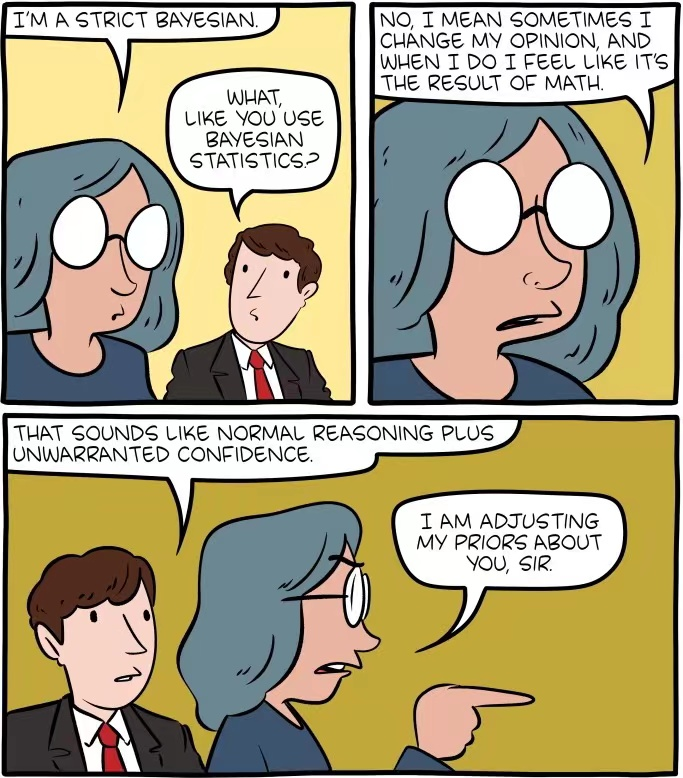
\includegraphics{preface_comic.jpg}

Credit to \href{smbc-comics.com}{SMBC}.

\hypertarget{intro}{%
\chapter{Motivation}\label{intro}}

First identified in Botswana and South Africa, this new iteration of the coronavirus Omicron has prompted concern among scientists and public health officials because of an unusually high number of mutations that have the potential to make the virus more transmissible and less susceptible to existing vaccines. Hence a big question for humanity is: when will it end or at least not affect people's lives? In our report, we aim to investigate how factors such as state and time can help us predict future outbreaks. The investigation potentially can help people decide to what places and at what time are they safe to travel if they have to.

\hypertarget{data}{%
\chapter{Data}\label{data}}

\hypertarget{data-source}{%
\section{Data Source}\label{data-source}}

Our data was collected from the New York Times, which is an American daily newspaper based in New York City with a worldwide readership. The data is held on New York Times COVID-19 Github repository. The data is updating itself every day by the end of day and the latest update will be today, when we are doing our analysis. This dataset includes cumulative cases and deaths reported in each state across the U.S., including U.S. territories and the District of Columbia, since the beginning of the pandemic beginning in Jan 21, 2021.

Website for our data source: \url{https://raw.githubusercontent.com/nytimes/covid-19-data/master/us-states.csv}

\hypertarget{data-dictionary}{%
\section{Data Dictionary}\label{data-dictionary}}

\begin{longtable}[]{@{}ll@{}}
\toprule
Variable Name & Description \\
\midrule
\endhead
date & Date \\
state & Name of State \\
fips & First Two Digits of ZipCode of the State \\
cases & Number of Cumulative Cases \\
deaths & Number of Cumulative Deaths \\
\bottomrule
\end{longtable}

\hypertarget{data-cleaning}{%
\chapter{Data Cleaning}\label{data-cleaning}}

\begin{Shaded}
\begin{Highlighting}[]
\CommentTok{\#load packages}
\FunctionTok{library}\NormalTok{(bayesrules)}
\FunctionTok{library}\NormalTok{(tidyverse)}
\FunctionTok{library}\NormalTok{(janitor)}
\FunctionTok{library}\NormalTok{(rstanarm)}
\FunctionTok{library}\NormalTok{(bayesplot)}
\FunctionTok{library}\NormalTok{(tidybayes)}
\FunctionTok{library}\NormalTok{(broom.mixed)}
\FunctionTok{library}\NormalTok{(modelr)}
\FunctionTok{library}\NormalTok{(e1071)}
\FunctionTok{library}\NormalTok{(forcats)}
\FunctionTok{library}\NormalTok{(ggExtra)}
\FunctionTok{library}\NormalTok{(ggpubr)}
\FunctionTok{library}\NormalTok{(ggridges)}
\FunctionTok{library}\NormalTok{(devtools)}
\FunctionTok{library}\NormalTok{(zoo)}
\FunctionTok{library}\NormalTok{(DT)}
\FunctionTok{library}\NormalTok{(dplyr)}
\FunctionTok{library}\NormalTok{(plyr)}
\end{Highlighting}
\end{Shaded}

\hypertarget{load-data}{%
\section{Load Data}\label{load-data}}

\begin{Shaded}
\begin{Highlighting}[]
\CommentTok{\#load data}
\NormalTok{covid19 }\OtherTok{\textless{}{-}} \FunctionTok{read\_csv}\NormalTok{(}\FunctionTok{url}\NormalTok{(}\StringTok{"https://raw.githubusercontent.com/nytimes/covid{-}19{-}data/master/us{-}states.csv"}\NormalTok{))}
\NormalTok{newdata }\OtherTok{\textless{}{-}} \FunctionTok{read.csv}\NormalTok{(}\StringTok{"C:/Users/qianz/Desktop/Macalester/Junior 1st semester/STAT 454/COVID{-}bookdown/bookdown{-}demo{-}main/prediction\_newdata.csv"}\NormalTok{)}
\end{Highlighting}
\end{Shaded}

\hypertarget{generate-monthly-incident-data}{%
\section{Generate Monthly Incident Data}\label{generate-monthly-incident-data}}

\begin{Shaded}
\begin{Highlighting}[]
\NormalTok{covid19\_filter }\OtherTok{\textless{}{-}}\NormalTok{ covid19 }\SpecialCharTok{\%\textgreater{}\%}
\NormalTok{  dplyr}\SpecialCharTok{::}\FunctionTok{group\_by}\NormalTok{(state) }\SpecialCharTok{\%\textgreater{}\%}
\NormalTok{  dplyr}\SpecialCharTok{::}\FunctionTok{mutate}\NormalTok{(}\AttributeTok{lag1 =} \FunctionTok{lag}\NormalTok{(cases, }\AttributeTok{n =} \DecValTok{1}\NormalTok{)) }

\NormalTok{covid19\_filter}\SpecialCharTok{$}\NormalTok{lag1 }\OtherTok{\textless{}{-}}\NormalTok{ covid19\_filter}\SpecialCharTok{$}\NormalTok{lag1 }\SpecialCharTok{\%\textgreater{}\%} 
  \FunctionTok{replace\_na}\NormalTok{(}\DecValTok{0}\NormalTok{)}

\NormalTok{covid19\_filter }\OtherTok{\textless{}{-}}\NormalTok{ covid19\_filter }\SpecialCharTok{\%\textgreater{}\%} \FunctionTok{mutate}\NormalTok{(}\AttributeTok{case\_new =}\NormalTok{ cases }\SpecialCharTok{{-}}\NormalTok{ lag1) }
\end{Highlighting}
\end{Shaded}

\hypertarget{generate-time-variables}{%
\section{Generate Time Variables}\label{generate-time-variables}}

\begin{Shaded}
\begin{Highlighting}[]
\NormalTok{covid19\_month }\OtherTok{\textless{}{-}}\NormalTok{ covid19\_filter }\SpecialCharTok{\%\textgreater{}\%}
\NormalTok{  dplyr}\SpecialCharTok{::}\FunctionTok{mutate}\NormalTok{(}\AttributeTok{year =}\NormalTok{ lubridate}\SpecialCharTok{::}\FunctionTok{year}\NormalTok{(date), }
                \AttributeTok{month =}\NormalTok{ lubridate}\SpecialCharTok{::}\FunctionTok{month}\NormalTok{(date), }
                \AttributeTok{day =}\NormalTok{ lubridate}\SpecialCharTok{::}\FunctionTok{day}\NormalTok{(date)) }\SpecialCharTok{\%\textgreater{}\%}
\NormalTok{  dplyr}\SpecialCharTok{::}\FunctionTok{group\_by}\NormalTok{(state, year, month) }\SpecialCharTok{\%\textgreater{}\%}
\NormalTok{  dplyr}\SpecialCharTok{::}\FunctionTok{summarize}\NormalTok{(}\AttributeTok{cases =} \FunctionTok{sum}\NormalTok{(case\_new)) }

\NormalTok{covid19\_month}\SpecialCharTok{$}\NormalTok{Date }\OtherTok{\textless{}{-}} \FunctionTok{as.yearmon}\NormalTok{(}\FunctionTok{paste}\NormalTok{(covid19\_month}\SpecialCharTok{$}\NormalTok{year, covid19\_month}\SpecialCharTok{$}\NormalTok{month), }\StringTok{"\%Y \%m"}\NormalTok{)}
\end{Highlighting}
\end{Shaded}

\hypertarget{remove-incomplete-monthly-data}{%
\section{Remove Incomplete Monthly Data}\label{remove-incomplete-monthly-data}}

\begin{Shaded}
\begin{Highlighting}[]
\NormalTok{covid19\_month }\OtherTok{\textless{}{-}}\NormalTok{ covid19\_month }\SpecialCharTok{\%\textgreater{}\%}
  \FunctionTok{filter}\NormalTok{(}\SpecialCharTok{!}\NormalTok{(year }\SpecialCharTok{==} \DecValTok{2021} \SpecialCharTok{\&}\NormalTok{ month }\SpecialCharTok{==} \DecValTok{12}\NormalTok{))}
\end{Highlighting}
\end{Shaded}

\hypertarget{generate-lag-in-time-series}{%
\section{Generate Lag in Time-Series}\label{generate-lag-in-time-series}}

\begin{Shaded}
\begin{Highlighting}[]
\NormalTok{covid19\_month }\OtherTok{\textless{}{-}}\NormalTok{ covid19\_month }\SpecialCharTok{\%\textgreater{}\%}
\NormalTok{  dplyr}\SpecialCharTok{::}\FunctionTok{group\_by}\NormalTok{(state) }\SpecialCharTok{\%\textgreater{}\%}
\NormalTok{  dplyr}\SpecialCharTok{::}\FunctionTok{mutate}\NormalTok{(}\AttributeTok{lag1 =} \FunctionTok{lag}\NormalTok{(cases, }\AttributeTok{n =} \DecValTok{1}\NormalTok{)) }

\NormalTok{covid19\_month}\SpecialCharTok{$}\NormalTok{lag1 }\OtherTok{\textless{}{-}}\NormalTok{ covid19\_month}\SpecialCharTok{$}\NormalTok{lag1 }\SpecialCharTok{\%\textgreater{}\%} 
  \FunctionTok{replace\_na}\NormalTok{(}\DecValTok{0}\NormalTok{)}

\NormalTok{covid19\_month }\OtherTok{\textless{}{-}}\NormalTok{ covid19\_month }\SpecialCharTok{\%\textgreater{}\%}
\NormalTok{  dplyr}\SpecialCharTok{::}\FunctionTok{group\_by}\NormalTok{(state) }\SpecialCharTok{\%\textgreater{}\%}
  \FunctionTok{mutate}\NormalTok{(}\AttributeTok{lag3 =} \FunctionTok{lag}\NormalTok{(cases, }\AttributeTok{n =} \DecValTok{3}\NormalTok{)) }

\NormalTok{covid19\_month}\SpecialCharTok{$}\NormalTok{lag3 }\OtherTok{\textless{}{-}}\NormalTok{ covid19\_month}\SpecialCharTok{$}\NormalTok{lag3 }\SpecialCharTok{\%\textgreater{}\%} 
  \FunctionTok{replace\_na}\NormalTok{(}\DecValTok{0}\NormalTok{)}

\NormalTok{covid19\_month }\OtherTok{\textless{}{-}}\NormalTok{ covid19\_month }\SpecialCharTok{\%\textgreater{}\%}
\NormalTok{  dplyr}\SpecialCharTok{::}\FunctionTok{group\_by}\NormalTok{(state) }\SpecialCharTok{\%\textgreater{}\%}
  \FunctionTok{mutate}\NormalTok{(}\AttributeTok{lag6 =} \FunctionTok{lag}\NormalTok{(cases, }\AttributeTok{n =} \DecValTok{6}\NormalTok{)) }

\NormalTok{covid19\_month}\SpecialCharTok{$}\NormalTok{lag6 }\OtherTok{\textless{}{-}}\NormalTok{ covid19\_month}\SpecialCharTok{$}\NormalTok{lag6 }\SpecialCharTok{\%\textgreater{}\%} 
  \FunctionTok{replace\_na}\NormalTok{(}\DecValTok{0}\NormalTok{)}
\end{Highlighting}
\end{Shaded}

\hypertarget{clean-undefined-values-0-in-logarithmic-function}{%
\section{Clean undefined values (0) in Logarithmic function}\label{clean-undefined-values-0-in-logarithmic-function}}

\begin{Shaded}
\begin{Highlighting}[]
\NormalTok{covid19\_month}\SpecialCharTok{$}\NormalTok{lag1 }\OtherTok{\textless{}{-}}\NormalTok{ covid19\_month}\SpecialCharTok{$}\NormalTok{lag1 }\SpecialCharTok{+} \DecValTok{1}
\NormalTok{covid19\_month}\SpecialCharTok{$}\NormalTok{lag3 }\OtherTok{\textless{}{-}}\NormalTok{ covid19\_month}\SpecialCharTok{$}\NormalTok{lag3 }\SpecialCharTok{+} \DecValTok{1}
\NormalTok{covid19\_month}\SpecialCharTok{$}\NormalTok{lag6 }\OtherTok{\textless{}{-}}\NormalTok{ covid19\_month}\SpecialCharTok{$}\NormalTok{lag6 }\SpecialCharTok{+} \DecValTok{1}

\NormalTok{covid19\_month }\OtherTok{\textless{}{-}}\NormalTok{ covid19\_month }\SpecialCharTok{\%\textgreater{}\%}
  \FunctionTok{mutate}\NormalTok{(}\AttributeTok{lag1\_log =} \FunctionTok{log}\NormalTok{(lag1) }\SpecialCharTok{+} \DecValTok{1}\NormalTok{) }\SpecialCharTok{\%\textgreater{}\%}
  \FunctionTok{mutate}\NormalTok{(}\AttributeTok{lag3\_log =} \FunctionTok{log}\NormalTok{(lag3) }\SpecialCharTok{+} \DecValTok{1}\NormalTok{) }\SpecialCharTok{\%\textgreater{}\%}
  \FunctionTok{mutate}\NormalTok{(}\AttributeTok{lag6\_log =} \FunctionTok{log}\NormalTok{(lag6) }\SpecialCharTok{+} \DecValTok{1}\NormalTok{)}
\end{Highlighting}
\end{Shaded}

\hypertarget{generate-season-variable}{%
\section{Generate Season Variable}\label{generate-season-variable}}

\begin{Shaded}
\begin{Highlighting}[]
\NormalTok{covid19\_month }\OtherTok{\textless{}{-}}\NormalTok{covid19\_month }\SpecialCharTok{\%\textgreater{}\%}
  \FunctionTok{mutate}\NormalTok{(}\AttributeTok{season =} \FunctionTok{ifelse}\NormalTok{(month }\SpecialCharTok{\textgreater{}=} \DecValTok{3} \SpecialCharTok{\&}\NormalTok{ month }\SpecialCharTok{\textless{}=}\DecValTok{5}\NormalTok{ , }\StringTok{"spring"}\NormalTok{, }\FunctionTok{ifelse}\NormalTok{(month }\SpecialCharTok{\textgreater{}=} \DecValTok{6} \SpecialCharTok{\&}\NormalTok{ month }\SpecialCharTok{\textless{}=}\DecValTok{8}\NormalTok{, }\StringTok{"summer"}\NormalTok{, }\FunctionTok{ifelse}\NormalTok{(month }\SpecialCharTok{\textgreater{}=} \DecValTok{9} \SpecialCharTok{\&}\NormalTok{ month }\SpecialCharTok{\textless{}=} \DecValTok{11}\NormalTok{, }\StringTok{"fall"}\NormalTok{, }\StringTok{"winter"}\NormalTok{))))}
\end{Highlighting}
\end{Shaded}

\hypertarget{rename-and-clean-new-data}{%
\section{Rename and Clean New Data}\label{rename-and-clean-new-data}}

\begin{Shaded}
\begin{Highlighting}[]
\NormalTok{newdata }\OtherTok{\textless{}{-}}\NormalTok{ plyr}\SpecialCharTok{::}\FunctionTok{rename}\NormalTok{(newdata, }\FunctionTok{c}\NormalTok{(}\StringTok{"Alabama"} \OtherTok{=} \StringTok{"state"}\NormalTok{,  }\StringTok{"X2022"} \OtherTok{=} \StringTok{"year"}\NormalTok{, }\StringTok{"X1"} \OtherTok{=} \StringTok{"month"}\NormalTok{))}
\NormalTok{newdata }\OtherTok{\textless{}{-}}\NormalTok{ newdata }\SpecialCharTok{\%\textgreater{}\%}
  \FunctionTok{mutate}\NormalTok{(}\AttributeTok{year =} \FunctionTok{ifelse}\NormalTok{(month }\SpecialCharTok{==} \DecValTok{12}\NormalTok{, }\DecValTok{2021}\NormalTok{, }\DecValTok{2022}\NormalTok{))}
\NormalTok{newdata}\SpecialCharTok{$}\NormalTok{Date }\OtherTok{\textless{}{-}} \FunctionTok{as.yearmon}\NormalTok{(}\FunctionTok{paste}\NormalTok{(newdata}\SpecialCharTok{$}\NormalTok{year, newdata}\SpecialCharTok{$}\NormalTok{month), }\StringTok{"\%Y \%m"}\NormalTok{)}
\end{Highlighting}
\end{Shaded}

\begin{Shaded}
\begin{Highlighting}[]
\NormalTok{covid19\_whole }\OtherTok{\textless{}{-}} \FunctionTok{rbind.fill}\NormalTok{(newdata, covid19\_month)}
\end{Highlighting}
\end{Shaded}

\begin{Shaded}
\begin{Highlighting}[]
\NormalTok{covid19\_whole }\OtherTok{\textless{}{-}}\NormalTok{covid19\_whole }\SpecialCharTok{\%\textgreater{}\%}
  \FunctionTok{mutate}\NormalTok{(}\AttributeTok{season =} \FunctionTok{ifelse}\NormalTok{(month }\SpecialCharTok{\textgreater{}=} \DecValTok{3} \SpecialCharTok{\&}\NormalTok{ month }\SpecialCharTok{\textless{}=}\DecValTok{5}\NormalTok{ , }\StringTok{"spring"}\NormalTok{, }\FunctionTok{ifelse}\NormalTok{(month }\SpecialCharTok{\textgreater{}=} \DecValTok{6} \SpecialCharTok{\&}\NormalTok{ month }\SpecialCharTok{\textless{}=}\DecValTok{8}\NormalTok{, }\StringTok{"summer"}\NormalTok{, }\FunctionTok{ifelse}\NormalTok{(month }\SpecialCharTok{\textgreater{}=} \DecValTok{9} \SpecialCharTok{\&}\NormalTok{ month }\SpecialCharTok{\textless{}=} \DecValTok{11}\NormalTok{, }\StringTok{"fall"}\NormalTok{, }\StringTok{"winter"}\NormalTok{))))}
\end{Highlighting}
\end{Shaded}

\begin{Shaded}
\begin{Highlighting}[]
\NormalTok{covid19\_whole }\OtherTok{\textless{}{-}}\NormalTok{ covid19\_whole }\SpecialCharTok{\%\textgreater{}\%}
\NormalTok{  dplyr}\SpecialCharTok{::}\FunctionTok{group\_by}\NormalTok{(state) }\SpecialCharTok{\%\textgreater{}\%}
\NormalTok{  dplyr}\SpecialCharTok{::}\FunctionTok{arrange}\NormalTok{(Date) }\SpecialCharTok{\%\textgreater{}\%}
\NormalTok{  dplyr}\SpecialCharTok{::}\FunctionTok{mutate}\NormalTok{(}\AttributeTok{lag1 =} \FunctionTok{ifelse}\NormalTok{(}\FunctionTok{is.na}\NormalTok{(lag1), }\FunctionTok{lag}\NormalTok{(cases, }\AttributeTok{n =} \DecValTok{1}\NormalTok{), lag1)) }\SpecialCharTok{\%\textgreater{}\%}
\NormalTok{  dplyr}\SpecialCharTok{::}\FunctionTok{mutate}\NormalTok{(}\AttributeTok{lag3 =} \FunctionTok{ifelse}\NormalTok{(}\FunctionTok{is.na}\NormalTok{(lag3), }\FunctionTok{lag}\NormalTok{(cases, }\AttributeTok{n =} \DecValTok{3}\NormalTok{), lag3)) }\SpecialCharTok{\%\textgreater{}\%}
\NormalTok{  dplyr}\SpecialCharTok{::}\FunctionTok{mutate}\NormalTok{(}\AttributeTok{lag6 =} \FunctionTok{ifelse}\NormalTok{(}\FunctionTok{is.na}\NormalTok{(lag6), }\FunctionTok{lag}\NormalTok{(cases, }\AttributeTok{n =} \DecValTok{6}\NormalTok{), lag6)) }

\NormalTok{covid19\_whole}\SpecialCharTok{$}\NormalTok{lag1 }\OtherTok{\textless{}{-}}\NormalTok{ covid19\_whole}\SpecialCharTok{$}\NormalTok{lag1 }\SpecialCharTok{+} \DecValTok{1}
\NormalTok{covid19\_whole}\SpecialCharTok{$}\NormalTok{lag3 }\OtherTok{\textless{}{-}}\NormalTok{ covid19\_whole}\SpecialCharTok{$}\NormalTok{lag3 }\SpecialCharTok{+} \DecValTok{1}
\NormalTok{covid19\_whole}\SpecialCharTok{$}\NormalTok{lag6 }\OtherTok{\textless{}{-}}\NormalTok{ covid19\_whole}\SpecialCharTok{$}\NormalTok{lag6 }\SpecialCharTok{+} \DecValTok{1}

\NormalTok{covid19\_whole }\OtherTok{\textless{}{-}}\NormalTok{ covid19\_whole }\SpecialCharTok{\%\textgreater{}\%}
  \FunctionTok{mutate}\NormalTok{(}\AttributeTok{lag1\_log =} \FunctionTok{log}\NormalTok{(lag1) }\SpecialCharTok{+} \DecValTok{1}\NormalTok{) }\SpecialCharTok{\%\textgreater{}\%}
  \FunctionTok{mutate}\NormalTok{(}\AttributeTok{lag3\_log =} \FunctionTok{log}\NormalTok{(lag3) }\SpecialCharTok{+} \DecValTok{1}\NormalTok{) }\SpecialCharTok{\%\textgreater{}\%}
  \FunctionTok{mutate}\NormalTok{(}\AttributeTok{lag6\_log =} \FunctionTok{log}\NormalTok{(lag6) }\SpecialCharTok{+} \DecValTok{1}\NormalTok{)}
\end{Highlighting}
\end{Shaded}

\hypertarget{generate-testing-dataset}{%
\section{Generate Testing Dataset}\label{generate-testing-dataset}}

\begin{Shaded}
\begin{Highlighting}[]
\NormalTok{covid19\_test }\OtherTok{\textless{}{-}}\NormalTok{ covid19\_whole }\SpecialCharTok{\%\textgreater{}\%}
  \FunctionTok{filter}\NormalTok{(}\SpecialCharTok{!}\FunctionTok{is.na}\NormalTok{(lag1) }\SpecialCharTok{\&}\NormalTok{ year }\SpecialCharTok{==} \DecValTok{2021} \SpecialCharTok{\&}\NormalTok{ month }\SpecialCharTok{==} \DecValTok{12} \SpecialCharTok{\&} \SpecialCharTok{!}\FunctionTok{is.na}\NormalTok{(lag6)) }\SpecialCharTok{\%\textgreater{}\%}
  \FunctionTok{select}\NormalTok{(}\SpecialCharTok{{-}}\NormalTok{cases)}
\end{Highlighting}
\end{Shaded}

\hypertarget{visualizations}{%
\chapter{Visualizations}\label{visualizations}}

\hypertarget{visualization-1-number-of-new-case-in-each-month}{%
\section{Visualization 1: Number of new case in each month}\label{visualization-1-number-of-new-case-in-each-month}}

First, let's see what's the distribution of monthly case increased look like. The first three visualizations we have here is are density plots that count the frequencies of monthly case increases, not relating to time or state. If we look at the Unites States as a whole, we see that the majority of the number of new cases in one month for the whole country is around 100,000.

\begin{Shaded}
\begin{Highlighting}[]
\NormalTok{covid19\_month }\SpecialCharTok{\%\textgreater{}\%}
  \FunctionTok{ggplot}\NormalTok{(}\FunctionTok{aes}\NormalTok{(}\AttributeTok{x =}\NormalTok{ cases)) }\SpecialCharTok{+}
  \FunctionTok{geom\_density}\NormalTok{() }\SpecialCharTok{+}
  \FunctionTok{labs}\NormalTok{(}\AttributeTok{x =} \StringTok{"Number of new cases in one month"}\NormalTok{, }\AttributeTok{y =} \StringTok{"Count"}\NormalTok{, }\AttributeTok{title =} \StringTok{"Distribution of number of new cases of US in one month"}\NormalTok{) }\SpecialCharTok{+}
  \FunctionTok{theme}\NormalTok{(}\AttributeTok{plot.title =} \FunctionTok{element\_text}\NormalTok{(}\AttributeTok{hjust =} \FloatTok{0.5}\NormalTok{))}
\end{Highlighting}
\end{Shaded}

\includegraphics{bookdown-demo_files/figure-latex/unnamed-chunk-14-1.pdf}

We can also look at individual state's distribution. The state of Minnesota and the state of California have similar distributions, but Minnesota has significantly fewer cases, probably due to less population.

\begin{Shaded}
\begin{Highlighting}[]
\NormalTok{covid19\_month }\SpecialCharTok{\%\textgreater{}\%}
  \FunctionTok{filter}\NormalTok{(state }\SpecialCharTok{==} \StringTok{"Minnesota"}\NormalTok{) }\SpecialCharTok{\%\textgreater{}\%}
  \FunctionTok{ggplot}\NormalTok{(}\FunctionTok{aes}\NormalTok{(}\AttributeTok{x =}\NormalTok{ cases)) }\SpecialCharTok{+}
  \FunctionTok{geom\_density}\NormalTok{() }\SpecialCharTok{+} 
  \FunctionTok{labs}\NormalTok{(}\AttributeTok{x =} \StringTok{"Number of new cases in one month"}\NormalTok{, }\AttributeTok{y =} \StringTok{"Count"}\NormalTok{, }\AttributeTok{title =} \StringTok{"Distribution of number of new cases of MN in one month"}\NormalTok{) }\SpecialCharTok{+}
  \FunctionTok{theme}\NormalTok{(}\AttributeTok{plot.title =} \FunctionTok{element\_text}\NormalTok{(}\AttributeTok{hjust =} \FloatTok{0.5}\NormalTok{))}
\end{Highlighting}
\end{Shaded}

\includegraphics{bookdown-demo_files/figure-latex/unnamed-chunk-15-1.pdf}

\begin{Shaded}
\begin{Highlighting}[]
\NormalTok{covid19\_month }\SpecialCharTok{\%\textgreater{}\%}
  \FunctionTok{filter}\NormalTok{(state }\SpecialCharTok{==} \StringTok{"California"}\NormalTok{) }\SpecialCharTok{\%\textgreater{}\%}
  \FunctionTok{ggplot}\NormalTok{(}\FunctionTok{aes}\NormalTok{(}\AttributeTok{x =}\NormalTok{ cases)) }\SpecialCharTok{+}
  \FunctionTok{geom\_density}\NormalTok{() }\SpecialCharTok{+}
  \FunctionTok{labs}\NormalTok{(}\AttributeTok{x =} \StringTok{"Number of new cases in one month"}\NormalTok{, }\AttributeTok{y =} \StringTok{"Count"}\NormalTok{, }\AttributeTok{title =} \StringTok{"Distribution of number of new cases of CA in one month"}\NormalTok{) }\SpecialCharTok{+}
  \FunctionTok{theme}\NormalTok{(}\AttributeTok{plot.title =} \FunctionTok{element\_text}\NormalTok{(}\AttributeTok{hjust =} \FloatTok{0.5}\NormalTok{))}
\end{Highlighting}
\end{Shaded}

\includegraphics{bookdown-demo_files/figure-latex/unnamed-chunk-16-1.pdf}

Next, we are trying to find a regression model that best fits the distribution plotted above. We choose negative binomial model because it is less rigid with a mean parameter and reciprocal dispersion parameter. Also, the response variable is a number, a quantitative value. So we would choose negative binomial to give our model more flexibility and it turns out in our later MCMC simulation that negative binomial is actually the best model.

\hypertarget{visualization-2-time-and-state}{%
\section{Visualization 2: Time and State}\label{visualization-2-time-and-state}}

Of course, we are also able to show how the number of new cases for each month varies from state to state and time to time:

\textbf{For US as the whole}

\begin{Shaded}
\begin{Highlighting}[]
\NormalTok{covid19\_month }\SpecialCharTok{\%\textgreater{}\%} 
\NormalTok{  dplyr}\SpecialCharTok{::}\FunctionTok{group\_by}\NormalTok{(Date) }\SpecialCharTok{\%\textgreater{}\%}
\NormalTok{  dplyr}\SpecialCharTok{::}\FunctionTok{summarize}\NormalTok{(}\AttributeTok{cases =} \FunctionTok{sum}\NormalTok{(cases)) }\SpecialCharTok{\%\textgreater{}\%}
  \FunctionTok{ggplot}\NormalTok{(}\FunctionTok{aes}\NormalTok{(}\AttributeTok{x =}\NormalTok{ Date, }\AttributeTok{y =}\NormalTok{ cases)) }\SpecialCharTok{+}
  \FunctionTok{geom\_line}\NormalTok{() }\SpecialCharTok{+} 
  \FunctionTok{labs}\NormalTok{(}\AttributeTok{x =} \StringTok{"Date"}\NormalTok{, }\AttributeTok{y =} \StringTok{"Number of new cases in each month"}\NormalTok{, }\AttributeTok{title =} \StringTok{"Number of new cases of US in one month changes over time"}\NormalTok{) }\SpecialCharTok{+}
  \FunctionTok{theme}\NormalTok{(}\AttributeTok{plot.title =} \FunctionTok{element\_text}\NormalTok{(}\AttributeTok{hjust =} \FloatTok{0.5}\NormalTok{))}
\end{Highlighting}
\end{Shaded}

\begin{verbatim}
## Warning in grid.Call(C_textBounds, as.graphicsAnnot(x$label), x$x, x$y, :
## 'mbcsToSbcs'Àïת»»'1月 2020'³ö´í£º<e6>´úÌæÁËdot
\end{verbatim}

\begin{verbatim}
## Warning in grid.Call(C_textBounds, as.graphicsAnnot(x$label), x$x, x$y, :
## 'mbcsToSbcs'Àïת»»'1月 2020'³ö´í£º<9c>´úÌæÁËdot
\end{verbatim}

\begin{verbatim}
## Warning in grid.Call(C_textBounds, as.graphicsAnnot(x$label), x$x, x$y, :
## 'mbcsToSbcs'Àïת»»'1月 2020'³ö´í£º<88>´úÌæÁËdot
\end{verbatim}

\begin{verbatim}
## Warning in grid.Call(C_textBounds, as.graphicsAnnot(x$label), x$x, x$y, :
## 'mbcsToSbcs'Àïת»»'7月 2020'³ö´í£º<e6>´úÌæÁËdot
\end{verbatim}

\begin{verbatim}
## Warning in grid.Call(C_textBounds, as.graphicsAnnot(x$label), x$x, x$y, :
## 'mbcsToSbcs'Àïת»»'7月 2020'³ö´í£º<9c>´úÌæÁËdot
\end{verbatim}

\begin{verbatim}
## Warning in grid.Call(C_textBounds, as.graphicsAnnot(x$label), x$x, x$y, :
## 'mbcsToSbcs'Àïת»»'7月 2020'³ö´í£º<88>´úÌæÁËdot
\end{verbatim}

\begin{verbatim}
## Warning in grid.Call(C_textBounds, as.graphicsAnnot(x$label), x$x, x$y, :
## 'mbcsToSbcs'Àïת»»'1月 2021'³ö´í£º<e6>´úÌæÁËdot
\end{verbatim}

\begin{verbatim}
## Warning in grid.Call(C_textBounds, as.graphicsAnnot(x$label), x$x, x$y, :
## 'mbcsToSbcs'Àïת»»'1月 2021'³ö´í£º<9c>´úÌæÁËdot
\end{verbatim}

\begin{verbatim}
## Warning in grid.Call(C_textBounds, as.graphicsAnnot(x$label), x$x, x$y, :
## 'mbcsToSbcs'Àïת»»'1月 2021'³ö´í£º<88>´úÌæÁËdot
\end{verbatim}

\begin{verbatim}
## Warning in grid.Call(C_textBounds, as.graphicsAnnot(x$label), x$x, x$y, :
## 'mbcsToSbcs'Àïת»»'7月 2021'³ö´í£º<e6>´úÌæÁËdot
\end{verbatim}

\begin{verbatim}
## Warning in grid.Call(C_textBounds, as.graphicsAnnot(x$label), x$x, x$y, :
## 'mbcsToSbcs'Àïת»»'7月 2021'³ö´í£º<9c>´úÌæÁËdot
\end{verbatim}

\begin{verbatim}
## Warning in grid.Call(C_textBounds, as.graphicsAnnot(x$label), x$x, x$y, :
## 'mbcsToSbcs'Àïת»»'7月 2021'³ö´í£º<88>´úÌæÁËdot
\end{verbatim}

\begin{verbatim}
## Warning in grid.Call(C_textBounds, as.graphicsAnnot(x$label), x$x, x$y, :
## 'mbcsToSbcs'Àïת»»'1月 2020'³ö´í£º<e6>´úÌæÁËdot
\end{verbatim}

\begin{verbatim}
## Warning in grid.Call(C_textBounds, as.graphicsAnnot(x$label), x$x, x$y, :
## 'mbcsToSbcs'Àïת»»'1月 2020'³ö´í£º<9c>´úÌæÁËdot
\end{verbatim}

\begin{verbatim}
## Warning in grid.Call(C_textBounds, as.graphicsAnnot(x$label), x$x, x$y, :
## 'mbcsToSbcs'Àïת»»'1月 2020'³ö´í£º<88>´úÌæÁËdot
\end{verbatim}

\begin{verbatim}
## Warning in grid.Call(C_textBounds, as.graphicsAnnot(x$label), x$x, x$y, :
## 'mbcsToSbcs'Àïת»»'7月 2020'³ö´í£º<e6>´úÌæÁËdot
\end{verbatim}

\begin{verbatim}
## Warning in grid.Call(C_textBounds, as.graphicsAnnot(x$label), x$x, x$y, :
## 'mbcsToSbcs'Àïת»»'7月 2020'³ö´í£º<9c>´úÌæÁËdot
\end{verbatim}

\begin{verbatim}
## Warning in grid.Call(C_textBounds, as.graphicsAnnot(x$label), x$x, x$y, :
## 'mbcsToSbcs'Àïת»»'7月 2020'³ö´í£º<88>´úÌæÁËdot
\end{verbatim}

\begin{verbatim}
## Warning in grid.Call(C_textBounds, as.graphicsAnnot(x$label), x$x, x$y, :
## 'mbcsToSbcs'Àïת»»'1月 2021'³ö´í£º<e6>´úÌæÁËdot
\end{verbatim}

\begin{verbatim}
## Warning in grid.Call(C_textBounds, as.graphicsAnnot(x$label), x$x, x$y, :
## 'mbcsToSbcs'Àïת»»'1月 2021'³ö´í£º<9c>´úÌæÁËdot
\end{verbatim}

\begin{verbatim}
## Warning in grid.Call(C_textBounds, as.graphicsAnnot(x$label), x$x, x$y, :
## 'mbcsToSbcs'Àïת»»'1月 2021'³ö´í£º<88>´úÌæÁËdot
\end{verbatim}

\begin{verbatim}
## Warning in grid.Call(C_textBounds, as.graphicsAnnot(x$label), x$x, x$y, :
## 'mbcsToSbcs'Àïת»»'7月 2021'³ö´í£º<e6>´úÌæÁËdot
\end{verbatim}

\begin{verbatim}
## Warning in grid.Call(C_textBounds, as.graphicsAnnot(x$label), x$x, x$y, :
## 'mbcsToSbcs'Àïת»»'7月 2021'³ö´í£º<9c>´úÌæÁËdot
\end{verbatim}

\begin{verbatim}
## Warning in grid.Call(C_textBounds, as.graphicsAnnot(x$label), x$x, x$y, :
## 'mbcsToSbcs'Àïת»»'7月 2021'³ö´í£º<88>´úÌæÁËdot
\end{verbatim}

\begin{verbatim}
## Warning in grid.Call(C_textBounds, as.graphicsAnnot(x$label), x$x, x$y, :
## 'mbcsToSbcs'Àïת»»'1月 2020'³ö´í£º<e6>´úÌæÁËdot
\end{verbatim}

\begin{verbatim}
## Warning in grid.Call(C_textBounds, as.graphicsAnnot(x$label), x$x, x$y, :
## 'mbcsToSbcs'Àïת»»'1月 2020'³ö´í£º<9c>´úÌæÁËdot
\end{verbatim}

\begin{verbatim}
## Warning in grid.Call(C_textBounds, as.graphicsAnnot(x$label), x$x, x$y, :
## 'mbcsToSbcs'Àïת»»'1月 2020'³ö´í£º<88>´úÌæÁËdot
\end{verbatim}

\begin{verbatim}
## Warning in grid.Call(C_textBounds, as.graphicsAnnot(x$label), x$x, x$y, :
## 'mbcsToSbcs'Àïת»»'7月 2020'³ö´í£º<e6>´úÌæÁËdot
\end{verbatim}

\begin{verbatim}
## Warning in grid.Call(C_textBounds, as.graphicsAnnot(x$label), x$x, x$y, :
## 'mbcsToSbcs'Àïת»»'7月 2020'³ö´í£º<9c>´úÌæÁËdot
\end{verbatim}

\begin{verbatim}
## Warning in grid.Call(C_textBounds, as.graphicsAnnot(x$label), x$x, x$y, :
## 'mbcsToSbcs'Àïת»»'7月 2020'³ö´í£º<88>´úÌæÁËdot
\end{verbatim}

\begin{verbatim}
## Warning in grid.Call(C_textBounds, as.graphicsAnnot(x$label), x$x, x$y, :
## 'mbcsToSbcs'Àïת»»'1月 2021'³ö´í£º<e6>´úÌæÁËdot
\end{verbatim}

\begin{verbatim}
## Warning in grid.Call(C_textBounds, as.graphicsAnnot(x$label), x$x, x$y, :
## 'mbcsToSbcs'Àïת»»'1月 2021'³ö´í£º<9c>´úÌæÁËdot
\end{verbatim}

\begin{verbatim}
## Warning in grid.Call(C_textBounds, as.graphicsAnnot(x$label), x$x, x$y, :
## 'mbcsToSbcs'Àïת»»'1月 2021'³ö´í£º<88>´úÌæÁËdot
\end{verbatim}

\begin{verbatim}
## Warning in grid.Call(C_textBounds, as.graphicsAnnot(x$label), x$x, x$y, :
## 'mbcsToSbcs'Àïת»»'7月 2021'³ö´í£º<e6>´úÌæÁËdot
\end{verbatim}

\begin{verbatim}
## Warning in grid.Call(C_textBounds, as.graphicsAnnot(x$label), x$x, x$y, :
## 'mbcsToSbcs'Àïת»»'7月 2021'³ö´í£º<9c>´úÌæÁËdot
\end{verbatim}

\begin{verbatim}
## Warning in grid.Call(C_textBounds, as.graphicsAnnot(x$label), x$x, x$y, :
## 'mbcsToSbcs'Àïת»»'7月 2021'³ö´í£º<88>´úÌæÁËdot
\end{verbatim}

\begin{verbatim}
## Warning in grid.Call(C_textBounds, as.graphicsAnnot(x$label), x$x, x$y, :
## 'mbcsToSbcs'Àïת»»'1月 2020'³ö´í£º<e6>´úÌæÁËdot
\end{verbatim}

\begin{verbatim}
## Warning in grid.Call(C_textBounds, as.graphicsAnnot(x$label), x$x, x$y, :
## 'mbcsToSbcs'Àïת»»'1月 2020'³ö´í£º<9c>´úÌæÁËdot
\end{verbatim}

\begin{verbatim}
## Warning in grid.Call(C_textBounds, as.graphicsAnnot(x$label), x$x, x$y, :
## 'mbcsToSbcs'Àïת»»'1月 2020'³ö´í£º<88>´úÌæÁËdot
\end{verbatim}

\begin{verbatim}
## Warning in grid.Call(C_textBounds, as.graphicsAnnot(x$label), x$x, x$y, :
## 'mbcsToSbcs'Àïת»»'7月 2020'³ö´í£º<e6>´úÌæÁËdot
\end{verbatim}

\begin{verbatim}
## Warning in grid.Call(C_textBounds, as.graphicsAnnot(x$label), x$x, x$y, :
## 'mbcsToSbcs'Àïת»»'7月 2020'³ö´í£º<9c>´úÌæÁËdot
\end{verbatim}

\begin{verbatim}
## Warning in grid.Call(C_textBounds, as.graphicsAnnot(x$label), x$x, x$y, :
## 'mbcsToSbcs'Àïת»»'7月 2020'³ö´í£º<88>´úÌæÁËdot
\end{verbatim}

\begin{verbatim}
## Warning in grid.Call(C_textBounds, as.graphicsAnnot(x$label), x$x, x$y, :
## 'mbcsToSbcs'Àïת»»'1月 2021'³ö´í£º<e6>´úÌæÁËdot
\end{verbatim}

\begin{verbatim}
## Warning in grid.Call(C_textBounds, as.graphicsAnnot(x$label), x$x, x$y, :
## 'mbcsToSbcs'Àïת»»'1月 2021'³ö´í£º<9c>´úÌæÁËdot
\end{verbatim}

\begin{verbatim}
## Warning in grid.Call(C_textBounds, as.graphicsAnnot(x$label), x$x, x$y, :
## 'mbcsToSbcs'Àïת»»'1月 2021'³ö´í£º<88>´úÌæÁËdot
\end{verbatim}

\begin{verbatim}
## Warning in grid.Call(C_textBounds, as.graphicsAnnot(x$label), x$x, x$y, :
## 'mbcsToSbcs'Àïת»»'7月 2021'³ö´í£º<e6>´úÌæÁËdot
\end{verbatim}

\begin{verbatim}
## Warning in grid.Call(C_textBounds, as.graphicsAnnot(x$label), x$x, x$y, :
## 'mbcsToSbcs'Àïת»»'7月 2021'³ö´í£º<9c>´úÌæÁËdot
\end{verbatim}

\begin{verbatim}
## Warning in grid.Call(C_textBounds, as.graphicsAnnot(x$label), x$x, x$y, :
## 'mbcsToSbcs'Àïת»»'7月 2021'³ö´í£º<88>´úÌæÁËdot
\end{verbatim}

\begin{verbatim}
## Warning in grid.Call(C_textBounds, as.graphicsAnnot(x$label), x$x, x$y, :
## 'mbcsToSbcs'Àïת»»'1月 2020'³ö´í£º<e6>´úÌæÁËdot
\end{verbatim}

\begin{verbatim}
## Warning in grid.Call(C_textBounds, as.graphicsAnnot(x$label), x$x, x$y, :
## 'mbcsToSbcs'Àïת»»'1月 2020'³ö´í£º<9c>´úÌæÁËdot
\end{verbatim}

\begin{verbatim}
## Warning in grid.Call(C_textBounds, as.graphicsAnnot(x$label), x$x, x$y, :
## 'mbcsToSbcs'Àïת»»'1月 2020'³ö´í£º<88>´úÌæÁËdot
\end{verbatim}

\begin{verbatim}
## Warning in grid.Call(C_textBounds, as.graphicsAnnot(x$label), x$x, x$y, :
## 'mbcsToSbcs'Àïת»»'7月 2020'³ö´í£º<e6>´úÌæÁËdot
\end{verbatim}

\begin{verbatim}
## Warning in grid.Call(C_textBounds, as.graphicsAnnot(x$label), x$x, x$y, :
## 'mbcsToSbcs'Àïת»»'7月 2020'³ö´í£º<9c>´úÌæÁËdot
\end{verbatim}

\begin{verbatim}
## Warning in grid.Call(C_textBounds, as.graphicsAnnot(x$label), x$x, x$y, :
## 'mbcsToSbcs'Àïת»»'7月 2020'³ö´í£º<88>´úÌæÁËdot
\end{verbatim}

\begin{verbatim}
## Warning in grid.Call(C_textBounds, as.graphicsAnnot(x$label), x$x, x$y, :
## 'mbcsToSbcs'Àïת»»'1月 2021'³ö´í£º<e6>´úÌæÁËdot
\end{verbatim}

\begin{verbatim}
## Warning in grid.Call(C_textBounds, as.graphicsAnnot(x$label), x$x, x$y, :
## 'mbcsToSbcs'Àïת»»'1月 2021'³ö´í£º<9c>´úÌæÁËdot
\end{verbatim}

\begin{verbatim}
## Warning in grid.Call(C_textBounds, as.graphicsAnnot(x$label), x$x, x$y, :
## 'mbcsToSbcs'Àïת»»'1月 2021'³ö´í£º<88>´úÌæÁËdot
\end{verbatim}

\begin{verbatim}
## Warning in grid.Call(C_textBounds, as.graphicsAnnot(x$label), x$x, x$y, :
## 'mbcsToSbcs'Àïת»»'7月 2021'³ö´í£º<e6>´úÌæÁËdot
\end{verbatim}

\begin{verbatim}
## Warning in grid.Call(C_textBounds, as.graphicsAnnot(x$label), x$x, x$y, :
## 'mbcsToSbcs'Àïת»»'7月 2021'³ö´í£º<9c>´úÌæÁËdot
\end{verbatim}

\begin{verbatim}
## Warning in grid.Call(C_textBounds, as.graphicsAnnot(x$label), x$x, x$y, :
## 'mbcsToSbcs'Àïת»»'7月 2021'³ö´í£º<88>´úÌæÁËdot
\end{verbatim}

\begin{verbatim}
## Warning in grid.Call(C_textBounds, as.graphicsAnnot(x$label), x$x, x$y, :
## 'mbcsToSbcs'Àïת»»'1月 2020'³ö´í£º<e6>´úÌæÁËdot
\end{verbatim}

\begin{verbatim}
## Warning in grid.Call(C_textBounds, as.graphicsAnnot(x$label), x$x, x$y, :
## 'mbcsToSbcs'Àïת»»'1月 2020'³ö´í£º<9c>´úÌæÁËdot
\end{verbatim}

\begin{verbatim}
## Warning in grid.Call(C_textBounds, as.graphicsAnnot(x$label), x$x, x$y, :
## 'mbcsToSbcs'Àïת»»'1月 2020'³ö´í£º<88>´úÌæÁËdot
\end{verbatim}

\begin{verbatim}
## Warning in grid.Call(C_textBounds, as.graphicsAnnot(x$label), x$x, x$y, :
## 'mbcsToSbcs'Àïת»»'7月 2020'³ö´í£º<e6>´úÌæÁËdot
\end{verbatim}

\begin{verbatim}
## Warning in grid.Call(C_textBounds, as.graphicsAnnot(x$label), x$x, x$y, :
## 'mbcsToSbcs'Àïת»»'7月 2020'³ö´í£º<9c>´úÌæÁËdot
\end{verbatim}

\begin{verbatim}
## Warning in grid.Call(C_textBounds, as.graphicsAnnot(x$label), x$x, x$y, :
## 'mbcsToSbcs'Àïת»»'7月 2020'³ö´í£º<88>´úÌæÁËdot
\end{verbatim}

\begin{verbatim}
## Warning in grid.Call(C_textBounds, as.graphicsAnnot(x$label), x$x, x$y, :
## 'mbcsToSbcs'Àïת»»'1月 2021'³ö´í£º<e6>´úÌæÁËdot
\end{verbatim}

\begin{verbatim}
## Warning in grid.Call(C_textBounds, as.graphicsAnnot(x$label), x$x, x$y, :
## 'mbcsToSbcs'Àïת»»'1月 2021'³ö´í£º<9c>´úÌæÁËdot
\end{verbatim}

\begin{verbatim}
## Warning in grid.Call(C_textBounds, as.graphicsAnnot(x$label), x$x, x$y, :
## 'mbcsToSbcs'Àïת»»'1月 2021'³ö´í£º<88>´úÌæÁËdot
\end{verbatim}

\begin{verbatim}
## Warning in grid.Call(C_textBounds, as.graphicsAnnot(x$label), x$x, x$y, :
## 'mbcsToSbcs'Àïת»»'7月 2021'³ö´í£º<e6>´úÌæÁËdot
\end{verbatim}

\begin{verbatim}
## Warning in grid.Call(C_textBounds, as.graphicsAnnot(x$label), x$x, x$y, :
## 'mbcsToSbcs'Àïת»»'7月 2021'³ö´í£º<9c>´úÌæÁËdot
\end{verbatim}

\begin{verbatim}
## Warning in grid.Call(C_textBounds, as.graphicsAnnot(x$label), x$x, x$y, :
## 'mbcsToSbcs'Àïת»»'7月 2021'³ö´í£º<88>´úÌæÁËdot
\end{verbatim}

\begin{verbatim}
## Warning in grid.Call(C_textBounds, as.graphicsAnnot(x$label), x$x, x$y, :
## 'mbcsToSbcs'Àïת»»'1月 2020'³ö´í£º<e6>´úÌæÁËdot
\end{verbatim}

\begin{verbatim}
## Warning in grid.Call(C_textBounds, as.graphicsAnnot(x$label), x$x, x$y, :
## 'mbcsToSbcs'Àïת»»'1月 2020'³ö´í£º<9c>´úÌæÁËdot
\end{verbatim}

\begin{verbatim}
## Warning in grid.Call(C_textBounds, as.graphicsAnnot(x$label), x$x, x$y, :
## 'mbcsToSbcs'Àïת»»'1月 2020'³ö´í£º<88>´úÌæÁËdot
\end{verbatim}

\begin{verbatim}
## Warning in grid.Call(C_textBounds, as.graphicsAnnot(x$label), x$x, x$y, :
## 'mbcsToSbcs'Àïת»»'7月 2020'³ö´í£º<e6>´úÌæÁËdot
\end{verbatim}

\begin{verbatim}
## Warning in grid.Call(C_textBounds, as.graphicsAnnot(x$label), x$x, x$y, :
## 'mbcsToSbcs'Àïת»»'7月 2020'³ö´í£º<9c>´úÌæÁËdot
\end{verbatim}

\begin{verbatim}
## Warning in grid.Call(C_textBounds, as.graphicsAnnot(x$label), x$x, x$y, :
## 'mbcsToSbcs'Àïת»»'7月 2020'³ö´í£º<88>´úÌæÁËdot
\end{verbatim}

\begin{verbatim}
## Warning in grid.Call(C_textBounds, as.graphicsAnnot(x$label), x$x, x$y, :
## 'mbcsToSbcs'Àïת»»'1月 2021'³ö´í£º<e6>´úÌæÁËdot
\end{verbatim}

\begin{verbatim}
## Warning in grid.Call(C_textBounds, as.graphicsAnnot(x$label), x$x, x$y, :
## 'mbcsToSbcs'Àïת»»'1月 2021'³ö´í£º<9c>´úÌæÁËdot
\end{verbatim}

\begin{verbatim}
## Warning in grid.Call(C_textBounds, as.graphicsAnnot(x$label), x$x, x$y, :
## 'mbcsToSbcs'Àïת»»'1月 2021'³ö´í£º<88>´úÌæÁËdot
\end{verbatim}

\begin{verbatim}
## Warning in grid.Call(C_textBounds, as.graphicsAnnot(x$label), x$x, x$y, :
## 'mbcsToSbcs'Àïת»»'7月 2021'³ö´í£º<e6>´úÌæÁËdot
\end{verbatim}

\begin{verbatim}
## Warning in grid.Call(C_textBounds, as.graphicsAnnot(x$label), x$x, x$y, :
## 'mbcsToSbcs'Àïת»»'7月 2021'³ö´í£º<9c>´úÌæÁËdot
\end{verbatim}

\begin{verbatim}
## Warning in grid.Call(C_textBounds, as.graphicsAnnot(x$label), x$x, x$y, :
## 'mbcsToSbcs'Àïת»»'7月 2021'³ö´í£º<88>´úÌæÁËdot
\end{verbatim}

\begin{verbatim}
## Warning in grid.Call(C_textBounds, as.graphicsAnnot(x$label), x$x, x$y, :
## 'mbcsToSbcs'Àïת»»'1月 2020'³ö´í£º<e6>´úÌæÁËdot
\end{verbatim}

\begin{verbatim}
## Warning in grid.Call(C_textBounds, as.graphicsAnnot(x$label), x$x, x$y, :
## 'mbcsToSbcs'Àïת»»'1月 2020'³ö´í£º<9c>´úÌæÁËdot
\end{verbatim}

\begin{verbatim}
## Warning in grid.Call(C_textBounds, as.graphicsAnnot(x$label), x$x, x$y, :
## 'mbcsToSbcs'Àïת»»'1月 2020'³ö´í£º<88>´úÌæÁËdot
\end{verbatim}

\begin{verbatim}
## Warning in grid.Call(C_textBounds, as.graphicsAnnot(x$label), x$x, x$y, :
## 'mbcsToSbcs'Àïת»»'7月 2020'³ö´í£º<e6>´úÌæÁËdot
\end{verbatim}

\begin{verbatim}
## Warning in grid.Call(C_textBounds, as.graphicsAnnot(x$label), x$x, x$y, :
## 'mbcsToSbcs'Àïת»»'7月 2020'³ö´í£º<9c>´úÌæÁËdot
\end{verbatim}

\begin{verbatim}
## Warning in grid.Call(C_textBounds, as.graphicsAnnot(x$label), x$x, x$y, :
## 'mbcsToSbcs'Àïת»»'7月 2020'³ö´í£º<88>´úÌæÁËdot
\end{verbatim}

\begin{verbatim}
## Warning in grid.Call(C_textBounds, as.graphicsAnnot(x$label), x$x, x$y, :
## 'mbcsToSbcs'Àïת»»'1月 2021'³ö´í£º<e6>´úÌæÁËdot
\end{verbatim}

\begin{verbatim}
## Warning in grid.Call(C_textBounds, as.graphicsAnnot(x$label), x$x, x$y, :
## 'mbcsToSbcs'Àïת»»'1月 2021'³ö´í£º<9c>´úÌæÁËdot
\end{verbatim}

\begin{verbatim}
## Warning in grid.Call(C_textBounds, as.graphicsAnnot(x$label), x$x, x$y, :
## 'mbcsToSbcs'Àïת»»'1月 2021'³ö´í£º<88>´úÌæÁËdot
\end{verbatim}

\begin{verbatim}
## Warning in grid.Call(C_textBounds, as.graphicsAnnot(x$label), x$x, x$y, :
## 'mbcsToSbcs'Àïת»»'7月 2021'³ö´í£º<e6>´úÌæÁËdot
\end{verbatim}

\begin{verbatim}
## Warning in grid.Call(C_textBounds, as.graphicsAnnot(x$label), x$x, x$y, :
## 'mbcsToSbcs'Àïת»»'7月 2021'³ö´í£º<9c>´úÌæÁËdot
\end{verbatim}

\begin{verbatim}
## Warning in grid.Call(C_textBounds, as.graphicsAnnot(x$label), x$x, x$y, :
## 'mbcsToSbcs'Àïת»»'7月 2021'³ö´í£º<88>´úÌæÁËdot
\end{verbatim}

\begin{verbatim}
## Warning in grid.Call(C_textBounds, as.graphicsAnnot(x$label), x$x, x$y, :
## 'mbcsToSbcs'Àïת»»'1月 2020'³ö´í£º<e6>´úÌæÁËdot
\end{verbatim}

\begin{verbatim}
## Warning in grid.Call(C_textBounds, as.graphicsAnnot(x$label), x$x, x$y, :
## 'mbcsToSbcs'Àïת»»'1月 2020'³ö´í£º<9c>´úÌæÁËdot
\end{verbatim}

\begin{verbatim}
## Warning in grid.Call(C_textBounds, as.graphicsAnnot(x$label), x$x, x$y, :
## 'mbcsToSbcs'Àïת»»'1月 2020'³ö´í£º<88>´úÌæÁËdot
\end{verbatim}

\begin{verbatim}
## Warning in grid.Call(C_textBounds, as.graphicsAnnot(x$label), x$x, x$y, :
## 'mbcsToSbcs'Àïת»»'7月 2020'³ö´í£º<e6>´úÌæÁËdot
\end{verbatim}

\begin{verbatim}
## Warning in grid.Call(C_textBounds, as.graphicsAnnot(x$label), x$x, x$y, :
## 'mbcsToSbcs'Àïת»»'7月 2020'³ö´í£º<9c>´úÌæÁËdot
\end{verbatim}

\begin{verbatim}
## Warning in grid.Call(C_textBounds, as.graphicsAnnot(x$label), x$x, x$y, :
## 'mbcsToSbcs'Àïת»»'7月 2020'³ö´í£º<88>´úÌæÁËdot
\end{verbatim}

\begin{verbatim}
## Warning in grid.Call(C_textBounds, as.graphicsAnnot(x$label), x$x, x$y, :
## 'mbcsToSbcs'Àïת»»'1月 2021'³ö´í£º<e6>´úÌæÁËdot
\end{verbatim}

\begin{verbatim}
## Warning in grid.Call(C_textBounds, as.graphicsAnnot(x$label), x$x, x$y, :
## 'mbcsToSbcs'Àïת»»'1月 2021'³ö´í£º<9c>´úÌæÁËdot
\end{verbatim}

\begin{verbatim}
## Warning in grid.Call(C_textBounds, as.graphicsAnnot(x$label), x$x, x$y, :
## 'mbcsToSbcs'Àïת»»'1月 2021'³ö´í£º<88>´úÌæÁËdot
\end{verbatim}

\begin{verbatim}
## Warning in grid.Call(C_textBounds, as.graphicsAnnot(x$label), x$x, x$y, :
## 'mbcsToSbcs'Àïת»»'7月 2021'³ö´í£º<e6>´úÌæÁËdot
\end{verbatim}

\begin{verbatim}
## Warning in grid.Call(C_textBounds, as.graphicsAnnot(x$label), x$x, x$y, :
## 'mbcsToSbcs'Àïת»»'7月 2021'³ö´í£º<9c>´úÌæÁËdot
\end{verbatim}

\begin{verbatim}
## Warning in grid.Call(C_textBounds, as.graphicsAnnot(x$label), x$x, x$y, :
## 'mbcsToSbcs'Àïת»»'7月 2021'³ö´í£º<88>´úÌæÁËdot
\end{verbatim}

\begin{verbatim}
## Warning in grid.Call(C_textBounds, as.graphicsAnnot(x$label), x$x, x$y, :
## 'mbcsToSbcs'Àïת»»'1月 2020'³ö´í£º<e6>´úÌæÁËdot
\end{verbatim}

\begin{verbatim}
## Warning in grid.Call(C_textBounds, as.graphicsAnnot(x$label), x$x, x$y, :
## 'mbcsToSbcs'Àïת»»'1月 2020'³ö´í£º<9c>´úÌæÁËdot
\end{verbatim}

\begin{verbatim}
## Warning in grid.Call(C_textBounds, as.graphicsAnnot(x$label), x$x, x$y, :
## 'mbcsToSbcs'Àïת»»'1月 2020'³ö´í£º<88>´úÌæÁËdot
\end{verbatim}

\begin{verbatim}
## Warning in grid.Call(C_textBounds, as.graphicsAnnot(x$label), x$x, x$y, :
## 'mbcsToSbcs'Àïת»»'7月 2020'³ö´í£º<e6>´úÌæÁËdot
\end{verbatim}

\begin{verbatim}
## Warning in grid.Call(C_textBounds, as.graphicsAnnot(x$label), x$x, x$y, :
## 'mbcsToSbcs'Àïת»»'7月 2020'³ö´í£º<9c>´úÌæÁËdot
\end{verbatim}

\begin{verbatim}
## Warning in grid.Call(C_textBounds, as.graphicsAnnot(x$label), x$x, x$y, :
## 'mbcsToSbcs'Àïת»»'7月 2020'³ö´í£º<88>´úÌæÁËdot
\end{verbatim}

\begin{verbatim}
## Warning in grid.Call(C_textBounds, as.graphicsAnnot(x$label), x$x, x$y, :
## 'mbcsToSbcs'Àïת»»'1月 2021'³ö´í£º<e6>´úÌæÁËdot
\end{verbatim}

\begin{verbatim}
## Warning in grid.Call(C_textBounds, as.graphicsAnnot(x$label), x$x, x$y, :
## 'mbcsToSbcs'Àïת»»'1月 2021'³ö´í£º<9c>´úÌæÁËdot
\end{verbatim}

\begin{verbatim}
## Warning in grid.Call(C_textBounds, as.graphicsAnnot(x$label), x$x, x$y, :
## 'mbcsToSbcs'Àïת»»'1月 2021'³ö´í£º<88>´úÌæÁËdot
\end{verbatim}

\begin{verbatim}
## Warning in grid.Call(C_textBounds, as.graphicsAnnot(x$label), x$x, x$y, :
## 'mbcsToSbcs'Àïת»»'7月 2021'³ö´í£º<e6>´úÌæÁËdot
\end{verbatim}

\begin{verbatim}
## Warning in grid.Call(C_textBounds, as.graphicsAnnot(x$label), x$x, x$y, :
## 'mbcsToSbcs'Àïת»»'7月 2021'³ö´í£º<9c>´úÌæÁËdot
\end{verbatim}

\begin{verbatim}
## Warning in grid.Call(C_textBounds, as.graphicsAnnot(x$label), x$x, x$y, :
## 'mbcsToSbcs'Àïת»»'7月 2021'³ö´í£º<88>´úÌæÁËdot
\end{verbatim}

\begin{verbatim}
## Warning in grid.Call(C_textBounds, as.graphicsAnnot(x$label), x$x, x$y, :
## 'mbcsToSbcs'Àïת»»'1月 2020'³ö´í£º<e6>´úÌæÁËdot
\end{verbatim}

\begin{verbatim}
## Warning in grid.Call(C_textBounds, as.graphicsAnnot(x$label), x$x, x$y, :
## 'mbcsToSbcs'Àïת»»'1月 2020'³ö´í£º<9c>´úÌæÁËdot
\end{verbatim}

\begin{verbatim}
## Warning in grid.Call(C_textBounds, as.graphicsAnnot(x$label), x$x, x$y, :
## 'mbcsToSbcs'Àïת»»'1月 2020'³ö´í£º<88>´úÌæÁËdot
\end{verbatim}

\begin{verbatim}
## Warning in grid.Call(C_textBounds, as.graphicsAnnot(x$label), x$x, x$y, :
## 'mbcsToSbcs'Àïת»»'7月 2020'³ö´í£º<e6>´úÌæÁËdot
\end{verbatim}

\begin{verbatim}
## Warning in grid.Call(C_textBounds, as.graphicsAnnot(x$label), x$x, x$y, :
## 'mbcsToSbcs'Àïת»»'7月 2020'³ö´í£º<9c>´úÌæÁËdot
\end{verbatim}

\begin{verbatim}
## Warning in grid.Call(C_textBounds, as.graphicsAnnot(x$label), x$x, x$y, :
## 'mbcsToSbcs'Àïת»»'7月 2020'³ö´í£º<88>´úÌæÁËdot
\end{verbatim}

\begin{verbatim}
## Warning in grid.Call(C_textBounds, as.graphicsAnnot(x$label), x$x, x$y, :
## 'mbcsToSbcs'Àïת»»'1月 2021'³ö´í£º<e6>´úÌæÁËdot
\end{verbatim}

\begin{verbatim}
## Warning in grid.Call(C_textBounds, as.graphicsAnnot(x$label), x$x, x$y, :
## 'mbcsToSbcs'Àïת»»'1月 2021'³ö´í£º<9c>´úÌæÁËdot
\end{verbatim}

\begin{verbatim}
## Warning in grid.Call(C_textBounds, as.graphicsAnnot(x$label), x$x, x$y, :
## 'mbcsToSbcs'Àïת»»'1月 2021'³ö´í£º<88>´úÌæÁËdot
\end{verbatim}

\begin{verbatim}
## Warning in grid.Call(C_textBounds, as.graphicsAnnot(x$label), x$x, x$y, :
## 'mbcsToSbcs'Àïת»»'7月 2021'³ö´í£º<e6>´úÌæÁËdot
\end{verbatim}

\begin{verbatim}
## Warning in grid.Call(C_textBounds, as.graphicsAnnot(x$label), x$x, x$y, :
## 'mbcsToSbcs'Àïת»»'7月 2021'³ö´í£º<9c>´úÌæÁËdot
\end{verbatim}

\begin{verbatim}
## Warning in grid.Call(C_textBounds, as.graphicsAnnot(x$label), x$x, x$y, :
## 'mbcsToSbcs'Àïת»»'7月 2021'³ö´í£º<88>´úÌæÁËdot
\end{verbatim}

\begin{verbatim}
## Warning in grid.Call(C_textBounds, as.graphicsAnnot(x$label), x$x, x$y, :
## 'mbcsToSbcs'Àïת»»'1月 2020'³ö´í£º<e6>´úÌæÁËdot
\end{verbatim}

\begin{verbatim}
## Warning in grid.Call(C_textBounds, as.graphicsAnnot(x$label), x$x, x$y, :
## 'mbcsToSbcs'Àïת»»'1月 2020'³ö´í£º<9c>´úÌæÁËdot
\end{verbatim}

\begin{verbatim}
## Warning in grid.Call(C_textBounds, as.graphicsAnnot(x$label), x$x, x$y, :
## 'mbcsToSbcs'Àïת»»'1月 2020'³ö´í£º<88>´úÌæÁËdot
\end{verbatim}

\begin{verbatim}
## Warning in grid.Call(C_textBounds, as.graphicsAnnot(x$label), x$x, x$y, :
## 'mbcsToSbcs'Àïת»»'7月 2020'³ö´í£º<e6>´úÌæÁËdot
\end{verbatim}

\begin{verbatim}
## Warning in grid.Call(C_textBounds, as.graphicsAnnot(x$label), x$x, x$y, :
## 'mbcsToSbcs'Àïת»»'7月 2020'³ö´í£º<9c>´úÌæÁËdot
\end{verbatim}

\begin{verbatim}
## Warning in grid.Call(C_textBounds, as.graphicsAnnot(x$label), x$x, x$y, :
## 'mbcsToSbcs'Àïת»»'7月 2020'³ö´í£º<88>´úÌæÁËdot
\end{verbatim}

\begin{verbatim}
## Warning in grid.Call(C_textBounds, as.graphicsAnnot(x$label), x$x, x$y, :
## 'mbcsToSbcs'Àïת»»'1月 2021'³ö´í£º<e6>´úÌæÁËdot
\end{verbatim}

\begin{verbatim}
## Warning in grid.Call(C_textBounds, as.graphicsAnnot(x$label), x$x, x$y, :
## 'mbcsToSbcs'Àïת»»'1月 2021'³ö´í£º<9c>´úÌæÁËdot
\end{verbatim}

\begin{verbatim}
## Warning in grid.Call(C_textBounds, as.graphicsAnnot(x$label), x$x, x$y, :
## 'mbcsToSbcs'Àïת»»'1月 2021'³ö´í£º<88>´úÌæÁËdot
\end{verbatim}

\begin{verbatim}
## Warning in grid.Call(C_textBounds, as.graphicsAnnot(x$label), x$x, x$y, :
## 'mbcsToSbcs'Àïת»»'7月 2021'³ö´í£º<e6>´úÌæÁËdot
\end{verbatim}

\begin{verbatim}
## Warning in grid.Call(C_textBounds, as.graphicsAnnot(x$label), x$x, x$y, :
## 'mbcsToSbcs'Àïת»»'7月 2021'³ö´í£º<9c>´úÌæÁËdot
\end{verbatim}

\begin{verbatim}
## Warning in grid.Call(C_textBounds, as.graphicsAnnot(x$label), x$x, x$y, :
## 'mbcsToSbcs'Àïת»»'7月 2021'³ö´í£º<88>´úÌæÁËdot
\end{verbatim}

\begin{verbatim}
## Warning in grid.Call(C_textBounds, as.graphicsAnnot(x$label), x$x, x$y, :
## 'mbcsToSbcs'Àïת»»'1月 2020'³ö´í£º<e6>´úÌæÁËdot
\end{verbatim}

\begin{verbatim}
## Warning in grid.Call(C_textBounds, as.graphicsAnnot(x$label), x$x, x$y, :
## 'mbcsToSbcs'Àïת»»'1月 2020'³ö´í£º<9c>´úÌæÁËdot
\end{verbatim}

\begin{verbatim}
## Warning in grid.Call(C_textBounds, as.graphicsAnnot(x$label), x$x, x$y, :
## 'mbcsToSbcs'Àïת»»'1月 2020'³ö´í£º<88>´úÌæÁËdot
\end{verbatim}

\begin{verbatim}
## Warning in grid.Call(C_textBounds, as.graphicsAnnot(x$label), x$x, x$y, :
## 'mbcsToSbcs'Àïת»»'7月 2020'³ö´í£º<e6>´úÌæÁËdot
\end{verbatim}

\begin{verbatim}
## Warning in grid.Call(C_textBounds, as.graphicsAnnot(x$label), x$x, x$y, :
## 'mbcsToSbcs'Àïת»»'7月 2020'³ö´í£º<9c>´úÌæÁËdot
\end{verbatim}

\begin{verbatim}
## Warning in grid.Call(C_textBounds, as.graphicsAnnot(x$label), x$x, x$y, :
## 'mbcsToSbcs'Àïת»»'7月 2020'³ö´í£º<88>´úÌæÁËdot
\end{verbatim}

\begin{verbatim}
## Warning in grid.Call(C_textBounds, as.graphicsAnnot(x$label), x$x, x$y, :
## 'mbcsToSbcs'Àïת»»'1月 2021'³ö´í£º<e6>´úÌæÁËdot
\end{verbatim}

\begin{verbatim}
## Warning in grid.Call(C_textBounds, as.graphicsAnnot(x$label), x$x, x$y, :
## 'mbcsToSbcs'Àïת»»'1月 2021'³ö´í£º<9c>´úÌæÁËdot
\end{verbatim}

\begin{verbatim}
## Warning in grid.Call(C_textBounds, as.graphicsAnnot(x$label), x$x, x$y, :
## 'mbcsToSbcs'Àïת»»'1月 2021'³ö´í£º<88>´úÌæÁËdot
\end{verbatim}

\begin{verbatim}
## Warning in grid.Call(C_textBounds, as.graphicsAnnot(x$label), x$x, x$y, :
## 'mbcsToSbcs'Àïת»»'7月 2021'³ö´í£º<e6>´úÌæÁËdot
\end{verbatim}

\begin{verbatim}
## Warning in grid.Call(C_textBounds, as.graphicsAnnot(x$label), x$x, x$y, :
## 'mbcsToSbcs'Àïת»»'7月 2021'³ö´í£º<9c>´úÌæÁËdot
\end{verbatim}

\begin{verbatim}
## Warning in grid.Call(C_textBounds, as.graphicsAnnot(x$label), x$x, x$y, :
## 'mbcsToSbcs'Àïת»»'7月 2021'³ö´í£º<88>´úÌæÁËdot
\end{verbatim}

\begin{verbatim}
## Warning in grid.Call.graphics(C_text, as.graphicsAnnot(x$label), x$x, x$y, :
## 'mbcsToSbcs'Àïת»»'1月 2020'³ö´í£º<e6>´úÌæÁËdot
\end{verbatim}

\begin{verbatim}
## Warning in grid.Call.graphics(C_text, as.graphicsAnnot(x$label), x$x, x$y, :
## 'mbcsToSbcs'Àïת»»'1月 2020'³ö´í£º<9c>´úÌæÁËdot
\end{verbatim}

\begin{verbatim}
## Warning in grid.Call.graphics(C_text, as.graphicsAnnot(x$label), x$x, x$y, :
## 'mbcsToSbcs'Àïת»»'1月 2020'³ö´í£º<88>´úÌæÁËdot
\end{verbatim}

\begin{verbatim}
## Warning in grid.Call.graphics(C_text, as.graphicsAnnot(x$label), x$x, x$y, :
## 'mbcsToSbcs'Àïת»»'7月 2020'³ö´í£º<e6>´úÌæÁËdot
\end{verbatim}

\begin{verbatim}
## Warning in grid.Call.graphics(C_text, as.graphicsAnnot(x$label), x$x, x$y, :
## 'mbcsToSbcs'Àïת»»'7月 2020'³ö´í£º<9c>´úÌæÁËdot
\end{verbatim}

\begin{verbatim}
## Warning in grid.Call.graphics(C_text, as.graphicsAnnot(x$label), x$x, x$y, :
## 'mbcsToSbcs'Àïת»»'7月 2020'³ö´í£º<88>´úÌæÁËdot
\end{verbatim}

\begin{verbatim}
## Warning in grid.Call.graphics(C_text, as.graphicsAnnot(x$label), x$x, x$y, :
## 'mbcsToSbcs'Àïת»»'1月 2021'³ö´í£º<e6>´úÌæÁËdot
\end{verbatim}

\begin{verbatim}
## Warning in grid.Call.graphics(C_text, as.graphicsAnnot(x$label), x$x, x$y, :
## 'mbcsToSbcs'Àïת»»'1月 2021'³ö´í£º<9c>´úÌæÁËdot
\end{verbatim}

\begin{verbatim}
## Warning in grid.Call.graphics(C_text, as.graphicsAnnot(x$label), x$x, x$y, :
## 'mbcsToSbcs'Àïת»»'1月 2021'³ö´í£º<88>´úÌæÁËdot
\end{verbatim}

\begin{verbatim}
## Warning in grid.Call.graphics(C_text, as.graphicsAnnot(x$label), x$x, x$y, :
## 'mbcsToSbcs'Àïת»»'7月 2021'³ö´í£º<e6>´úÌæÁËdot
\end{verbatim}

\begin{verbatim}
## Warning in grid.Call.graphics(C_text, as.graphicsAnnot(x$label), x$x, x$y, :
## 'mbcsToSbcs'Àïת»»'7月 2021'³ö´í£º<9c>´úÌæÁËdot
\end{verbatim}

\begin{verbatim}
## Warning in grid.Call.graphics(C_text, as.graphicsAnnot(x$label), x$x, x$y, :
## 'mbcsToSbcs'Àïת»»'7月 2021'³ö´í£º<88>´úÌæÁËdot
\end{verbatim}

\includegraphics{bookdown-demo_files/figure-latex/unnamed-chunk-17-1.pdf}

\textbf{For individual states}

\begin{Shaded}
\begin{Highlighting}[]
\NormalTok{covid19\_month }\SpecialCharTok{\%\textgreater{}\%}
  \FunctionTok{ggplot}\NormalTok{(}\FunctionTok{aes}\NormalTok{(}\AttributeTok{x =}\NormalTok{ Date, }\AttributeTok{y =}\NormalTok{ cases, }\AttributeTok{color =}\NormalTok{ state)) }\SpecialCharTok{+}
  \FunctionTok{geom\_line}\NormalTok{() }\SpecialCharTok{+} 
  \FunctionTok{labs}\NormalTok{(}\AttributeTok{x =} \StringTok{"Date"}\NormalTok{, }\AttributeTok{y =} \StringTok{"Number of new cases in each month"}\NormalTok{, }\AttributeTok{title =} \StringTok{"Number of new cases of states in one month changes over time"}\NormalTok{) }\SpecialCharTok{+}
  \FunctionTok{theme}\NormalTok{(}\AttributeTok{legend.position =} \StringTok{"none"}\NormalTok{, }\AttributeTok{plot.title =} \FunctionTok{element\_text}\NormalTok{(}\AttributeTok{hjust =} \FloatTok{0.5}\NormalTok{))}
\end{Highlighting}
\end{Shaded}

\begin{verbatim}
## Warning in grid.Call(C_textBounds, as.graphicsAnnot(x$label), x$x, x$y, :
## 'mbcsToSbcs'Àïת»»'1月 2020'³ö´í£º<e6>´úÌæÁËdot
\end{verbatim}

\begin{verbatim}
## Warning in grid.Call(C_textBounds, as.graphicsAnnot(x$label), x$x, x$y, :
## 'mbcsToSbcs'Àïת»»'1月 2020'³ö´í£º<9c>´úÌæÁËdot
\end{verbatim}

\begin{verbatim}
## Warning in grid.Call(C_textBounds, as.graphicsAnnot(x$label), x$x, x$y, :
## 'mbcsToSbcs'Àïת»»'1月 2020'³ö´í£º<88>´úÌæÁËdot
\end{verbatim}

\begin{verbatim}
## Warning in grid.Call(C_textBounds, as.graphicsAnnot(x$label), x$x, x$y, :
## 'mbcsToSbcs'Àïת»»'7月 2020'³ö´í£º<e6>´úÌæÁËdot
\end{verbatim}

\begin{verbatim}
## Warning in grid.Call(C_textBounds, as.graphicsAnnot(x$label), x$x, x$y, :
## 'mbcsToSbcs'Àïת»»'7月 2020'³ö´í£º<9c>´úÌæÁËdot
\end{verbatim}

\begin{verbatim}
## Warning in grid.Call(C_textBounds, as.graphicsAnnot(x$label), x$x, x$y, :
## 'mbcsToSbcs'Àïת»»'7月 2020'³ö´í£º<88>´úÌæÁËdot
\end{verbatim}

\begin{verbatim}
## Warning in grid.Call(C_textBounds, as.graphicsAnnot(x$label), x$x, x$y, :
## 'mbcsToSbcs'Àïת»»'1月 2021'³ö´í£º<e6>´úÌæÁËdot
\end{verbatim}

\begin{verbatim}
## Warning in grid.Call(C_textBounds, as.graphicsAnnot(x$label), x$x, x$y, :
## 'mbcsToSbcs'Àïת»»'1月 2021'³ö´í£º<9c>´úÌæÁËdot
\end{verbatim}

\begin{verbatim}
## Warning in grid.Call(C_textBounds, as.graphicsAnnot(x$label), x$x, x$y, :
## 'mbcsToSbcs'Àïת»»'1月 2021'³ö´í£º<88>´úÌæÁËdot
\end{verbatim}

\begin{verbatim}
## Warning in grid.Call(C_textBounds, as.graphicsAnnot(x$label), x$x, x$y, :
## 'mbcsToSbcs'Àïת»»'7月 2021'³ö´í£º<e6>´úÌæÁËdot
\end{verbatim}

\begin{verbatim}
## Warning in grid.Call(C_textBounds, as.graphicsAnnot(x$label), x$x, x$y, :
## 'mbcsToSbcs'Àïת»»'7月 2021'³ö´í£º<9c>´úÌæÁËdot
\end{verbatim}

\begin{verbatim}
## Warning in grid.Call(C_textBounds, as.graphicsAnnot(x$label), x$x, x$y, :
## 'mbcsToSbcs'Àïת»»'7月 2021'³ö´í£º<88>´úÌæÁËdot
\end{verbatim}

\begin{verbatim}
## Warning in grid.Call(C_textBounds, as.graphicsAnnot(x$label), x$x, x$y, :
## 'mbcsToSbcs'Àïת»»'1月 2020'³ö´í£º<e6>´úÌæÁËdot
\end{verbatim}

\begin{verbatim}
## Warning in grid.Call(C_textBounds, as.graphicsAnnot(x$label), x$x, x$y, :
## 'mbcsToSbcs'Àïת»»'1月 2020'³ö´í£º<9c>´úÌæÁËdot
\end{verbatim}

\begin{verbatim}
## Warning in grid.Call(C_textBounds, as.graphicsAnnot(x$label), x$x, x$y, :
## 'mbcsToSbcs'Àïת»»'1月 2020'³ö´í£º<88>´úÌæÁËdot
\end{verbatim}

\begin{verbatim}
## Warning in grid.Call(C_textBounds, as.graphicsAnnot(x$label), x$x, x$y, :
## 'mbcsToSbcs'Àïת»»'7月 2020'³ö´í£º<e6>´úÌæÁËdot
\end{verbatim}

\begin{verbatim}
## Warning in grid.Call(C_textBounds, as.graphicsAnnot(x$label), x$x, x$y, :
## 'mbcsToSbcs'Àïת»»'7月 2020'³ö´í£º<9c>´úÌæÁËdot
\end{verbatim}

\begin{verbatim}
## Warning in grid.Call(C_textBounds, as.graphicsAnnot(x$label), x$x, x$y, :
## 'mbcsToSbcs'Àïת»»'7月 2020'³ö´í£º<88>´úÌæÁËdot
\end{verbatim}

\begin{verbatim}
## Warning in grid.Call(C_textBounds, as.graphicsAnnot(x$label), x$x, x$y, :
## 'mbcsToSbcs'Àïת»»'1月 2021'³ö´í£º<e6>´úÌæÁËdot
\end{verbatim}

\begin{verbatim}
## Warning in grid.Call(C_textBounds, as.graphicsAnnot(x$label), x$x, x$y, :
## 'mbcsToSbcs'Àïת»»'1月 2021'³ö´í£º<9c>´úÌæÁËdot
\end{verbatim}

\begin{verbatim}
## Warning in grid.Call(C_textBounds, as.graphicsAnnot(x$label), x$x, x$y, :
## 'mbcsToSbcs'Àïת»»'1月 2021'³ö´í£º<88>´úÌæÁËdot
\end{verbatim}

\begin{verbatim}
## Warning in grid.Call(C_textBounds, as.graphicsAnnot(x$label), x$x, x$y, :
## 'mbcsToSbcs'Àïת»»'7月 2021'³ö´í£º<e6>´úÌæÁËdot
\end{verbatim}

\begin{verbatim}
## Warning in grid.Call(C_textBounds, as.graphicsAnnot(x$label), x$x, x$y, :
## 'mbcsToSbcs'Àïת»»'7月 2021'³ö´í£º<9c>´úÌæÁËdot
\end{verbatim}

\begin{verbatim}
## Warning in grid.Call(C_textBounds, as.graphicsAnnot(x$label), x$x, x$y, :
## 'mbcsToSbcs'Àïת»»'7月 2021'³ö´í£º<88>´úÌæÁËdot
\end{verbatim}

\begin{verbatim}
## Warning in grid.Call(C_textBounds, as.graphicsAnnot(x$label), x$x, x$y, :
## 'mbcsToSbcs'Àïת»»'1月 2020'³ö´í£º<e6>´úÌæÁËdot
\end{verbatim}

\begin{verbatim}
## Warning in grid.Call(C_textBounds, as.graphicsAnnot(x$label), x$x, x$y, :
## 'mbcsToSbcs'Àïת»»'1月 2020'³ö´í£º<9c>´úÌæÁËdot
\end{verbatim}

\begin{verbatim}
## Warning in grid.Call(C_textBounds, as.graphicsAnnot(x$label), x$x, x$y, :
## 'mbcsToSbcs'Àïת»»'1月 2020'³ö´í£º<88>´úÌæÁËdot
\end{verbatim}

\begin{verbatim}
## Warning in grid.Call(C_textBounds, as.graphicsAnnot(x$label), x$x, x$y, :
## 'mbcsToSbcs'Àïת»»'7月 2020'³ö´í£º<e6>´úÌæÁËdot
\end{verbatim}

\begin{verbatim}
## Warning in grid.Call(C_textBounds, as.graphicsAnnot(x$label), x$x, x$y, :
## 'mbcsToSbcs'Àïת»»'7月 2020'³ö´í£º<9c>´úÌæÁËdot
\end{verbatim}

\begin{verbatim}
## Warning in grid.Call(C_textBounds, as.graphicsAnnot(x$label), x$x, x$y, :
## 'mbcsToSbcs'Àïת»»'7月 2020'³ö´í£º<88>´úÌæÁËdot
\end{verbatim}

\begin{verbatim}
## Warning in grid.Call(C_textBounds, as.graphicsAnnot(x$label), x$x, x$y, :
## 'mbcsToSbcs'Àïת»»'1月 2021'³ö´í£º<e6>´úÌæÁËdot
\end{verbatim}

\begin{verbatim}
## Warning in grid.Call(C_textBounds, as.graphicsAnnot(x$label), x$x, x$y, :
## 'mbcsToSbcs'Àïת»»'1月 2021'³ö´í£º<9c>´úÌæÁËdot
\end{verbatim}

\begin{verbatim}
## Warning in grid.Call(C_textBounds, as.graphicsAnnot(x$label), x$x, x$y, :
## 'mbcsToSbcs'Àïת»»'1月 2021'³ö´í£º<88>´úÌæÁËdot
\end{verbatim}

\begin{verbatim}
## Warning in grid.Call(C_textBounds, as.graphicsAnnot(x$label), x$x, x$y, :
## 'mbcsToSbcs'Àïת»»'7月 2021'³ö´í£º<e6>´úÌæÁËdot
\end{verbatim}

\begin{verbatim}
## Warning in grid.Call(C_textBounds, as.graphicsAnnot(x$label), x$x, x$y, :
## 'mbcsToSbcs'Àïת»»'7月 2021'³ö´í£º<9c>´úÌæÁËdot
\end{verbatim}

\begin{verbatim}
## Warning in grid.Call(C_textBounds, as.graphicsAnnot(x$label), x$x, x$y, :
## 'mbcsToSbcs'Àïת»»'7月 2021'³ö´í£º<88>´úÌæÁËdot
\end{verbatim}

\begin{verbatim}
## Warning in grid.Call(C_textBounds, as.graphicsAnnot(x$label), x$x, x$y, :
## 'mbcsToSbcs'Àïת»»'1月 2020'³ö´í£º<e6>´úÌæÁËdot
\end{verbatim}

\begin{verbatim}
## Warning in grid.Call(C_textBounds, as.graphicsAnnot(x$label), x$x, x$y, :
## 'mbcsToSbcs'Àïת»»'1月 2020'³ö´í£º<9c>´úÌæÁËdot
\end{verbatim}

\begin{verbatim}
## Warning in grid.Call(C_textBounds, as.graphicsAnnot(x$label), x$x, x$y, :
## 'mbcsToSbcs'Àïת»»'1月 2020'³ö´í£º<88>´úÌæÁËdot
\end{verbatim}

\begin{verbatim}
## Warning in grid.Call(C_textBounds, as.graphicsAnnot(x$label), x$x, x$y, :
## 'mbcsToSbcs'Àïת»»'7月 2020'³ö´í£º<e6>´úÌæÁËdot
\end{verbatim}

\begin{verbatim}
## Warning in grid.Call(C_textBounds, as.graphicsAnnot(x$label), x$x, x$y, :
## 'mbcsToSbcs'Àïת»»'7月 2020'³ö´í£º<9c>´úÌæÁËdot
\end{verbatim}

\begin{verbatim}
## Warning in grid.Call(C_textBounds, as.graphicsAnnot(x$label), x$x, x$y, :
## 'mbcsToSbcs'Àïת»»'7月 2020'³ö´í£º<88>´úÌæÁËdot
\end{verbatim}

\begin{verbatim}
## Warning in grid.Call(C_textBounds, as.graphicsAnnot(x$label), x$x, x$y, :
## 'mbcsToSbcs'Àïת»»'1月 2021'³ö´í£º<e6>´úÌæÁËdot
\end{verbatim}

\begin{verbatim}
## Warning in grid.Call(C_textBounds, as.graphicsAnnot(x$label), x$x, x$y, :
## 'mbcsToSbcs'Àïת»»'1月 2021'³ö´í£º<9c>´úÌæÁËdot
\end{verbatim}

\begin{verbatim}
## Warning in grid.Call(C_textBounds, as.graphicsAnnot(x$label), x$x, x$y, :
## 'mbcsToSbcs'Àïת»»'1月 2021'³ö´í£º<88>´úÌæÁËdot
\end{verbatim}

\begin{verbatim}
## Warning in grid.Call(C_textBounds, as.graphicsAnnot(x$label), x$x, x$y, :
## 'mbcsToSbcs'Àïת»»'7月 2021'³ö´í£º<e6>´úÌæÁËdot
\end{verbatim}

\begin{verbatim}
## Warning in grid.Call(C_textBounds, as.graphicsAnnot(x$label), x$x, x$y, :
## 'mbcsToSbcs'Àïת»»'7月 2021'³ö´í£º<9c>´úÌæÁËdot
\end{verbatim}

\begin{verbatim}
## Warning in grid.Call(C_textBounds, as.graphicsAnnot(x$label), x$x, x$y, :
## 'mbcsToSbcs'Àïת»»'7月 2021'³ö´í£º<88>´úÌæÁËdot
\end{verbatim}

\begin{verbatim}
## Warning in grid.Call(C_textBounds, as.graphicsAnnot(x$label), x$x, x$y, :
## 'mbcsToSbcs'Àïת»»'1月 2020'³ö´í£º<e6>´úÌæÁËdot
\end{verbatim}

\begin{verbatim}
## Warning in grid.Call(C_textBounds, as.graphicsAnnot(x$label), x$x, x$y, :
## 'mbcsToSbcs'Àïת»»'1月 2020'³ö´í£º<9c>´úÌæÁËdot
\end{verbatim}

\begin{verbatim}
## Warning in grid.Call(C_textBounds, as.graphicsAnnot(x$label), x$x, x$y, :
## 'mbcsToSbcs'Àïת»»'1月 2020'³ö´í£º<88>´úÌæÁËdot
\end{verbatim}

\begin{verbatim}
## Warning in grid.Call(C_textBounds, as.graphicsAnnot(x$label), x$x, x$y, :
## 'mbcsToSbcs'Àïת»»'7月 2020'³ö´í£º<e6>´úÌæÁËdot
\end{verbatim}

\begin{verbatim}
## Warning in grid.Call(C_textBounds, as.graphicsAnnot(x$label), x$x, x$y, :
## 'mbcsToSbcs'Àïת»»'7月 2020'³ö´í£º<9c>´úÌæÁËdot
\end{verbatim}

\begin{verbatim}
## Warning in grid.Call(C_textBounds, as.graphicsAnnot(x$label), x$x, x$y, :
## 'mbcsToSbcs'Àïת»»'7月 2020'³ö´í£º<88>´úÌæÁËdot
\end{verbatim}

\begin{verbatim}
## Warning in grid.Call(C_textBounds, as.graphicsAnnot(x$label), x$x, x$y, :
## 'mbcsToSbcs'Àïת»»'1月 2021'³ö´í£º<e6>´úÌæÁËdot
\end{verbatim}

\begin{verbatim}
## Warning in grid.Call(C_textBounds, as.graphicsAnnot(x$label), x$x, x$y, :
## 'mbcsToSbcs'Àïת»»'1月 2021'³ö´í£º<9c>´úÌæÁËdot
\end{verbatim}

\begin{verbatim}
## Warning in grid.Call(C_textBounds, as.graphicsAnnot(x$label), x$x, x$y, :
## 'mbcsToSbcs'Àïת»»'1月 2021'³ö´í£º<88>´úÌæÁËdot
\end{verbatim}

\begin{verbatim}
## Warning in grid.Call(C_textBounds, as.graphicsAnnot(x$label), x$x, x$y, :
## 'mbcsToSbcs'Àïת»»'7月 2021'³ö´í£º<e6>´úÌæÁËdot
\end{verbatim}

\begin{verbatim}
## Warning in grid.Call(C_textBounds, as.graphicsAnnot(x$label), x$x, x$y, :
## 'mbcsToSbcs'Àïת»»'7月 2021'³ö´í£º<9c>´úÌæÁËdot
\end{verbatim}

\begin{verbatim}
## Warning in grid.Call(C_textBounds, as.graphicsAnnot(x$label), x$x, x$y, :
## 'mbcsToSbcs'Àïת»»'7月 2021'³ö´í£º<88>´úÌæÁËdot
\end{verbatim}

\begin{verbatim}
## Warning in grid.Call(C_textBounds, as.graphicsAnnot(x$label), x$x, x$y, :
## 'mbcsToSbcs'Àïת»»'1月 2020'³ö´í£º<e6>´úÌæÁËdot
\end{verbatim}

\begin{verbatim}
## Warning in grid.Call(C_textBounds, as.graphicsAnnot(x$label), x$x, x$y, :
## 'mbcsToSbcs'Àïת»»'1月 2020'³ö´í£º<9c>´úÌæÁËdot
\end{verbatim}

\begin{verbatim}
## Warning in grid.Call(C_textBounds, as.graphicsAnnot(x$label), x$x, x$y, :
## 'mbcsToSbcs'Àïת»»'1月 2020'³ö´í£º<88>´úÌæÁËdot
\end{verbatim}

\begin{verbatim}
## Warning in grid.Call(C_textBounds, as.graphicsAnnot(x$label), x$x, x$y, :
## 'mbcsToSbcs'Àïת»»'7月 2020'³ö´í£º<e6>´úÌæÁËdot
\end{verbatim}

\begin{verbatim}
## Warning in grid.Call(C_textBounds, as.graphicsAnnot(x$label), x$x, x$y, :
## 'mbcsToSbcs'Àïת»»'7月 2020'³ö´í£º<9c>´úÌæÁËdot
\end{verbatim}

\begin{verbatim}
## Warning in grid.Call(C_textBounds, as.graphicsAnnot(x$label), x$x, x$y, :
## 'mbcsToSbcs'Àïת»»'7月 2020'³ö´í£º<88>´úÌæÁËdot
\end{verbatim}

\begin{verbatim}
## Warning in grid.Call(C_textBounds, as.graphicsAnnot(x$label), x$x, x$y, :
## 'mbcsToSbcs'Àïת»»'1月 2021'³ö´í£º<e6>´úÌæÁËdot
\end{verbatim}

\begin{verbatim}
## Warning in grid.Call(C_textBounds, as.graphicsAnnot(x$label), x$x, x$y, :
## 'mbcsToSbcs'Àïת»»'1月 2021'³ö´í£º<9c>´úÌæÁËdot
\end{verbatim}

\begin{verbatim}
## Warning in grid.Call(C_textBounds, as.graphicsAnnot(x$label), x$x, x$y, :
## 'mbcsToSbcs'Àïת»»'1月 2021'³ö´í£º<88>´úÌæÁËdot
\end{verbatim}

\begin{verbatim}
## Warning in grid.Call(C_textBounds, as.graphicsAnnot(x$label), x$x, x$y, :
## 'mbcsToSbcs'Àïת»»'7月 2021'³ö´í£º<e6>´úÌæÁËdot
\end{verbatim}

\begin{verbatim}
## Warning in grid.Call(C_textBounds, as.graphicsAnnot(x$label), x$x, x$y, :
## 'mbcsToSbcs'Àïת»»'7月 2021'³ö´í£º<9c>´úÌæÁËdot
\end{verbatim}

\begin{verbatim}
## Warning in grid.Call(C_textBounds, as.graphicsAnnot(x$label), x$x, x$y, :
## 'mbcsToSbcs'Àïת»»'7月 2021'³ö´í£º<88>´úÌæÁËdot
\end{verbatim}

\begin{verbatim}
## Warning in grid.Call(C_textBounds, as.graphicsAnnot(x$label), x$x, x$y, :
## 'mbcsToSbcs'Àïת»»'1月 2020'³ö´í£º<e6>´úÌæÁËdot
\end{verbatim}

\begin{verbatim}
## Warning in grid.Call(C_textBounds, as.graphicsAnnot(x$label), x$x, x$y, :
## 'mbcsToSbcs'Àïת»»'1月 2020'³ö´í£º<9c>´úÌæÁËdot
\end{verbatim}

\begin{verbatim}
## Warning in grid.Call(C_textBounds, as.graphicsAnnot(x$label), x$x, x$y, :
## 'mbcsToSbcs'Àïת»»'1月 2020'³ö´í£º<88>´úÌæÁËdot
\end{verbatim}

\begin{verbatim}
## Warning in grid.Call(C_textBounds, as.graphicsAnnot(x$label), x$x, x$y, :
## 'mbcsToSbcs'Àïת»»'7月 2020'³ö´í£º<e6>´úÌæÁËdot
\end{verbatim}

\begin{verbatim}
## Warning in grid.Call(C_textBounds, as.graphicsAnnot(x$label), x$x, x$y, :
## 'mbcsToSbcs'Àïת»»'7月 2020'³ö´í£º<9c>´úÌæÁËdot
\end{verbatim}

\begin{verbatim}
## Warning in grid.Call(C_textBounds, as.graphicsAnnot(x$label), x$x, x$y, :
## 'mbcsToSbcs'Àïת»»'7月 2020'³ö´í£º<88>´úÌæÁËdot
\end{verbatim}

\begin{verbatim}
## Warning in grid.Call(C_textBounds, as.graphicsAnnot(x$label), x$x, x$y, :
## 'mbcsToSbcs'Àïת»»'1月 2021'³ö´í£º<e6>´úÌæÁËdot
\end{verbatim}

\begin{verbatim}
## Warning in grid.Call(C_textBounds, as.graphicsAnnot(x$label), x$x, x$y, :
## 'mbcsToSbcs'Àïת»»'1月 2021'³ö´í£º<9c>´úÌæÁËdot
\end{verbatim}

\begin{verbatim}
## Warning in grid.Call(C_textBounds, as.graphicsAnnot(x$label), x$x, x$y, :
## 'mbcsToSbcs'Àïת»»'1月 2021'³ö´í£º<88>´úÌæÁËdot
\end{verbatim}

\begin{verbatim}
## Warning in grid.Call(C_textBounds, as.graphicsAnnot(x$label), x$x, x$y, :
## 'mbcsToSbcs'Àïת»»'7月 2021'³ö´í£º<e6>´úÌæÁËdot
\end{verbatim}

\begin{verbatim}
## Warning in grid.Call(C_textBounds, as.graphicsAnnot(x$label), x$x, x$y, :
## 'mbcsToSbcs'Àïת»»'7月 2021'³ö´í£º<9c>´úÌæÁËdot
\end{verbatim}

\begin{verbatim}
## Warning in grid.Call(C_textBounds, as.graphicsAnnot(x$label), x$x, x$y, :
## 'mbcsToSbcs'Àïת»»'7月 2021'³ö´í£º<88>´úÌæÁËdot
\end{verbatim}

\begin{verbatim}
## Warning in grid.Call(C_textBounds, as.graphicsAnnot(x$label), x$x, x$y, :
## 'mbcsToSbcs'Àïת»»'1月 2020'³ö´í£º<e6>´úÌæÁËdot
\end{verbatim}

\begin{verbatim}
## Warning in grid.Call(C_textBounds, as.graphicsAnnot(x$label), x$x, x$y, :
## 'mbcsToSbcs'Àïת»»'1月 2020'³ö´í£º<9c>´úÌæÁËdot
\end{verbatim}

\begin{verbatim}
## Warning in grid.Call(C_textBounds, as.graphicsAnnot(x$label), x$x, x$y, :
## 'mbcsToSbcs'Àïת»»'1月 2020'³ö´í£º<88>´úÌæÁËdot
\end{verbatim}

\begin{verbatim}
## Warning in grid.Call(C_textBounds, as.graphicsAnnot(x$label), x$x, x$y, :
## 'mbcsToSbcs'Àïת»»'7月 2020'³ö´í£º<e6>´úÌæÁËdot
\end{verbatim}

\begin{verbatim}
## Warning in grid.Call(C_textBounds, as.graphicsAnnot(x$label), x$x, x$y, :
## 'mbcsToSbcs'Àïת»»'7月 2020'³ö´í£º<9c>´úÌæÁËdot
\end{verbatim}

\begin{verbatim}
## Warning in grid.Call(C_textBounds, as.graphicsAnnot(x$label), x$x, x$y, :
## 'mbcsToSbcs'Àïת»»'7月 2020'³ö´í£º<88>´úÌæÁËdot
\end{verbatim}

\begin{verbatim}
## Warning in grid.Call(C_textBounds, as.graphicsAnnot(x$label), x$x, x$y, :
## 'mbcsToSbcs'Àïת»»'1月 2021'³ö´í£º<e6>´úÌæÁËdot
\end{verbatim}

\begin{verbatim}
## Warning in grid.Call(C_textBounds, as.graphicsAnnot(x$label), x$x, x$y, :
## 'mbcsToSbcs'Àïת»»'1月 2021'³ö´í£º<9c>´úÌæÁËdot
\end{verbatim}

\begin{verbatim}
## Warning in grid.Call(C_textBounds, as.graphicsAnnot(x$label), x$x, x$y, :
## 'mbcsToSbcs'Àïת»»'1月 2021'³ö´í£º<88>´úÌæÁËdot
\end{verbatim}

\begin{verbatim}
## Warning in grid.Call(C_textBounds, as.graphicsAnnot(x$label), x$x, x$y, :
## 'mbcsToSbcs'Àïת»»'7月 2021'³ö´í£º<e6>´úÌæÁËdot
\end{verbatim}

\begin{verbatim}
## Warning in grid.Call(C_textBounds, as.graphicsAnnot(x$label), x$x, x$y, :
## 'mbcsToSbcs'Àïת»»'7月 2021'³ö´í£º<9c>´úÌæÁËdot
\end{verbatim}

\begin{verbatim}
## Warning in grid.Call(C_textBounds, as.graphicsAnnot(x$label), x$x, x$y, :
## 'mbcsToSbcs'Àïת»»'7月 2021'³ö´í£º<88>´úÌæÁËdot
\end{verbatim}

\begin{verbatim}
## Warning in grid.Call(C_textBounds, as.graphicsAnnot(x$label), x$x, x$y, :
## 'mbcsToSbcs'Àïת»»'1月 2020'³ö´í£º<e6>´úÌæÁËdot
\end{verbatim}

\begin{verbatim}
## Warning in grid.Call(C_textBounds, as.graphicsAnnot(x$label), x$x, x$y, :
## 'mbcsToSbcs'Àïת»»'1月 2020'³ö´í£º<9c>´úÌæÁËdot
\end{verbatim}

\begin{verbatim}
## Warning in grid.Call(C_textBounds, as.graphicsAnnot(x$label), x$x, x$y, :
## 'mbcsToSbcs'Àïת»»'1月 2020'³ö´í£º<88>´úÌæÁËdot
\end{verbatim}

\begin{verbatim}
## Warning in grid.Call(C_textBounds, as.graphicsAnnot(x$label), x$x, x$y, :
## 'mbcsToSbcs'Àïת»»'7月 2020'³ö´í£º<e6>´úÌæÁËdot
\end{verbatim}

\begin{verbatim}
## Warning in grid.Call(C_textBounds, as.graphicsAnnot(x$label), x$x, x$y, :
## 'mbcsToSbcs'Àïת»»'7月 2020'³ö´í£º<9c>´úÌæÁËdot
\end{verbatim}

\begin{verbatim}
## Warning in grid.Call(C_textBounds, as.graphicsAnnot(x$label), x$x, x$y, :
## 'mbcsToSbcs'Àïת»»'7月 2020'³ö´í£º<88>´úÌæÁËdot
\end{verbatim}

\begin{verbatim}
## Warning in grid.Call(C_textBounds, as.graphicsAnnot(x$label), x$x, x$y, :
## 'mbcsToSbcs'Àïת»»'1月 2021'³ö´í£º<e6>´úÌæÁËdot
\end{verbatim}

\begin{verbatim}
## Warning in grid.Call(C_textBounds, as.graphicsAnnot(x$label), x$x, x$y, :
## 'mbcsToSbcs'Àïת»»'1月 2021'³ö´í£º<9c>´úÌæÁËdot
\end{verbatim}

\begin{verbatim}
## Warning in grid.Call(C_textBounds, as.graphicsAnnot(x$label), x$x, x$y, :
## 'mbcsToSbcs'Àïת»»'1月 2021'³ö´í£º<88>´úÌæÁËdot
\end{verbatim}

\begin{verbatim}
## Warning in grid.Call(C_textBounds, as.graphicsAnnot(x$label), x$x, x$y, :
## 'mbcsToSbcs'Àïת»»'7月 2021'³ö´í£º<e6>´úÌæÁËdot
\end{verbatim}

\begin{verbatim}
## Warning in grid.Call(C_textBounds, as.graphicsAnnot(x$label), x$x, x$y, :
## 'mbcsToSbcs'Àïת»»'7月 2021'³ö´í£º<9c>´úÌæÁËdot
\end{verbatim}

\begin{verbatim}
## Warning in grid.Call(C_textBounds, as.graphicsAnnot(x$label), x$x, x$y, :
## 'mbcsToSbcs'Àïת»»'7月 2021'³ö´í£º<88>´úÌæÁËdot
\end{verbatim}

\begin{verbatim}
## Warning in grid.Call(C_textBounds, as.graphicsAnnot(x$label), x$x, x$y, :
## 'mbcsToSbcs'Àïת»»'1月 2020'³ö´í£º<e6>´úÌæÁËdot
\end{verbatim}

\begin{verbatim}
## Warning in grid.Call(C_textBounds, as.graphicsAnnot(x$label), x$x, x$y, :
## 'mbcsToSbcs'Àïת»»'1月 2020'³ö´í£º<9c>´úÌæÁËdot
\end{verbatim}

\begin{verbatim}
## Warning in grid.Call(C_textBounds, as.graphicsAnnot(x$label), x$x, x$y, :
## 'mbcsToSbcs'Àïת»»'1月 2020'³ö´í£º<88>´úÌæÁËdot
\end{verbatim}

\begin{verbatim}
## Warning in grid.Call(C_textBounds, as.graphicsAnnot(x$label), x$x, x$y, :
## 'mbcsToSbcs'Àïת»»'7月 2020'³ö´í£º<e6>´úÌæÁËdot
\end{verbatim}

\begin{verbatim}
## Warning in grid.Call(C_textBounds, as.graphicsAnnot(x$label), x$x, x$y, :
## 'mbcsToSbcs'Àïת»»'7月 2020'³ö´í£º<9c>´úÌæÁËdot
\end{verbatim}

\begin{verbatim}
## Warning in grid.Call(C_textBounds, as.graphicsAnnot(x$label), x$x, x$y, :
## 'mbcsToSbcs'Àïת»»'7月 2020'³ö´í£º<88>´úÌæÁËdot
\end{verbatim}

\begin{verbatim}
## Warning in grid.Call(C_textBounds, as.graphicsAnnot(x$label), x$x, x$y, :
## 'mbcsToSbcs'Àïת»»'1月 2021'³ö´í£º<e6>´úÌæÁËdot
\end{verbatim}

\begin{verbatim}
## Warning in grid.Call(C_textBounds, as.graphicsAnnot(x$label), x$x, x$y, :
## 'mbcsToSbcs'Àïת»»'1月 2021'³ö´í£º<9c>´úÌæÁËdot
\end{verbatim}

\begin{verbatim}
## Warning in grid.Call(C_textBounds, as.graphicsAnnot(x$label), x$x, x$y, :
## 'mbcsToSbcs'Àïת»»'1月 2021'³ö´í£º<88>´úÌæÁËdot
\end{verbatim}

\begin{verbatim}
## Warning in grid.Call(C_textBounds, as.graphicsAnnot(x$label), x$x, x$y, :
## 'mbcsToSbcs'Àïת»»'7月 2021'³ö´í£º<e6>´úÌæÁËdot
\end{verbatim}

\begin{verbatim}
## Warning in grid.Call(C_textBounds, as.graphicsAnnot(x$label), x$x, x$y, :
## 'mbcsToSbcs'Àïת»»'7月 2021'³ö´í£º<9c>´úÌæÁËdot
\end{verbatim}

\begin{verbatim}
## Warning in grid.Call(C_textBounds, as.graphicsAnnot(x$label), x$x, x$y, :
## 'mbcsToSbcs'Àïת»»'7月 2021'³ö´í£º<88>´úÌæÁËdot
\end{verbatim}

\begin{verbatim}
## Warning in grid.Call(C_textBounds, as.graphicsAnnot(x$label), x$x, x$y, :
## 'mbcsToSbcs'Àïת»»'1月 2020'³ö´í£º<e6>´úÌæÁËdot
\end{verbatim}

\begin{verbatim}
## Warning in grid.Call(C_textBounds, as.graphicsAnnot(x$label), x$x, x$y, :
## 'mbcsToSbcs'Àïת»»'1月 2020'³ö´í£º<9c>´úÌæÁËdot
\end{verbatim}

\begin{verbatim}
## Warning in grid.Call(C_textBounds, as.graphicsAnnot(x$label), x$x, x$y, :
## 'mbcsToSbcs'Àïת»»'1月 2020'³ö´í£º<88>´úÌæÁËdot
\end{verbatim}

\begin{verbatim}
## Warning in grid.Call(C_textBounds, as.graphicsAnnot(x$label), x$x, x$y, :
## 'mbcsToSbcs'Àïת»»'7月 2020'³ö´í£º<e6>´úÌæÁËdot
\end{verbatim}

\begin{verbatim}
## Warning in grid.Call(C_textBounds, as.graphicsAnnot(x$label), x$x, x$y, :
## 'mbcsToSbcs'Àïת»»'7月 2020'³ö´í£º<9c>´úÌæÁËdot
\end{verbatim}

\begin{verbatim}
## Warning in grid.Call(C_textBounds, as.graphicsAnnot(x$label), x$x, x$y, :
## 'mbcsToSbcs'Àïת»»'7月 2020'³ö´í£º<88>´úÌæÁËdot
\end{verbatim}

\begin{verbatim}
## Warning in grid.Call(C_textBounds, as.graphicsAnnot(x$label), x$x, x$y, :
## 'mbcsToSbcs'Àïת»»'1月 2021'³ö´í£º<e6>´úÌæÁËdot
\end{verbatim}

\begin{verbatim}
## Warning in grid.Call(C_textBounds, as.graphicsAnnot(x$label), x$x, x$y, :
## 'mbcsToSbcs'Àïת»»'1月 2021'³ö´í£º<9c>´úÌæÁËdot
\end{verbatim}

\begin{verbatim}
## Warning in grid.Call(C_textBounds, as.graphicsAnnot(x$label), x$x, x$y, :
## 'mbcsToSbcs'Àïת»»'1月 2021'³ö´í£º<88>´úÌæÁËdot
\end{verbatim}

\begin{verbatim}
## Warning in grid.Call(C_textBounds, as.graphicsAnnot(x$label), x$x, x$y, :
## 'mbcsToSbcs'Àïת»»'7月 2021'³ö´í£º<e6>´úÌæÁËdot
\end{verbatim}

\begin{verbatim}
## Warning in grid.Call(C_textBounds, as.graphicsAnnot(x$label), x$x, x$y, :
## 'mbcsToSbcs'Àïת»»'7月 2021'³ö´í£º<9c>´úÌæÁËdot
\end{verbatim}

\begin{verbatim}
## Warning in grid.Call(C_textBounds, as.graphicsAnnot(x$label), x$x, x$y, :
## 'mbcsToSbcs'Àïת»»'7月 2021'³ö´í£º<88>´úÌæÁËdot
\end{verbatim}

\begin{verbatim}
## Warning in grid.Call(C_textBounds, as.graphicsAnnot(x$label), x$x, x$y, :
## 'mbcsToSbcs'Àïת»»'1月 2020'³ö´í£º<e6>´úÌæÁËdot
\end{verbatim}

\begin{verbatim}
## Warning in grid.Call(C_textBounds, as.graphicsAnnot(x$label), x$x, x$y, :
## 'mbcsToSbcs'Àïת»»'1月 2020'³ö´í£º<9c>´úÌæÁËdot
\end{verbatim}

\begin{verbatim}
## Warning in grid.Call(C_textBounds, as.graphicsAnnot(x$label), x$x, x$y, :
## 'mbcsToSbcs'Àïת»»'1月 2020'³ö´í£º<88>´úÌæÁËdot
\end{verbatim}

\begin{verbatim}
## Warning in grid.Call(C_textBounds, as.graphicsAnnot(x$label), x$x, x$y, :
## 'mbcsToSbcs'Àïת»»'7月 2020'³ö´í£º<e6>´úÌæÁËdot
\end{verbatim}

\begin{verbatim}
## Warning in grid.Call(C_textBounds, as.graphicsAnnot(x$label), x$x, x$y, :
## 'mbcsToSbcs'Àïת»»'7月 2020'³ö´í£º<9c>´úÌæÁËdot
\end{verbatim}

\begin{verbatim}
## Warning in grid.Call(C_textBounds, as.graphicsAnnot(x$label), x$x, x$y, :
## 'mbcsToSbcs'Àïת»»'7月 2020'³ö´í£º<88>´úÌæÁËdot
\end{verbatim}

\begin{verbatim}
## Warning in grid.Call(C_textBounds, as.graphicsAnnot(x$label), x$x, x$y, :
## 'mbcsToSbcs'Àïת»»'1月 2021'³ö´í£º<e6>´úÌæÁËdot
\end{verbatim}

\begin{verbatim}
## Warning in grid.Call(C_textBounds, as.graphicsAnnot(x$label), x$x, x$y, :
## 'mbcsToSbcs'Àïת»»'1月 2021'³ö´í£º<9c>´úÌæÁËdot
\end{verbatim}

\begin{verbatim}
## Warning in grid.Call(C_textBounds, as.graphicsAnnot(x$label), x$x, x$y, :
## 'mbcsToSbcs'Àïת»»'1月 2021'³ö´í£º<88>´úÌæÁËdot
\end{verbatim}

\begin{verbatim}
## Warning in grid.Call(C_textBounds, as.graphicsAnnot(x$label), x$x, x$y, :
## 'mbcsToSbcs'Àïת»»'7月 2021'³ö´í£º<e6>´úÌæÁËdot
\end{verbatim}

\begin{verbatim}
## Warning in grid.Call(C_textBounds, as.graphicsAnnot(x$label), x$x, x$y, :
## 'mbcsToSbcs'Àïת»»'7月 2021'³ö´í£º<9c>´úÌæÁËdot
\end{verbatim}

\begin{verbatim}
## Warning in grid.Call(C_textBounds, as.graphicsAnnot(x$label), x$x, x$y, :
## 'mbcsToSbcs'Àïת»»'7月 2021'³ö´í£º<88>´úÌæÁËdot
\end{verbatim}

\begin{verbatim}
## Warning in grid.Call(C_textBounds, as.graphicsAnnot(x$label), x$x, x$y, :
## 'mbcsToSbcs'Àïת»»'1月 2020'³ö´í£º<e6>´úÌæÁËdot
\end{verbatim}

\begin{verbatim}
## Warning in grid.Call(C_textBounds, as.graphicsAnnot(x$label), x$x, x$y, :
## 'mbcsToSbcs'Àïת»»'1月 2020'³ö´í£º<9c>´úÌæÁËdot
\end{verbatim}

\begin{verbatim}
## Warning in grid.Call(C_textBounds, as.graphicsAnnot(x$label), x$x, x$y, :
## 'mbcsToSbcs'Àïת»»'1月 2020'³ö´í£º<88>´úÌæÁËdot
\end{verbatim}

\begin{verbatim}
## Warning in grid.Call(C_textBounds, as.graphicsAnnot(x$label), x$x, x$y, :
## 'mbcsToSbcs'Àïת»»'7月 2020'³ö´í£º<e6>´úÌæÁËdot
\end{verbatim}

\begin{verbatim}
## Warning in grid.Call(C_textBounds, as.graphicsAnnot(x$label), x$x, x$y, :
## 'mbcsToSbcs'Àïת»»'7月 2020'³ö´í£º<9c>´úÌæÁËdot
\end{verbatim}

\begin{verbatim}
## Warning in grid.Call(C_textBounds, as.graphicsAnnot(x$label), x$x, x$y, :
## 'mbcsToSbcs'Àïת»»'7月 2020'³ö´í£º<88>´úÌæÁËdot
\end{verbatim}

\begin{verbatim}
## Warning in grid.Call(C_textBounds, as.graphicsAnnot(x$label), x$x, x$y, :
## 'mbcsToSbcs'Àïת»»'1月 2021'³ö´í£º<e6>´úÌæÁËdot
\end{verbatim}

\begin{verbatim}
## Warning in grid.Call(C_textBounds, as.graphicsAnnot(x$label), x$x, x$y, :
## 'mbcsToSbcs'Àïת»»'1月 2021'³ö´í£º<9c>´úÌæÁËdot
\end{verbatim}

\begin{verbatim}
## Warning in grid.Call(C_textBounds, as.graphicsAnnot(x$label), x$x, x$y, :
## 'mbcsToSbcs'Àïת»»'1月 2021'³ö´í£º<88>´úÌæÁËdot
\end{verbatim}

\begin{verbatim}
## Warning in grid.Call(C_textBounds, as.graphicsAnnot(x$label), x$x, x$y, :
## 'mbcsToSbcs'Àïת»»'7月 2021'³ö´í£º<e6>´úÌæÁËdot
\end{verbatim}

\begin{verbatim}
## Warning in grid.Call(C_textBounds, as.graphicsAnnot(x$label), x$x, x$y, :
## 'mbcsToSbcs'Àïת»»'7月 2021'³ö´í£º<9c>´úÌæÁËdot
\end{verbatim}

\begin{verbatim}
## Warning in grid.Call(C_textBounds, as.graphicsAnnot(x$label), x$x, x$y, :
## 'mbcsToSbcs'Àïת»»'7月 2021'³ö´í£º<88>´úÌæÁËdot
\end{verbatim}

\begin{verbatim}
## Warning in grid.Call.graphics(C_text, as.graphicsAnnot(x$label), x$x, x$y, :
## 'mbcsToSbcs'Àïת»»'1月 2020'³ö´í£º<e6>´úÌæÁËdot
\end{verbatim}

\begin{verbatim}
## Warning in grid.Call.graphics(C_text, as.graphicsAnnot(x$label), x$x, x$y, :
## 'mbcsToSbcs'Àïת»»'1月 2020'³ö´í£º<9c>´úÌæÁËdot
\end{verbatim}

\begin{verbatim}
## Warning in grid.Call.graphics(C_text, as.graphicsAnnot(x$label), x$x, x$y, :
## 'mbcsToSbcs'Àïת»»'1月 2020'³ö´í£º<88>´úÌæÁËdot
\end{verbatim}

\begin{verbatim}
## Warning in grid.Call.graphics(C_text, as.graphicsAnnot(x$label), x$x, x$y, :
## 'mbcsToSbcs'Àïת»»'7月 2020'³ö´í£º<e6>´úÌæÁËdot
\end{verbatim}

\begin{verbatim}
## Warning in grid.Call.graphics(C_text, as.graphicsAnnot(x$label), x$x, x$y, :
## 'mbcsToSbcs'Àïת»»'7月 2020'³ö´í£º<9c>´úÌæÁËdot
\end{verbatim}

\begin{verbatim}
## Warning in grid.Call.graphics(C_text, as.graphicsAnnot(x$label), x$x, x$y, :
## 'mbcsToSbcs'Àïת»»'7月 2020'³ö´í£º<88>´úÌæÁËdot
\end{verbatim}

\begin{verbatim}
## Warning in grid.Call.graphics(C_text, as.graphicsAnnot(x$label), x$x, x$y, :
## 'mbcsToSbcs'Àïת»»'1月 2021'³ö´í£º<e6>´úÌæÁËdot
\end{verbatim}

\begin{verbatim}
## Warning in grid.Call.graphics(C_text, as.graphicsAnnot(x$label), x$x, x$y, :
## 'mbcsToSbcs'Àïת»»'1月 2021'³ö´í£º<9c>´úÌæÁËdot
\end{verbatim}

\begin{verbatim}
## Warning in grid.Call.graphics(C_text, as.graphicsAnnot(x$label), x$x, x$y, :
## 'mbcsToSbcs'Àïת»»'1月 2021'³ö´í£º<88>´úÌæÁËdot
\end{verbatim}

\begin{verbatim}
## Warning in grid.Call.graphics(C_text, as.graphicsAnnot(x$label), x$x, x$y, :
## 'mbcsToSbcs'Àïת»»'7月 2021'³ö´í£º<e6>´úÌæÁËdot
\end{verbatim}

\begin{verbatim}
## Warning in grid.Call.graphics(C_text, as.graphicsAnnot(x$label), x$x, x$y, :
## 'mbcsToSbcs'Àïת»»'7月 2021'³ö´í£º<9c>´úÌæÁËdot
\end{verbatim}

\begin{verbatim}
## Warning in grid.Call.graphics(C_text, as.graphicsAnnot(x$label), x$x, x$y, :
## 'mbcsToSbcs'Àïת»»'7月 2021'³ö´í£º<88>´úÌæÁËdot
\end{verbatim}

\includegraphics{bookdown-demo_files/figure-latex/unnamed-chunk-18-1.pdf}

\textbf{For several states in details}

We filter out the states with most increases: California, Florida, New York and Texas.

\begin{Shaded}
\begin{Highlighting}[]
\NormalTok{covid19\_month }\SpecialCharTok{\%\textgreater{}\%}
  \FunctionTok{filter}\NormalTok{(state }\SpecialCharTok{==} \StringTok{"California"} \SpecialCharTok{||}\NormalTok{ state }\SpecialCharTok{==} \StringTok{"Florida"} \SpecialCharTok{||}\NormalTok{ state }\SpecialCharTok{==} \StringTok{"New York"} \SpecialCharTok{||}\NormalTok{ state }\SpecialCharTok{==} \StringTok{"Texas"}\NormalTok{) }\SpecialCharTok{\%\textgreater{}\%}
  \FunctionTok{ggplot}\NormalTok{(}\FunctionTok{aes}\NormalTok{(}\AttributeTok{x =}\NormalTok{ Date, }\AttributeTok{y =}\NormalTok{ cases, }\AttributeTok{color =}\NormalTok{ state)) }\SpecialCharTok{+}
  \FunctionTok{geom\_line}\NormalTok{() }\SpecialCharTok{+}
  \FunctionTok{labs}\NormalTok{(}\AttributeTok{x =} \StringTok{"Date"}\NormalTok{, }\AttributeTok{y =} \StringTok{"Number of new cases in each month"}\NormalTok{, }\AttributeTok{color =} \StringTok{"State"}\NormalTok{, }\AttributeTok{title =} \StringTok{"Number of new cases of CA, FL, NY, TX in one month changes over time"}\NormalTok{) }\SpecialCharTok{+}
  \FunctionTok{theme}\NormalTok{(}\AttributeTok{plot.title =} \FunctionTok{element\_text}\NormalTok{(}\AttributeTok{hjust =} \FloatTok{0.5}\NormalTok{))}
\end{Highlighting}
\end{Shaded}

\begin{verbatim}
## Warning in grid.Call(C_textBounds, as.graphicsAnnot(x$label), x$x, x$y, :
## 'mbcsToSbcs'Àïת»»'1月 2020'³ö´í£º<e6>´úÌæÁËdot
\end{verbatim}

\begin{verbatim}
## Warning in grid.Call(C_textBounds, as.graphicsAnnot(x$label), x$x, x$y, :
## 'mbcsToSbcs'Àïת»»'1月 2020'³ö´í£º<9c>´úÌæÁËdot
\end{verbatim}

\begin{verbatim}
## Warning in grid.Call(C_textBounds, as.graphicsAnnot(x$label), x$x, x$y, :
## 'mbcsToSbcs'Àïת»»'1月 2020'³ö´í£º<88>´úÌæÁËdot
\end{verbatim}

\begin{verbatim}
## Warning in grid.Call(C_textBounds, as.graphicsAnnot(x$label), x$x, x$y, :
## 'mbcsToSbcs'Àïת»»'7月 2020'³ö´í£º<e6>´úÌæÁËdot
\end{verbatim}

\begin{verbatim}
## Warning in grid.Call(C_textBounds, as.graphicsAnnot(x$label), x$x, x$y, :
## 'mbcsToSbcs'Àïת»»'7月 2020'³ö´í£º<9c>´úÌæÁËdot
\end{verbatim}

\begin{verbatim}
## Warning in grid.Call(C_textBounds, as.graphicsAnnot(x$label), x$x, x$y, :
## 'mbcsToSbcs'Àïת»»'7月 2020'³ö´í£º<88>´úÌæÁËdot
\end{verbatim}

\begin{verbatim}
## Warning in grid.Call(C_textBounds, as.graphicsAnnot(x$label), x$x, x$y, :
## 'mbcsToSbcs'Àïת»»'1月 2021'³ö´í£º<e6>´úÌæÁËdot
\end{verbatim}

\begin{verbatim}
## Warning in grid.Call(C_textBounds, as.graphicsAnnot(x$label), x$x, x$y, :
## 'mbcsToSbcs'Àïת»»'1月 2021'³ö´í£º<9c>´úÌæÁËdot
\end{verbatim}

\begin{verbatim}
## Warning in grid.Call(C_textBounds, as.graphicsAnnot(x$label), x$x, x$y, :
## 'mbcsToSbcs'Àïת»»'1月 2021'³ö´í£º<88>´úÌæÁËdot
\end{verbatim}

\begin{verbatim}
## Warning in grid.Call(C_textBounds, as.graphicsAnnot(x$label), x$x, x$y, :
## 'mbcsToSbcs'Àïת»»'7月 2021'³ö´í£º<e6>´úÌæÁËdot
\end{verbatim}

\begin{verbatim}
## Warning in grid.Call(C_textBounds, as.graphicsAnnot(x$label), x$x, x$y, :
## 'mbcsToSbcs'Àïת»»'7月 2021'³ö´í£º<9c>´úÌæÁËdot
\end{verbatim}

\begin{verbatim}
## Warning in grid.Call(C_textBounds, as.graphicsAnnot(x$label), x$x, x$y, :
## 'mbcsToSbcs'Àïת»»'7月 2021'³ö´í£º<88>´úÌæÁËdot
\end{verbatim}

\begin{verbatim}
## Warning in grid.Call(C_textBounds, as.graphicsAnnot(x$label), x$x, x$y, :
## 'mbcsToSbcs'Àïת»»'1月 2020'³ö´í£º<e6>´úÌæÁËdot
\end{verbatim}

\begin{verbatim}
## Warning in grid.Call(C_textBounds, as.graphicsAnnot(x$label), x$x, x$y, :
## 'mbcsToSbcs'Àïת»»'1月 2020'³ö´í£º<9c>´úÌæÁËdot
\end{verbatim}

\begin{verbatim}
## Warning in grid.Call(C_textBounds, as.graphicsAnnot(x$label), x$x, x$y, :
## 'mbcsToSbcs'Àïת»»'1月 2020'³ö´í£º<88>´úÌæÁËdot
\end{verbatim}

\begin{verbatim}
## Warning in grid.Call(C_textBounds, as.graphicsAnnot(x$label), x$x, x$y, :
## 'mbcsToSbcs'Àïת»»'7月 2020'³ö´í£º<e6>´úÌæÁËdot
\end{verbatim}

\begin{verbatim}
## Warning in grid.Call(C_textBounds, as.graphicsAnnot(x$label), x$x, x$y, :
## 'mbcsToSbcs'Àïת»»'7月 2020'³ö´í£º<9c>´úÌæÁËdot
\end{verbatim}

\begin{verbatim}
## Warning in grid.Call(C_textBounds, as.graphicsAnnot(x$label), x$x, x$y, :
## 'mbcsToSbcs'Àïת»»'7月 2020'³ö´í£º<88>´úÌæÁËdot
\end{verbatim}

\begin{verbatim}
## Warning in grid.Call(C_textBounds, as.graphicsAnnot(x$label), x$x, x$y, :
## 'mbcsToSbcs'Àïת»»'1月 2021'³ö´í£º<e6>´úÌæÁËdot
\end{verbatim}

\begin{verbatim}
## Warning in grid.Call(C_textBounds, as.graphicsAnnot(x$label), x$x, x$y, :
## 'mbcsToSbcs'Àïת»»'1月 2021'³ö´í£º<9c>´úÌæÁËdot
\end{verbatim}

\begin{verbatim}
## Warning in grid.Call(C_textBounds, as.graphicsAnnot(x$label), x$x, x$y, :
## 'mbcsToSbcs'Àïת»»'1月 2021'³ö´í£º<88>´úÌæÁËdot
\end{verbatim}

\begin{verbatim}
## Warning in grid.Call(C_textBounds, as.graphicsAnnot(x$label), x$x, x$y, :
## 'mbcsToSbcs'Àïת»»'7月 2021'³ö´í£º<e6>´úÌæÁËdot
\end{verbatim}

\begin{verbatim}
## Warning in grid.Call(C_textBounds, as.graphicsAnnot(x$label), x$x, x$y, :
## 'mbcsToSbcs'Àïת»»'7月 2021'³ö´í£º<9c>´úÌæÁËdot
\end{verbatim}

\begin{verbatim}
## Warning in grid.Call(C_textBounds, as.graphicsAnnot(x$label), x$x, x$y, :
## 'mbcsToSbcs'Àïת»»'7月 2021'³ö´í£º<88>´úÌæÁËdot
\end{verbatim}

\begin{verbatim}
## Warning in grid.Call(C_textBounds, as.graphicsAnnot(x$label), x$x, x$y, :
## 'mbcsToSbcs'Àïת»»'1月 2020'³ö´í£º<e6>´úÌæÁËdot
\end{verbatim}

\begin{verbatim}
## Warning in grid.Call(C_textBounds, as.graphicsAnnot(x$label), x$x, x$y, :
## 'mbcsToSbcs'Àïת»»'1月 2020'³ö´í£º<9c>´úÌæÁËdot
\end{verbatim}

\begin{verbatim}
## Warning in grid.Call(C_textBounds, as.graphicsAnnot(x$label), x$x, x$y, :
## 'mbcsToSbcs'Àïת»»'1月 2020'³ö´í£º<88>´úÌæÁËdot
\end{verbatim}

\begin{verbatim}
## Warning in grid.Call(C_textBounds, as.graphicsAnnot(x$label), x$x, x$y, :
## 'mbcsToSbcs'Àïת»»'7月 2020'³ö´í£º<e6>´úÌæÁËdot
\end{verbatim}

\begin{verbatim}
## Warning in grid.Call(C_textBounds, as.graphicsAnnot(x$label), x$x, x$y, :
## 'mbcsToSbcs'Àïת»»'7月 2020'³ö´í£º<9c>´úÌæÁËdot
\end{verbatim}

\begin{verbatim}
## Warning in grid.Call(C_textBounds, as.graphicsAnnot(x$label), x$x, x$y, :
## 'mbcsToSbcs'Àïת»»'7月 2020'³ö´í£º<88>´úÌæÁËdot
\end{verbatim}

\begin{verbatim}
## Warning in grid.Call(C_textBounds, as.graphicsAnnot(x$label), x$x, x$y, :
## 'mbcsToSbcs'Àïת»»'1月 2021'³ö´í£º<e6>´úÌæÁËdot
\end{verbatim}

\begin{verbatim}
## Warning in grid.Call(C_textBounds, as.graphicsAnnot(x$label), x$x, x$y, :
## 'mbcsToSbcs'Àïת»»'1月 2021'³ö´í£º<9c>´úÌæÁËdot
\end{verbatim}

\begin{verbatim}
## Warning in grid.Call(C_textBounds, as.graphicsAnnot(x$label), x$x, x$y, :
## 'mbcsToSbcs'Àïת»»'1月 2021'³ö´í£º<88>´úÌæÁËdot
\end{verbatim}

\begin{verbatim}
## Warning in grid.Call(C_textBounds, as.graphicsAnnot(x$label), x$x, x$y, :
## 'mbcsToSbcs'Àïת»»'7月 2021'³ö´í£º<e6>´úÌæÁËdot
\end{verbatim}

\begin{verbatim}
## Warning in grid.Call(C_textBounds, as.graphicsAnnot(x$label), x$x, x$y, :
## 'mbcsToSbcs'Àïת»»'7月 2021'³ö´í£º<9c>´úÌæÁËdot
\end{verbatim}

\begin{verbatim}
## Warning in grid.Call(C_textBounds, as.graphicsAnnot(x$label), x$x, x$y, :
## 'mbcsToSbcs'Àïת»»'7月 2021'³ö´í£º<88>´úÌæÁËdot
\end{verbatim}

\begin{verbatim}
## Warning in grid.Call(C_textBounds, as.graphicsAnnot(x$label), x$x, x$y, :
## 'mbcsToSbcs'Àïת»»'1月 2020'³ö´í£º<e6>´úÌæÁËdot
\end{verbatim}

\begin{verbatim}
## Warning in grid.Call(C_textBounds, as.graphicsAnnot(x$label), x$x, x$y, :
## 'mbcsToSbcs'Àïת»»'1月 2020'³ö´í£º<9c>´úÌæÁËdot
\end{verbatim}

\begin{verbatim}
## Warning in grid.Call(C_textBounds, as.graphicsAnnot(x$label), x$x, x$y, :
## 'mbcsToSbcs'Àïת»»'1月 2020'³ö´í£º<88>´úÌæÁËdot
\end{verbatim}

\begin{verbatim}
## Warning in grid.Call(C_textBounds, as.graphicsAnnot(x$label), x$x, x$y, :
## 'mbcsToSbcs'Àïת»»'7月 2020'³ö´í£º<e6>´úÌæÁËdot
\end{verbatim}

\begin{verbatim}
## Warning in grid.Call(C_textBounds, as.graphicsAnnot(x$label), x$x, x$y, :
## 'mbcsToSbcs'Àïת»»'7月 2020'³ö´í£º<9c>´úÌæÁËdot
\end{verbatim}

\begin{verbatim}
## Warning in grid.Call(C_textBounds, as.graphicsAnnot(x$label), x$x, x$y, :
## 'mbcsToSbcs'Àïת»»'7月 2020'³ö´í£º<88>´úÌæÁËdot
\end{verbatim}

\begin{verbatim}
## Warning in grid.Call(C_textBounds, as.graphicsAnnot(x$label), x$x, x$y, :
## 'mbcsToSbcs'Àïת»»'1月 2021'³ö´í£º<e6>´úÌæÁËdot
\end{verbatim}

\begin{verbatim}
## Warning in grid.Call(C_textBounds, as.graphicsAnnot(x$label), x$x, x$y, :
## 'mbcsToSbcs'Àïת»»'1月 2021'³ö´í£º<9c>´úÌæÁËdot
\end{verbatim}

\begin{verbatim}
## Warning in grid.Call(C_textBounds, as.graphicsAnnot(x$label), x$x, x$y, :
## 'mbcsToSbcs'Àïת»»'1月 2021'³ö´í£º<88>´úÌæÁËdot
\end{verbatim}

\begin{verbatim}
## Warning in grid.Call(C_textBounds, as.graphicsAnnot(x$label), x$x, x$y, :
## 'mbcsToSbcs'Àïת»»'7月 2021'³ö´í£º<e6>´úÌæÁËdot
\end{verbatim}

\begin{verbatim}
## Warning in grid.Call(C_textBounds, as.graphicsAnnot(x$label), x$x, x$y, :
## 'mbcsToSbcs'Àïת»»'7月 2021'³ö´í£º<9c>´úÌæÁËdot
\end{verbatim}

\begin{verbatim}
## Warning in grid.Call(C_textBounds, as.graphicsAnnot(x$label), x$x, x$y, :
## 'mbcsToSbcs'Àïת»»'7月 2021'³ö´í£º<88>´úÌæÁËdot
\end{verbatim}

\begin{verbatim}
## Warning in grid.Call(C_textBounds, as.graphicsAnnot(x$label), x$x, x$y, :
## 'mbcsToSbcs'Àïת»»'1月 2020'³ö´í£º<e6>´úÌæÁËdot
\end{verbatim}

\begin{verbatim}
## Warning in grid.Call(C_textBounds, as.graphicsAnnot(x$label), x$x, x$y, :
## 'mbcsToSbcs'Àïת»»'1月 2020'³ö´í£º<9c>´úÌæÁËdot
\end{verbatim}

\begin{verbatim}
## Warning in grid.Call(C_textBounds, as.graphicsAnnot(x$label), x$x, x$y, :
## 'mbcsToSbcs'Àïת»»'1月 2020'³ö´í£º<88>´úÌæÁËdot
\end{verbatim}

\begin{verbatim}
## Warning in grid.Call(C_textBounds, as.graphicsAnnot(x$label), x$x, x$y, :
## 'mbcsToSbcs'Àïת»»'7月 2020'³ö´í£º<e6>´úÌæÁËdot
\end{verbatim}

\begin{verbatim}
## Warning in grid.Call(C_textBounds, as.graphicsAnnot(x$label), x$x, x$y, :
## 'mbcsToSbcs'Àïת»»'7月 2020'³ö´í£º<9c>´úÌæÁËdot
\end{verbatim}

\begin{verbatim}
## Warning in grid.Call(C_textBounds, as.graphicsAnnot(x$label), x$x, x$y, :
## 'mbcsToSbcs'Àïת»»'7月 2020'³ö´í£º<88>´úÌæÁËdot
\end{verbatim}

\begin{verbatim}
## Warning in grid.Call(C_textBounds, as.graphicsAnnot(x$label), x$x, x$y, :
## 'mbcsToSbcs'Àïת»»'1月 2021'³ö´í£º<e6>´úÌæÁËdot
\end{verbatim}

\begin{verbatim}
## Warning in grid.Call(C_textBounds, as.graphicsAnnot(x$label), x$x, x$y, :
## 'mbcsToSbcs'Àïת»»'1月 2021'³ö´í£º<9c>´úÌæÁËdot
\end{verbatim}

\begin{verbatim}
## Warning in grid.Call(C_textBounds, as.graphicsAnnot(x$label), x$x, x$y, :
## 'mbcsToSbcs'Àïת»»'1月 2021'³ö´í£º<88>´úÌæÁËdot
\end{verbatim}

\begin{verbatim}
## Warning in grid.Call(C_textBounds, as.graphicsAnnot(x$label), x$x, x$y, :
## 'mbcsToSbcs'Àïת»»'7月 2021'³ö´í£º<e6>´úÌæÁËdot
\end{verbatim}

\begin{verbatim}
## Warning in grid.Call(C_textBounds, as.graphicsAnnot(x$label), x$x, x$y, :
## 'mbcsToSbcs'Àïת»»'7月 2021'³ö´í£º<9c>´úÌæÁËdot
\end{verbatim}

\begin{verbatim}
## Warning in grid.Call(C_textBounds, as.graphicsAnnot(x$label), x$x, x$y, :
## 'mbcsToSbcs'Àïת»»'7月 2021'³ö´í£º<88>´úÌæÁËdot
\end{verbatim}

\begin{verbatim}
## Warning in grid.Call(C_textBounds, as.graphicsAnnot(x$label), x$x, x$y, :
## 'mbcsToSbcs'Àïת»»'1月 2020'³ö´í£º<e6>´úÌæÁËdot
\end{verbatim}

\begin{verbatim}
## Warning in grid.Call(C_textBounds, as.graphicsAnnot(x$label), x$x, x$y, :
## 'mbcsToSbcs'Àïת»»'1月 2020'³ö´í£º<9c>´úÌæÁËdot
\end{verbatim}

\begin{verbatim}
## Warning in grid.Call(C_textBounds, as.graphicsAnnot(x$label), x$x, x$y, :
## 'mbcsToSbcs'Àïת»»'1月 2020'³ö´í£º<88>´úÌæÁËdot
\end{verbatim}

\begin{verbatim}
## Warning in grid.Call(C_textBounds, as.graphicsAnnot(x$label), x$x, x$y, :
## 'mbcsToSbcs'Àïת»»'7月 2020'³ö´í£º<e6>´úÌæÁËdot
\end{verbatim}

\begin{verbatim}
## Warning in grid.Call(C_textBounds, as.graphicsAnnot(x$label), x$x, x$y, :
## 'mbcsToSbcs'Àïת»»'7月 2020'³ö´í£º<9c>´úÌæÁËdot
\end{verbatim}

\begin{verbatim}
## Warning in grid.Call(C_textBounds, as.graphicsAnnot(x$label), x$x, x$y, :
## 'mbcsToSbcs'Àïת»»'7月 2020'³ö´í£º<88>´úÌæÁËdot
\end{verbatim}

\begin{verbatim}
## Warning in grid.Call(C_textBounds, as.graphicsAnnot(x$label), x$x, x$y, :
## 'mbcsToSbcs'Àïת»»'1月 2021'³ö´í£º<e6>´úÌæÁËdot
\end{verbatim}

\begin{verbatim}
## Warning in grid.Call(C_textBounds, as.graphicsAnnot(x$label), x$x, x$y, :
## 'mbcsToSbcs'Àïת»»'1月 2021'³ö´í£º<9c>´úÌæÁËdot
\end{verbatim}

\begin{verbatim}
## Warning in grid.Call(C_textBounds, as.graphicsAnnot(x$label), x$x, x$y, :
## 'mbcsToSbcs'Àïת»»'1月 2021'³ö´í£º<88>´úÌæÁËdot
\end{verbatim}

\begin{verbatim}
## Warning in grid.Call(C_textBounds, as.graphicsAnnot(x$label), x$x, x$y, :
## 'mbcsToSbcs'Àïת»»'7月 2021'³ö´í£º<e6>´úÌæÁËdot
\end{verbatim}

\begin{verbatim}
## Warning in grid.Call(C_textBounds, as.graphicsAnnot(x$label), x$x, x$y, :
## 'mbcsToSbcs'Àïת»»'7月 2021'³ö´í£º<9c>´úÌæÁËdot
\end{verbatim}

\begin{verbatim}
## Warning in grid.Call(C_textBounds, as.graphicsAnnot(x$label), x$x, x$y, :
## 'mbcsToSbcs'Àïת»»'7月 2021'³ö´í£º<88>´úÌæÁËdot
\end{verbatim}

\begin{verbatim}
## Warning in grid.Call(C_textBounds, as.graphicsAnnot(x$label), x$x, x$y, :
## 'mbcsToSbcs'Àïת»»'1月 2020'³ö´í£º<e6>´úÌæÁËdot
\end{verbatim}

\begin{verbatim}
## Warning in grid.Call(C_textBounds, as.graphicsAnnot(x$label), x$x, x$y, :
## 'mbcsToSbcs'Àïת»»'1月 2020'³ö´í£º<9c>´úÌæÁËdot
\end{verbatim}

\begin{verbatim}
## Warning in grid.Call(C_textBounds, as.graphicsAnnot(x$label), x$x, x$y, :
## 'mbcsToSbcs'Àïת»»'1月 2020'³ö´í£º<88>´úÌæÁËdot
\end{verbatim}

\begin{verbatim}
## Warning in grid.Call(C_textBounds, as.graphicsAnnot(x$label), x$x, x$y, :
## 'mbcsToSbcs'Àïת»»'7月 2020'³ö´í£º<e6>´úÌæÁËdot
\end{verbatim}

\begin{verbatim}
## Warning in grid.Call(C_textBounds, as.graphicsAnnot(x$label), x$x, x$y, :
## 'mbcsToSbcs'Àïת»»'7月 2020'³ö´í£º<9c>´úÌæÁËdot
\end{verbatim}

\begin{verbatim}
## Warning in grid.Call(C_textBounds, as.graphicsAnnot(x$label), x$x, x$y, :
## 'mbcsToSbcs'Àïת»»'7月 2020'³ö´í£º<88>´úÌæÁËdot
\end{verbatim}

\begin{verbatim}
## Warning in grid.Call(C_textBounds, as.graphicsAnnot(x$label), x$x, x$y, :
## 'mbcsToSbcs'Àïת»»'1月 2021'³ö´í£º<e6>´úÌæÁËdot
\end{verbatim}

\begin{verbatim}
## Warning in grid.Call(C_textBounds, as.graphicsAnnot(x$label), x$x, x$y, :
## 'mbcsToSbcs'Àïת»»'1月 2021'³ö´í£º<9c>´úÌæÁËdot
\end{verbatim}

\begin{verbatim}
## Warning in grid.Call(C_textBounds, as.graphicsAnnot(x$label), x$x, x$y, :
## 'mbcsToSbcs'Àïת»»'1月 2021'³ö´í£º<88>´úÌæÁËdot
\end{verbatim}

\begin{verbatim}
## Warning in grid.Call(C_textBounds, as.graphicsAnnot(x$label), x$x, x$y, :
## 'mbcsToSbcs'Àïת»»'7月 2021'³ö´í£º<e6>´úÌæÁËdot
\end{verbatim}

\begin{verbatim}
## Warning in grid.Call(C_textBounds, as.graphicsAnnot(x$label), x$x, x$y, :
## 'mbcsToSbcs'Àïת»»'7月 2021'³ö´í£º<9c>´úÌæÁËdot
\end{verbatim}

\begin{verbatim}
## Warning in grid.Call(C_textBounds, as.graphicsAnnot(x$label), x$x, x$y, :
## 'mbcsToSbcs'Àïת»»'7月 2021'³ö´í£º<88>´úÌæÁËdot
\end{verbatim}

\begin{verbatim}
## Warning in grid.Call(C_textBounds, as.graphicsAnnot(x$label), x$x, x$y, :
## 'mbcsToSbcs'Àïת»»'1月 2020'³ö´í£º<e6>´úÌæÁËdot
\end{verbatim}

\begin{verbatim}
## Warning in grid.Call(C_textBounds, as.graphicsAnnot(x$label), x$x, x$y, :
## 'mbcsToSbcs'Àïת»»'1月 2020'³ö´í£º<9c>´úÌæÁËdot
\end{verbatim}

\begin{verbatim}
## Warning in grid.Call(C_textBounds, as.graphicsAnnot(x$label), x$x, x$y, :
## 'mbcsToSbcs'Àïת»»'1月 2020'³ö´í£º<88>´úÌæÁËdot
\end{verbatim}

\begin{verbatim}
## Warning in grid.Call(C_textBounds, as.graphicsAnnot(x$label), x$x, x$y, :
## 'mbcsToSbcs'Àïת»»'7月 2020'³ö´í£º<e6>´úÌæÁËdot
\end{verbatim}

\begin{verbatim}
## Warning in grid.Call(C_textBounds, as.graphicsAnnot(x$label), x$x, x$y, :
## 'mbcsToSbcs'Àïת»»'7月 2020'³ö´í£º<9c>´úÌæÁËdot
\end{verbatim}

\begin{verbatim}
## Warning in grid.Call(C_textBounds, as.graphicsAnnot(x$label), x$x, x$y, :
## 'mbcsToSbcs'Àïת»»'7月 2020'³ö´í£º<88>´úÌæÁËdot
\end{verbatim}

\begin{verbatim}
## Warning in grid.Call(C_textBounds, as.graphicsAnnot(x$label), x$x, x$y, :
## 'mbcsToSbcs'Àïת»»'1月 2021'³ö´í£º<e6>´úÌæÁËdot
\end{verbatim}

\begin{verbatim}
## Warning in grid.Call(C_textBounds, as.graphicsAnnot(x$label), x$x, x$y, :
## 'mbcsToSbcs'Àïת»»'1月 2021'³ö´í£º<9c>´úÌæÁËdot
\end{verbatim}

\begin{verbatim}
## Warning in grid.Call(C_textBounds, as.graphicsAnnot(x$label), x$x, x$y, :
## 'mbcsToSbcs'Àïת»»'1月 2021'³ö´í£º<88>´úÌæÁËdot
\end{verbatim}

\begin{verbatim}
## Warning in grid.Call(C_textBounds, as.graphicsAnnot(x$label), x$x, x$y, :
## 'mbcsToSbcs'Àïת»»'7月 2021'³ö´í£º<e6>´úÌæÁËdot
\end{verbatim}

\begin{verbatim}
## Warning in grid.Call(C_textBounds, as.graphicsAnnot(x$label), x$x, x$y, :
## 'mbcsToSbcs'Àïת»»'7月 2021'³ö´í£º<9c>´úÌæÁËdot
\end{verbatim}

\begin{verbatim}
## Warning in grid.Call(C_textBounds, as.graphicsAnnot(x$label), x$x, x$y, :
## 'mbcsToSbcs'Àïת»»'7月 2021'³ö´í£º<88>´úÌæÁËdot
\end{verbatim}

\begin{verbatim}
## Warning in grid.Call(C_textBounds, as.graphicsAnnot(x$label), x$x, x$y, :
## 'mbcsToSbcs'Àïת»»'1月 2020'³ö´í£º<e6>´úÌæÁËdot
\end{verbatim}

\begin{verbatim}
## Warning in grid.Call(C_textBounds, as.graphicsAnnot(x$label), x$x, x$y, :
## 'mbcsToSbcs'Àïת»»'1月 2020'³ö´í£º<9c>´úÌæÁËdot
\end{verbatim}

\begin{verbatim}
## Warning in grid.Call(C_textBounds, as.graphicsAnnot(x$label), x$x, x$y, :
## 'mbcsToSbcs'Àïת»»'1月 2020'³ö´í£º<88>´úÌæÁËdot
\end{verbatim}

\begin{verbatim}
## Warning in grid.Call(C_textBounds, as.graphicsAnnot(x$label), x$x, x$y, :
## 'mbcsToSbcs'Àïת»»'7月 2020'³ö´í£º<e6>´úÌæÁËdot
\end{verbatim}

\begin{verbatim}
## Warning in grid.Call(C_textBounds, as.graphicsAnnot(x$label), x$x, x$y, :
## 'mbcsToSbcs'Àïת»»'7月 2020'³ö´í£º<9c>´úÌæÁËdot
\end{verbatim}

\begin{verbatim}
## Warning in grid.Call(C_textBounds, as.graphicsAnnot(x$label), x$x, x$y, :
## 'mbcsToSbcs'Àïת»»'7月 2020'³ö´í£º<88>´úÌæÁËdot
\end{verbatim}

\begin{verbatim}
## Warning in grid.Call(C_textBounds, as.graphicsAnnot(x$label), x$x, x$y, :
## 'mbcsToSbcs'Àïת»»'1月 2021'³ö´í£º<e6>´úÌæÁËdot
\end{verbatim}

\begin{verbatim}
## Warning in grid.Call(C_textBounds, as.graphicsAnnot(x$label), x$x, x$y, :
## 'mbcsToSbcs'Àïת»»'1月 2021'³ö´í£º<9c>´úÌæÁËdot
\end{verbatim}

\begin{verbatim}
## Warning in grid.Call(C_textBounds, as.graphicsAnnot(x$label), x$x, x$y, :
## 'mbcsToSbcs'Àïת»»'1月 2021'³ö´í£º<88>´úÌæÁËdot
\end{verbatim}

\begin{verbatim}
## Warning in grid.Call(C_textBounds, as.graphicsAnnot(x$label), x$x, x$y, :
## 'mbcsToSbcs'Àïת»»'7月 2021'³ö´í£º<e6>´úÌæÁËdot
\end{verbatim}

\begin{verbatim}
## Warning in grid.Call(C_textBounds, as.graphicsAnnot(x$label), x$x, x$y, :
## 'mbcsToSbcs'Àïת»»'7月 2021'³ö´í£º<9c>´úÌæÁËdot
\end{verbatim}

\begin{verbatim}
## Warning in grid.Call(C_textBounds, as.graphicsAnnot(x$label), x$x, x$y, :
## 'mbcsToSbcs'Àïת»»'7月 2021'³ö´í£º<88>´úÌæÁËdot
\end{verbatim}

\begin{verbatim}
## Warning in grid.Call(C_textBounds, as.graphicsAnnot(x$label), x$x, x$y, :
## 'mbcsToSbcs'Àïת»»'1月 2020'³ö´í£º<e6>´úÌæÁËdot
\end{verbatim}

\begin{verbatim}
## Warning in grid.Call(C_textBounds, as.graphicsAnnot(x$label), x$x, x$y, :
## 'mbcsToSbcs'Àïת»»'1月 2020'³ö´í£º<9c>´úÌæÁËdot
\end{verbatim}

\begin{verbatim}
## Warning in grid.Call(C_textBounds, as.graphicsAnnot(x$label), x$x, x$y, :
## 'mbcsToSbcs'Àïת»»'1月 2020'³ö´í£º<88>´úÌæÁËdot
\end{verbatim}

\begin{verbatim}
## Warning in grid.Call(C_textBounds, as.graphicsAnnot(x$label), x$x, x$y, :
## 'mbcsToSbcs'Àïת»»'7月 2020'³ö´í£º<e6>´úÌæÁËdot
\end{verbatim}

\begin{verbatim}
## Warning in grid.Call(C_textBounds, as.graphicsAnnot(x$label), x$x, x$y, :
## 'mbcsToSbcs'Àïת»»'7月 2020'³ö´í£º<9c>´úÌæÁËdot
\end{verbatim}

\begin{verbatim}
## Warning in grid.Call(C_textBounds, as.graphicsAnnot(x$label), x$x, x$y, :
## 'mbcsToSbcs'Àïת»»'7月 2020'³ö´í£º<88>´úÌæÁËdot
\end{verbatim}

\begin{verbatim}
## Warning in grid.Call(C_textBounds, as.graphicsAnnot(x$label), x$x, x$y, :
## 'mbcsToSbcs'Àïת»»'1月 2021'³ö´í£º<e6>´úÌæÁËdot
\end{verbatim}

\begin{verbatim}
## Warning in grid.Call(C_textBounds, as.graphicsAnnot(x$label), x$x, x$y, :
## 'mbcsToSbcs'Àïת»»'1月 2021'³ö´í£º<9c>´úÌæÁËdot
\end{verbatim}

\begin{verbatim}
## Warning in grid.Call(C_textBounds, as.graphicsAnnot(x$label), x$x, x$y, :
## 'mbcsToSbcs'Àïת»»'1月 2021'³ö´í£º<88>´úÌæÁËdot
\end{verbatim}

\begin{verbatim}
## Warning in grid.Call(C_textBounds, as.graphicsAnnot(x$label), x$x, x$y, :
## 'mbcsToSbcs'Àïת»»'7月 2021'³ö´í£º<e6>´úÌæÁËdot
\end{verbatim}

\begin{verbatim}
## Warning in grid.Call(C_textBounds, as.graphicsAnnot(x$label), x$x, x$y, :
## 'mbcsToSbcs'Àïת»»'7月 2021'³ö´í£º<9c>´úÌæÁËdot
\end{verbatim}

\begin{verbatim}
## Warning in grid.Call(C_textBounds, as.graphicsAnnot(x$label), x$x, x$y, :
## 'mbcsToSbcs'Àïת»»'7月 2021'³ö´í£º<88>´úÌæÁËdot
\end{verbatim}

\begin{verbatim}
## Warning in grid.Call(C_textBounds, as.graphicsAnnot(x$label), x$x, x$y, :
## 'mbcsToSbcs'Àïת»»'1月 2020'³ö´í£º<e6>´úÌæÁËdot
\end{verbatim}

\begin{verbatim}
## Warning in grid.Call(C_textBounds, as.graphicsAnnot(x$label), x$x, x$y, :
## 'mbcsToSbcs'Àïת»»'1月 2020'³ö´í£º<9c>´úÌæÁËdot
\end{verbatim}

\begin{verbatim}
## Warning in grid.Call(C_textBounds, as.graphicsAnnot(x$label), x$x, x$y, :
## 'mbcsToSbcs'Àïת»»'1月 2020'³ö´í£º<88>´úÌæÁËdot
\end{verbatim}

\begin{verbatim}
## Warning in grid.Call(C_textBounds, as.graphicsAnnot(x$label), x$x, x$y, :
## 'mbcsToSbcs'Àïת»»'7月 2020'³ö´í£º<e6>´úÌæÁËdot
\end{verbatim}

\begin{verbatim}
## Warning in grid.Call(C_textBounds, as.graphicsAnnot(x$label), x$x, x$y, :
## 'mbcsToSbcs'Àïת»»'7月 2020'³ö´í£º<9c>´úÌæÁËdot
\end{verbatim}

\begin{verbatim}
## Warning in grid.Call(C_textBounds, as.graphicsAnnot(x$label), x$x, x$y, :
## 'mbcsToSbcs'Àïת»»'7月 2020'³ö´í£º<88>´úÌæÁËdot
\end{verbatim}

\begin{verbatim}
## Warning in grid.Call(C_textBounds, as.graphicsAnnot(x$label), x$x, x$y, :
## 'mbcsToSbcs'Àïת»»'1月 2021'³ö´í£º<e6>´úÌæÁËdot
\end{verbatim}

\begin{verbatim}
## Warning in grid.Call(C_textBounds, as.graphicsAnnot(x$label), x$x, x$y, :
## 'mbcsToSbcs'Àïת»»'1月 2021'³ö´í£º<9c>´úÌæÁËdot
\end{verbatim}

\begin{verbatim}
## Warning in grid.Call(C_textBounds, as.graphicsAnnot(x$label), x$x, x$y, :
## 'mbcsToSbcs'Àïת»»'1月 2021'³ö´í£º<88>´úÌæÁËdot
\end{verbatim}

\begin{verbatim}
## Warning in grid.Call(C_textBounds, as.graphicsAnnot(x$label), x$x, x$y, :
## 'mbcsToSbcs'Àïת»»'7月 2021'³ö´í£º<e6>´úÌæÁËdot
\end{verbatim}

\begin{verbatim}
## Warning in grid.Call(C_textBounds, as.graphicsAnnot(x$label), x$x, x$y, :
## 'mbcsToSbcs'Àïת»»'7月 2021'³ö´í£º<9c>´úÌæÁËdot
\end{verbatim}

\begin{verbatim}
## Warning in grid.Call(C_textBounds, as.graphicsAnnot(x$label), x$x, x$y, :
## 'mbcsToSbcs'Àïת»»'7月 2021'³ö´í£º<88>´úÌæÁËdot
\end{verbatim}

\begin{verbatim}
## Warning in grid.Call(C_textBounds, as.graphicsAnnot(x$label), x$x, x$y, :
## 'mbcsToSbcs'Àïת»»'1月 2020'³ö´í£º<e6>´úÌæÁËdot
\end{verbatim}

\begin{verbatim}
## Warning in grid.Call(C_textBounds, as.graphicsAnnot(x$label), x$x, x$y, :
## 'mbcsToSbcs'Àïת»»'1月 2020'³ö´í£º<9c>´úÌæÁËdot
\end{verbatim}

\begin{verbatim}
## Warning in grid.Call(C_textBounds, as.graphicsAnnot(x$label), x$x, x$y, :
## 'mbcsToSbcs'Àïת»»'1月 2020'³ö´í£º<88>´úÌæÁËdot
\end{verbatim}

\begin{verbatim}
## Warning in grid.Call(C_textBounds, as.graphicsAnnot(x$label), x$x, x$y, :
## 'mbcsToSbcs'Àïת»»'7月 2020'³ö´í£º<e6>´úÌæÁËdot
\end{verbatim}

\begin{verbatim}
## Warning in grid.Call(C_textBounds, as.graphicsAnnot(x$label), x$x, x$y, :
## 'mbcsToSbcs'Àïת»»'7月 2020'³ö´í£º<9c>´úÌæÁËdot
\end{verbatim}

\begin{verbatim}
## Warning in grid.Call(C_textBounds, as.graphicsAnnot(x$label), x$x, x$y, :
## 'mbcsToSbcs'Àïת»»'7月 2020'³ö´í£º<88>´úÌæÁËdot
\end{verbatim}

\begin{verbatim}
## Warning in grid.Call(C_textBounds, as.graphicsAnnot(x$label), x$x, x$y, :
## 'mbcsToSbcs'Àïת»»'1月 2021'³ö´í£º<e6>´úÌæÁËdot
\end{verbatim}

\begin{verbatim}
## Warning in grid.Call(C_textBounds, as.graphicsAnnot(x$label), x$x, x$y, :
## 'mbcsToSbcs'Àïת»»'1月 2021'³ö´í£º<9c>´úÌæÁËdot
\end{verbatim}

\begin{verbatim}
## Warning in grid.Call(C_textBounds, as.graphicsAnnot(x$label), x$x, x$y, :
## 'mbcsToSbcs'Àïת»»'1月 2021'³ö´í£º<88>´úÌæÁËdot
\end{verbatim}

\begin{verbatim}
## Warning in grid.Call(C_textBounds, as.graphicsAnnot(x$label), x$x, x$y, :
## 'mbcsToSbcs'Àïת»»'7月 2021'³ö´í£º<e6>´úÌæÁËdot
\end{verbatim}

\begin{verbatim}
## Warning in grid.Call(C_textBounds, as.graphicsAnnot(x$label), x$x, x$y, :
## 'mbcsToSbcs'Àïת»»'7月 2021'³ö´í£º<9c>´úÌæÁËdot
\end{verbatim}

\begin{verbatim}
## Warning in grid.Call(C_textBounds, as.graphicsAnnot(x$label), x$x, x$y, :
## 'mbcsToSbcs'Àïת»»'7月 2021'³ö´í£º<88>´úÌæÁËdot
\end{verbatim}

\begin{verbatim}
## Warning in grid.Call(C_textBounds, as.graphicsAnnot(x$label), x$x, x$y, :
## 'mbcsToSbcs'Àïת»»'1月 2020'³ö´í£º<e6>´úÌæÁËdot
\end{verbatim}

\begin{verbatim}
## Warning in grid.Call(C_textBounds, as.graphicsAnnot(x$label), x$x, x$y, :
## 'mbcsToSbcs'Àïת»»'1月 2020'³ö´í£º<9c>´úÌæÁËdot
\end{verbatim}

\begin{verbatim}
## Warning in grid.Call(C_textBounds, as.graphicsAnnot(x$label), x$x, x$y, :
## 'mbcsToSbcs'Àïת»»'1月 2020'³ö´í£º<88>´úÌæÁËdot
\end{verbatim}

\begin{verbatim}
## Warning in grid.Call(C_textBounds, as.graphicsAnnot(x$label), x$x, x$y, :
## 'mbcsToSbcs'Àïת»»'7月 2020'³ö´í£º<e6>´úÌæÁËdot
\end{verbatim}

\begin{verbatim}
## Warning in grid.Call(C_textBounds, as.graphicsAnnot(x$label), x$x, x$y, :
## 'mbcsToSbcs'Àïת»»'7月 2020'³ö´í£º<9c>´úÌæÁËdot
\end{verbatim}

\begin{verbatim}
## Warning in grid.Call(C_textBounds, as.graphicsAnnot(x$label), x$x, x$y, :
## 'mbcsToSbcs'Àïת»»'7月 2020'³ö´í£º<88>´úÌæÁËdot
\end{verbatim}

\begin{verbatim}
## Warning in grid.Call(C_textBounds, as.graphicsAnnot(x$label), x$x, x$y, :
## 'mbcsToSbcs'Àïת»»'1月 2021'³ö´í£º<e6>´úÌæÁËdot
\end{verbatim}

\begin{verbatim}
## Warning in grid.Call(C_textBounds, as.graphicsAnnot(x$label), x$x, x$y, :
## 'mbcsToSbcs'Àïת»»'1月 2021'³ö´í£º<9c>´úÌæÁËdot
\end{verbatim}

\begin{verbatim}
## Warning in grid.Call(C_textBounds, as.graphicsAnnot(x$label), x$x, x$y, :
## 'mbcsToSbcs'Àïת»»'1月 2021'³ö´í£º<88>´úÌæÁËdot
\end{verbatim}

\begin{verbatim}
## Warning in grid.Call(C_textBounds, as.graphicsAnnot(x$label), x$x, x$y, :
## 'mbcsToSbcs'Àïת»»'7月 2021'³ö´í£º<e6>´úÌæÁËdot
\end{verbatim}

\begin{verbatim}
## Warning in grid.Call(C_textBounds, as.graphicsAnnot(x$label), x$x, x$y, :
## 'mbcsToSbcs'Àïת»»'7月 2021'³ö´í£º<9c>´úÌæÁËdot
\end{verbatim}

\begin{verbatim}
## Warning in grid.Call(C_textBounds, as.graphicsAnnot(x$label), x$x, x$y, :
## 'mbcsToSbcs'Àïת»»'7月 2021'³ö´í£º<88>´úÌæÁËdot
\end{verbatim}

\begin{verbatim}
## Warning in grid.Call.graphics(C_text, as.graphicsAnnot(x$label), x$x, x$y, :
## 'mbcsToSbcs'Àïת»»'1月 2020'³ö´í£º<e6>´úÌæÁËdot
\end{verbatim}

\begin{verbatim}
## Warning in grid.Call.graphics(C_text, as.graphicsAnnot(x$label), x$x, x$y, :
## 'mbcsToSbcs'Àïת»»'1月 2020'³ö´í£º<9c>´úÌæÁËdot
\end{verbatim}

\begin{verbatim}
## Warning in grid.Call.graphics(C_text, as.graphicsAnnot(x$label), x$x, x$y, :
## 'mbcsToSbcs'Àïת»»'1月 2020'³ö´í£º<88>´úÌæÁËdot
\end{verbatim}

\begin{verbatim}
## Warning in grid.Call.graphics(C_text, as.graphicsAnnot(x$label), x$x, x$y, :
## 'mbcsToSbcs'Àïת»»'7月 2020'³ö´í£º<e6>´úÌæÁËdot
\end{verbatim}

\begin{verbatim}
## Warning in grid.Call.graphics(C_text, as.graphicsAnnot(x$label), x$x, x$y, :
## 'mbcsToSbcs'Àïת»»'7月 2020'³ö´í£º<9c>´úÌæÁËdot
\end{verbatim}

\begin{verbatim}
## Warning in grid.Call.graphics(C_text, as.graphicsAnnot(x$label), x$x, x$y, :
## 'mbcsToSbcs'Àïת»»'7月 2020'³ö´í£º<88>´úÌæÁËdot
\end{verbatim}

\begin{verbatim}
## Warning in grid.Call.graphics(C_text, as.graphicsAnnot(x$label), x$x, x$y, :
## 'mbcsToSbcs'Àïת»»'1月 2021'³ö´í£º<e6>´úÌæÁËdot
\end{verbatim}

\begin{verbatim}
## Warning in grid.Call.graphics(C_text, as.graphicsAnnot(x$label), x$x, x$y, :
## 'mbcsToSbcs'Àïת»»'1月 2021'³ö´í£º<9c>´úÌæÁËdot
\end{verbatim}

\begin{verbatim}
## Warning in grid.Call.graphics(C_text, as.graphicsAnnot(x$label), x$x, x$y, :
## 'mbcsToSbcs'Àïת»»'1月 2021'³ö´í£º<88>´úÌæÁËdot
\end{verbatim}

\begin{verbatim}
## Warning in grid.Call.graphics(C_text, as.graphicsAnnot(x$label), x$x, x$y, :
## 'mbcsToSbcs'Àïת»»'7月 2021'³ö´í£º<e6>´úÌæÁËdot
\end{verbatim}

\begin{verbatim}
## Warning in grid.Call.graphics(C_text, as.graphicsAnnot(x$label), x$x, x$y, :
## 'mbcsToSbcs'Àïת»»'7月 2021'³ö´í£º<9c>´úÌæÁËdot
\end{verbatim}

\begin{verbatim}
## Warning in grid.Call.graphics(C_text, as.graphicsAnnot(x$label), x$x, x$y, :
## 'mbcsToSbcs'Àïת»»'7月 2021'³ö´í£º<88>´úÌæÁËdot
\end{verbatim}

\includegraphics{bookdown-demo_files/figure-latex/unnamed-chunk-19-1.pdf}

From the graph, we see that the number of new cases in each month is not linearly related with time, so it's not reasonable to use a linear model. Also, from the next chart, monthly increases also fluctuate with state: we see that some states have significantly more increases than other states and different states have somewhere different patterns as well. What's more, even though the number of new cases each month is not linearly related with time, we do observe a pattern if we categorize time by season, and we decide to explore on that.

\hypertarget{visualization-3-season}{%
\section{Visualization 3: Season}\label{visualization-3-season}}

Next, we plot new cases with season: winter has the most case increase while spring has the least.

\begin{Shaded}
\begin{Highlighting}[]
\NormalTok{covid19\_month }\SpecialCharTok{\%\textgreater{}\%}
\NormalTok{  dplyr}\SpecialCharTok{::}\FunctionTok{group\_by}\NormalTok{(season) }\SpecialCharTok{\%\textgreater{}\%}
\NormalTok{  dplyr}\SpecialCharTok{::}\FunctionTok{summarize}\NormalTok{(}\AttributeTok{cases\_mean =} \FunctionTok{mean}\NormalTok{(cases)) }\SpecialCharTok{\%\textgreater{}\%}
  \FunctionTok{ggplot}\NormalTok{() }\SpecialCharTok{+}
  \FunctionTok{geom\_bar}\NormalTok{(}\AttributeTok{mapping =} \FunctionTok{aes}\NormalTok{(}\AttributeTok{x =}\NormalTok{ season, }\AttributeTok{y =}\NormalTok{ cases\_mean), }\AttributeTok{stat =} \StringTok{"identity"}\NormalTok{) }\SpecialCharTok{+}
  \FunctionTok{labs}\NormalTok{(}\AttributeTok{x =} \StringTok{"Season"}\NormalTok{, }\AttributeTok{y =} \StringTok{"Mean of number of new cases in each month"}\NormalTok{, }\AttributeTok{title =} \StringTok{"Number of new cases of US in one month changes over seasons"}\NormalTok{) }\SpecialCharTok{+}
  \FunctionTok{theme}\NormalTok{(}\AttributeTok{plot.title =} \FunctionTok{element\_text}\NormalTok{(}\AttributeTok{hjust =} \FloatTok{0.5}\NormalTok{))}
\end{Highlighting}
\end{Shaded}

\includegraphics{bookdown-demo_files/figure-latex/unnamed-chunk-20-1.pdf}

Thus, besides state, we pick season as another independent variable in our model.

\hypertarget{visualization-4-lagging-varianbles}{%
\section{Visualization 4: Lagging varianbles}\label{visualization-4-lagging-varianbles}}

The three plots below are time lag plots. A lag is a fixed time displacement. In our case, we have a time displacement of 1, 3, and 6 months. The plots all exhibit a linear pattern. This shows that the data are strongly non-random and means that we are able to use a time series analysis to model the data and generate forecasts. Thus, in our final model, we also take these three lagging variables into considerations.

\begin{Shaded}
\begin{Highlighting}[]
\NormalTok{covid19\_month }\SpecialCharTok{\%\textgreater{}\%}
  \FunctionTok{ggplot}\NormalTok{(}\FunctionTok{aes}\NormalTok{(}\AttributeTok{x =} \FunctionTok{log}\NormalTok{(cases), }\AttributeTok{y =} \FunctionTok{log}\NormalTok{(lag1))) }\SpecialCharTok{+}
  \FunctionTok{geom\_point}\NormalTok{() }\SpecialCharTok{+}
  \FunctionTok{labs}\NormalTok{(}\AttributeTok{x =} \StringTok{"log(number of cases in one month)"}\NormalTok{, }\AttributeTok{y =} \StringTok{"log(number of cases in the last month)"}\NormalTok{, }\AttributeTok{title =} \StringTok{"How the number of cases in one month changes with that in the last month"}\NormalTok{) }\SpecialCharTok{+}
  \FunctionTok{theme}\NormalTok{(}\AttributeTok{plot.title =} \FunctionTok{element\_text}\NormalTok{(}\AttributeTok{hjust =} \FloatTok{0.5}\NormalTok{))}
\end{Highlighting}
\end{Shaded}

\includegraphics{bookdown-demo_files/figure-latex/unnamed-chunk-21-1.pdf}

\begin{Shaded}
\begin{Highlighting}[]
\NormalTok{covid19\_month }\SpecialCharTok{\%\textgreater{}\%}
  \FunctionTok{ggplot}\NormalTok{(}\FunctionTok{aes}\NormalTok{(}\AttributeTok{x =} \FunctionTok{log}\NormalTok{(cases), }\AttributeTok{y =} \FunctionTok{log}\NormalTok{(lag3))) }\SpecialCharTok{+}
  \FunctionTok{geom\_point}\NormalTok{()}\SpecialCharTok{+}
  \FunctionTok{labs}\NormalTok{(}\AttributeTok{x =} \StringTok{"log(number of cases in one month)"}\NormalTok{, }\AttributeTok{y =} \StringTok{"log(number of cases three months ago)"}\NormalTok{, }\AttributeTok{title =} \StringTok{"How the number of cases in one month changes with that three months ago"}\NormalTok{) }\SpecialCharTok{+}
  \FunctionTok{theme}\NormalTok{(}\AttributeTok{plot.title =} \FunctionTok{element\_text}\NormalTok{(}\AttributeTok{hjust =} \FloatTok{0.5}\NormalTok{))}
\end{Highlighting}
\end{Shaded}

\includegraphics{bookdown-demo_files/figure-latex/unnamed-chunk-22-1.pdf}

\begin{Shaded}
\begin{Highlighting}[]
\NormalTok{covid19\_month }\SpecialCharTok{\%\textgreater{}\%}
  \FunctionTok{ggplot}\NormalTok{(}\FunctionTok{aes}\NormalTok{(}\AttributeTok{x =} \FunctionTok{log}\NormalTok{(cases), }\AttributeTok{y =} \FunctionTok{log}\NormalTok{(lag6))) }\SpecialCharTok{+}
  \FunctionTok{geom\_point}\NormalTok{()}\SpecialCharTok{+}
  \FunctionTok{labs}\NormalTok{(}\AttributeTok{x =} \StringTok{"log(number of cases in one month)"}\NormalTok{, }\AttributeTok{y =} \StringTok{"log(number of cases half a year ago)"}\NormalTok{, }\AttributeTok{title =} \StringTok{"How the number of cases in one month changes with that half a year ago"}\NormalTok{) }\SpecialCharTok{+}
  \FunctionTok{theme}\NormalTok{(}\AttributeTok{plot.title =} \FunctionTok{element\_text}\NormalTok{(}\AttributeTok{hjust =} \FloatTok{0.5}\NormalTok{))}
\end{Highlighting}
\end{Shaded}

\includegraphics{bookdown-demo_files/figure-latex/unnamed-chunk-23-1.pdf}

\hypertarget{bayesian-model}{%
\chapter{Bayesian Model}\label{bayesian-model}}

\hypertarget{build-bayesian-model}{%
\section{Build Bayesian Model}\label{build-bayesian-model}}

Denote \(Y_i\) the number of new cases in one month, \(X_{1}\) number of new cases last month, \(X_2\) number of new cases three months ago, \(X_3\) number of cases half a year ago, \(X_{4i}\) indicating whether in the season \(i\), and \(X_{5j}\) indicating whether in the state \(j\).

\[
\begin{aligned}
Y_{i} \mid \beta_{0}, \beta_{1}, \beta_{2}, \beta_{3}, \beta_{4i}, \beta_{5j}, r & \stackrel{\text { ind }}{\sim} \operatorname{NegBin}\left(\mu_{i}, r\right) \text { with } \log \left(\mu_{i}\right)=\beta_{0}+\beta_{1} X_{1}+\beta_{2} X_{2} + \beta_3X_{3}+\\&\qquad\qquad\qquad\qquad\qquad\qquad\qquad\text{ }\text{ } \beta_{41}X_{41} +\cdots + \beta_{51}X_{51} + \cdots \\
\beta_{0 c} & \sim N\left(m_0, s_0^2\right) \\
\beta_{1} & \sim N\left(m_1, s_1^2\right) \\
&\quad\vdots\\
r & \sim \operatorname{Exp}(l)
\end{aligned}
\]

\begin{Shaded}
\begin{Highlighting}[]
\NormalTok{mod3\_posterior }\OtherTok{\textless{}{-}} \FunctionTok{stan\_glm}\NormalTok{(}
\NormalTok{  cases }\SpecialCharTok{\textasciitilde{}}\NormalTok{ lag1\_log }\SpecialCharTok{+}\NormalTok{ state }\SpecialCharTok{+}\NormalTok{ lag3\_log }\SpecialCharTok{+}\NormalTok{ lag6\_log }\SpecialCharTok{+}\NormalTok{ season, }\AttributeTok{data =}\NormalTok{ covid19\_month,}
  \AttributeTok{family =}\NormalTok{ neg\_binomial\_2,}
  \AttributeTok{prior\_PD =} \ConstantTok{FALSE}\NormalTok{,}
  \AttributeTok{chains =} \DecValTok{4}\NormalTok{, }\AttributeTok{iter =} \DecValTok{5000}\SpecialCharTok{*}\DecValTok{2}\NormalTok{, }\AttributeTok{seed =} \DecValTok{84735}\NormalTok{, }\AttributeTok{refresh =} \DecValTok{0}\NormalTok{)}
\end{Highlighting}
\end{Shaded}

\hypertarget{model-summary}{%
\section{Model Summary}\label{model-summary}}

\begin{Shaded}
\begin{Highlighting}[]
\FunctionTok{summary}\NormalTok{(mod3\_posterior)}
\end{Highlighting}
\end{Shaded}

\begin{verbatim}
## 
## Model Info:
##  function:     stan_glm
##  family:       neg_binomial_2 [log]
##  formula:      cases ~ lag1_log + state + lag3_log + lag6_log + season
##  algorithm:    sampling
##  sample:       20000 (posterior sample size)
##  priors:       see help('prior_summary')
##  observations: 1172
##  predictors:   62
## 
## Estimates:
##                                 mean   sd    10%   50%   90%
## (Intercept)                     7.8    0.3   7.5   7.8   8.2
## lag1_log                        0.3    0.0   0.3   0.3   0.3
## stateAlaska                    -1.3    0.2  -1.6  -1.3  -1.0
## stateAmerican Samoa            -9.2    1.4 -11.0  -9.0  -7.6
## stateArizona                    0.2    0.2  -0.1   0.2   0.5
## stateArkansas                  -0.3    0.2  -0.6  -0.3   0.1
## stateCalifornia                 1.3    0.2   1.0   1.3   1.6
## stateColorado                   0.2    0.2  -0.1   0.2   0.5
## stateConnecticut               -0.2    0.2  -0.5  -0.2   0.1
## stateDelaware                  -1.1    0.2  -1.4  -1.1  -0.8
## stateDistrict of Columbia      -1.6    0.2  -1.9  -1.6  -1.3
## stateFlorida                    1.4    0.2   1.0   1.4   1.7
## stateGeorgia                    0.7    0.2   0.4   0.7   1.0
## stateGuam                      -2.6    0.3  -2.9  -2.6  -2.3
## stateHawaii                    -1.6    0.2  -1.9  -1.6  -1.3
## stateIdaho                     -0.7    0.2  -1.0  -0.7  -0.4
## stateIllinois                   0.7    0.2   0.4   0.7   1.0
## stateIndiana                    0.3    0.2   0.0   0.3   0.6
## stateIowa                      -0.3    0.2  -0.6  -0.3   0.1
## stateKansas                    -0.4    0.2  -0.7  -0.4  -0.1
## stateKentucky                   0.0    0.2  -0.3   0.0   0.3
## stateLouisiana                  0.3    0.2   0.0   0.3   0.6
## stateMaine                     -1.4    0.2  -1.7  -1.4  -1.1
## stateMaryland                  -0.1    0.2  -0.4  -0.1   0.2
## stateMassachusetts              0.3    0.2   0.0   0.3   0.6
## stateMichigan                   0.7    0.2   0.4   0.7   1.0
## stateMinnesota                  0.2    0.2  -0.1   0.2   0.5
## stateMississippi               -0.2    0.2  -0.5  -0.2   0.1
## stateMissouri                   0.2    0.2  -0.1   0.2   0.5
## stateMontana                   -1.2    0.2  -1.5  -1.2  -0.8
## stateNebraska                  -0.7    0.2  -1.0  -0.7  -0.4
## stateNevada                    -0.3    0.2  -0.6  -0.3   0.0
## stateNew Hampshire             -1.2    0.2  -1.5  -1.2  -0.8
## stateNew Jersey                 0.8    0.2   0.5   0.8   1.1
## stateNew Mexico                -0.7    0.2  -1.0  -0.7  -0.4
## stateNew York                   1.8    0.2   1.4   1.8   2.1
## stateNorth Carolina             0.6    0.2   0.3   0.6   0.9
## stateNorth Dakota              -1.2    0.2  -1.5  -1.2  -0.9
## stateNorthern Mariana Islands  -5.0    0.3  -5.4  -5.0  -4.7
## stateOhio                       0.5    0.2   0.2   0.5   0.8
## stateOklahoma                  -0.1    0.2  -0.5  -0.1   0.2
## stateOregon                    -0.5    0.2  -0.8  -0.5  -0.2
## statePennsylvania               0.7    0.2   0.4   0.7   1.0
## statePuerto Rico               -0.8    0.2  -1.1  -0.8  -0.5
## stateRhode Island              -0.9    0.2  -1.3  -0.9  -0.6
## stateSouth Carolina             0.2    0.2  -0.1   0.2   0.5
## stateSouth Dakota              -1.2    0.2  -1.5  -1.2  -0.8
## stateTennessee                  0.4    0.2   0.1   0.4   0.7
## stateTexas                      1.2    0.2   0.9   1.2   1.5
## stateUtah                      -0.3    0.2  -0.6  -0.3   0.0
## stateVermont                   -2.0    0.2  -2.3  -2.0  -1.7
## stateVirgin Islands            -3.3    0.3  -3.7  -3.3  -3.0
## stateVirginia                   0.2    0.2  -0.1   0.2   0.5
## stateWashington                 0.0    0.2  -0.3   0.0   0.3
## stateWest Virginia             -0.8    0.2  -1.1  -0.8  -0.5
## stateWisconsin                  0.1    0.2  -0.2   0.1   0.4
## stateWyoming                   -1.5    0.2  -1.9  -1.5  -1.2
## lag3_log                        0.0    0.0   0.0   0.0   0.0
## lag6_log                       -0.1    0.0  -0.1  -0.1   0.0
## seasonspring                   -0.6    0.1  -0.7  -0.6  -0.5
## seasonsummer                   -0.4    0.1  -0.5  -0.4  -0.3
## seasonwinter                    0.0    0.1  -0.1   0.0   0.1
## reciprocal_dispersion           1.6    0.1   1.5   1.6   1.7
## 
## Fit Diagnostics:
##            mean    sd      10%     50%     90%  
## mean_PPD 44374.9  2670.1 41030.7 44261.5 47829.4
## 
## The mean_ppd is the sample average posterior predictive distribution of the outcome variable (for details see help('summary.stanreg')).
## 
## MCMC diagnostics
##                               mcse Rhat n_eff
## (Intercept)                    0.0  1.0  1511
## lag1_log                       0.0  1.0 12488
## stateAlaska                    0.0  1.0  1192
## stateAmerican Samoa            0.0  1.0 10972
## stateArizona                   0.0  1.0  1101
## stateArkansas                  0.0  1.0  1148
## stateCalifornia                0.0  1.0  1113
## stateColorado                  0.0  1.0  1167
## stateConnecticut               0.0  1.0  1133
## stateDelaware                  0.0  1.0  1186
## stateDistrict of Columbia      0.0  1.0  1156
## stateFlorida                   0.0  1.0  1129
## stateGeorgia                   0.0  1.0  1159
## stateGuam                      0.0  1.0  1197
## stateHawaii                    0.0  1.0  1211
## stateIdaho                     0.0  1.0  1114
## stateIllinois                  0.0  1.0  1081
## stateIndiana                   0.0  1.0  1140
## stateIowa                      0.0  1.0  1128
## stateKansas                    0.0  1.0  1174
## stateKentucky                  0.0  1.0  1172
## stateLouisiana                 0.0  1.0  1143
## stateMaine                     0.0  1.0  1206
## stateMaryland                  0.0  1.0  1108
## stateMassachusetts             0.0  1.0  1089
## stateMichigan                  0.0  1.0  1170
## stateMinnesota                 0.0  1.0  1129
## stateMississippi               0.0  1.0  1143
## stateMissouri                  0.0  1.0  1175
## stateMontana                   0.0  1.0  1089
## stateNebraska                  0.0  1.0  1169
## stateNevada                    0.0  1.0  1101
## stateNew Hampshire             0.0  1.0  1145
## stateNew Jersey                0.0  1.0  1137
## stateNew Mexico                0.0  1.0  1142
## stateNew York                  0.0  1.0  1146
## stateNorth Carolina            0.0  1.0  1171
## stateNorth Dakota              0.0  1.0  1151
## stateNorthern Mariana Islands  0.0  1.0  1442
## stateOhio                      0.0  1.0  1130
## stateOklahoma                  0.0  1.0  1116
## stateOregon                    0.0  1.0  1144
## statePennsylvania              0.0  1.0  1158
## statePuerto Rico               0.0  1.0  1134
## stateRhode Island              0.0  1.0  1140
## stateSouth Carolina            0.0  1.0  1144
## stateSouth Dakota              0.0  1.0  1147
## stateTennessee                 0.0  1.0  1164
## stateTexas                     0.0  1.0  1134
## stateUtah                      0.0  1.0  1131
## stateVermont                   0.0  1.0  1153
## stateVirgin Islands            0.0  1.0  1264
## stateVirginia                  0.0  1.0  1127
## stateWashington                0.0  1.0  1101
## stateWest Virginia             0.0  1.0  1148
## stateWisconsin                 0.0  1.0  1154
## stateWyoming                   0.0  1.0  1137
## lag3_log                       0.0  1.0 15164
## lag6_log                       0.0  1.0 13953
## seasonspring                   0.0  1.0 10740
## seasonsummer                   0.0  1.0 12148
## seasonwinter                   0.0  1.0 16970
## reciprocal_dispersion          0.0  1.0 21497
## mean_PPD                      17.5  1.0 23241
## log-posterior                  0.1  1.0  6633
## 
## For each parameter, mcse is Monte Carlo standard error, n_eff is a crude measure of effective sample size, and Rhat is the potential scale reduction factor on split chains (at convergence Rhat=1).
\end{verbatim}

\hypertarget{posterior-inference}{%
\section{Posterior Inference}\label{posterior-inference}}

For Alaska in December 2021, whose log of number of new cases in the previous month is 10.475010, three months ago is 11.165621, and half a year ago is 7.949856, we could predict its number of cases from our MCMC simulation.

\begin{Shaded}
\begin{Highlighting}[]
\NormalTok{covid\_chains }\OtherTok{\textless{}{-}} \FunctionTok{as.data.frame}\NormalTok{(mod3\_posterior, }\AttributeTok{include =}\NormalTok{ F)}
\NormalTok{covid\_chains }\OtherTok{\textless{}{-}}\NormalTok{ covid\_chains }\SpecialCharTok{\%\textgreater{}\%}
  \FunctionTok{mutate}\NormalTok{(}\AttributeTok{covid\_new =} \FunctionTok{rnbinom}\NormalTok{(}\DecValTok{20000}\NormalTok{, }\AttributeTok{mu =} \FunctionTok{exp}\NormalTok{(}\StringTok{\textasciigrave{}}\AttributeTok{(Intercept)}\StringTok{\textasciigrave{}} \SpecialCharTok{+} \FloatTok{10.475010} \SpecialCharTok{*}\NormalTok{ lag1\_log }\SpecialCharTok{+} \FloatTok{11.165621} \SpecialCharTok{*}\NormalTok{ lag3\_log }\SpecialCharTok{+} \FloatTok{7.949856} \SpecialCharTok{*}\NormalTok{ lag6\_log }\SpecialCharTok{+}\NormalTok{ stateAlaska }\SpecialCharTok{+}\NormalTok{ seasonwinter), }\AttributeTok{size =}\NormalTok{ reciprocal\_dispersion))}
\end{Highlighting}
\end{Shaded}

\begin{Shaded}
\begin{Highlighting}[]
\NormalTok{covid\_chains }\SpecialCharTok{\%\textgreater{}\%}
  \FunctionTok{summarize}\NormalTok{(}\FunctionTok{quantile}\NormalTok{(covid\_new, }\FloatTok{0.025}\NormalTok{, }\AttributeTok{na.rm =} \ConstantTok{TRUE}\NormalTok{),}\FunctionTok{quantile}\NormalTok{(covid\_new, }\FloatTok{0.975}\NormalTok{, }\AttributeTok{na.rm =} \ConstantTok{TRUE}\NormalTok{))}
\end{Highlighting}
\end{Shaded}

\begin{verbatim}
##   quantile(covid_new, 0.025, na.rm = TRUE)
## 1                                    816.9
##   quantile(covid_new, 0.975, na.rm = TRUE)
## 1                                 34293.37
\end{verbatim}

The 95\% credible interval is (348, 22746.37). Since this credible interval doesn't include 0, we believe this is a fairly good simulation result. Thus, we would like to move on with this model, and predict the situation in 2022. This will be our further work after we submit our checkpoint 4.

\hypertarget{shiny-app}{%
\chapter{Shiny App}\label{shiny-app}}

This is baby shiny app which only works when you pick 2021 as year and 12 as month. We use this shiny app to visualize our prediction to December 2021 using MCMC simulation. Later on, after we complete our prediction, we will polish on the ascetics and contents of this shiny app. Also, we might also add some visualizations for the raw data in this shiny app.

\begin{Shaded}
\begin{Highlighting}[]
\FunctionTok{library}\NormalTok{(shiny)}

\NormalTok{covid19 }\OtherTok{\textless{}{-}} \FunctionTok{read\_csv}\NormalTok{(}\FunctionTok{url}\NormalTok{(}\StringTok{"https://raw.githubusercontent.com/nytimes/covid{-}19{-}data/master/us{-}states.csv"}\NormalTok{))}

\NormalTok{ui }\OtherTok{\textless{}{-}} \FunctionTok{fluidPage}\NormalTok{(}
  \FunctionTok{selectInput}\NormalTok{(}\StringTok{"states"}\NormalTok{, }
              \StringTok{"States"}\NormalTok{, }
              \AttributeTok{choices =} \FunctionTok{list}\NormalTok{(}\StringTok{"Washington"}\NormalTok{, }\StringTok{"Illinois"}\NormalTok{, }\StringTok{"California"}\NormalTok{, }\StringTok{"Arizona"}\NormalTok{, }\StringTok{"Massachusetts"}\NormalTok{, }\StringTok{"Wisconsin"}\NormalTok{,                                        }\StringTok{"Texas"}\NormalTok{, }\StringTok{"Nebraska"}\NormalTok{, }\StringTok{"Utah"}\NormalTok{, }\StringTok{"Oregon"}\NormalTok{, }\StringTok{"Florida"}\NormalTok{, }\StringTok{"New York"}\NormalTok{,            }
                             \StringTok{"Rhode Island"}\NormalTok{, }\StringTok{"Georgia"}\NormalTok{, }\StringTok{"New Hampshire"}\NormalTok{, }\StringTok{"North Carolina"}\NormalTok{, }\StringTok{"New Jersey"}\NormalTok{, }\StringTok{"Colorado"}\NormalTok{,    }
                             \StringTok{"Maryland"}\NormalTok{, }\StringTok{"Nevada"}\NormalTok{, }\StringTok{"Tennessee"}\NormalTok{, }\StringTok{"Hawaii"}\NormalTok{, }\StringTok{"Indiana"}\NormalTok{, }\StringTok{"Kentucky"}\NormalTok{,                }
                             \StringTok{"Minnesota"}\NormalTok{, }\StringTok{"Oklahoma"}\NormalTok{, }\StringTok{"Pennsylvania"}\NormalTok{, }\StringTok{"South Carolina"}\NormalTok{, }\StringTok{"District of Columbia"}\NormalTok{,}\StringTok{"Kansas"}\NormalTok{,}
                             \StringTok{"Missouri"}\NormalTok{, }\StringTok{"Vermont"}\NormalTok{, }\StringTok{"Virginia"}\NormalTok{, }\StringTok{"Connecticut"}\NormalTok{, }\StringTok{"Iowa"}\NormalTok{, }\StringTok{"Louisiana"}\NormalTok{,               }
                             \StringTok{"Ohio"}\NormalTok{, }\StringTok{"Michigan"}\NormalTok{, }\StringTok{"South Dakota"}\NormalTok{, }\StringTok{"Arkansas"}\NormalTok{, }\StringTok{"Delaware"}\NormalTok{, }\StringTok{"Mississippi"}\NormalTok{,             }
                             \StringTok{"New Mexico"}\NormalTok{, }\StringTok{"North Dakota"}\NormalTok{, }\StringTok{"Wyoming"}\NormalTok{, }\StringTok{"Alaska"}\NormalTok{, }\StringTok{"Maine"}\NormalTok{, }\StringTok{"Alabama"}\NormalTok{,                 }
                             \StringTok{"Idaho"}\NormalTok{, }\StringTok{"Montana"}\NormalTok{, }\StringTok{"Puerto Rico"}\NormalTok{, }\StringTok{"Virgin Islands"}\NormalTok{, }\StringTok{"Guam"}\NormalTok{, }\StringTok{"West Virginia"}\NormalTok{,           }
                             \StringTok{"Northern Mariana Islands"}\NormalTok{)),}
  \FunctionTok{selectInput}\NormalTok{(}\StringTok{"year"}\NormalTok{,}
              \StringTok{"Year"}\NormalTok{,}
              \AttributeTok{choices =} \FunctionTok{list}\NormalTok{(}\DecValTok{2020}\NormalTok{, }\DecValTok{2021}\NormalTok{, }\DecValTok{2022}\NormalTok{)),}
  \FunctionTok{selectInput}\NormalTok{(}\StringTok{"month"}\NormalTok{,}
              \StringTok{"Month"}\NormalTok{,}
              \AttributeTok{choices =} \FunctionTok{list}\NormalTok{(}\DecValTok{1}\NormalTok{, }\DecValTok{2}\NormalTok{, }\DecValTok{3}\NormalTok{, }\DecValTok{4}\NormalTok{, }\DecValTok{5}\NormalTok{, }\DecValTok{6}\NormalTok{ , }\DecValTok{7}\NormalTok{, }\DecValTok{8}\NormalTok{, }\DecValTok{9}\NormalTok{, }\DecValTok{10}\NormalTok{, }\DecValTok{11}\NormalTok{, }\DecValTok{12}\NormalTok{)),}
  \FunctionTok{submitButton}\NormalTok{(}\AttributeTok{text =} \StringTok{"Create my plot!"}\NormalTok{),}
  \FunctionTok{plotOutput}\NormalTok{(}\AttributeTok{outputId =} \StringTok{"timeplot"}\NormalTok{)}
\NormalTok{)}

\NormalTok{server }\OtherTok{\textless{}{-}} \ControlFlowTok{function}\NormalTok{(input, output) \{}
\NormalTok{  output}\SpecialCharTok{$}\NormalTok{timeplot }\OtherTok{\textless{}{-}} \FunctionTok{renderPlot}\NormalTok{(\{}
    \FunctionTok{mcmc\_areas}\NormalTok{(}\FunctionTok{posterior\_predict}\NormalTok{(mod3\_posterior, }\AttributeTok{newdata =}\NormalTok{ covid19\_test }\SpecialCharTok{\%\textgreater{}\%} \FunctionTok{filter}\NormalTok{(state }\SpecialCharTok{==}\NormalTok{ input}\SpecialCharTok{$}\NormalTok{states) }\SpecialCharTok{\%\textgreater{}\%} \FunctionTok{filter}\NormalTok{(year }\SpecialCharTok{==}\NormalTok{ input}\SpecialCharTok{$}\NormalTok{year) }\SpecialCharTok{\%\textgreater{}\%} \FunctionTok{filter}\NormalTok{(month }\SpecialCharTok{==}\NormalTok{ input}\SpecialCharTok{$}\NormalTok{month)), }\AttributeTok{prob =} \FloatTok{0.8}\NormalTok{) }\SpecialCharTok{+}
    \FunctionTok{xlab}\NormalTok{(}\StringTok{"Number of COVID19 Cases"}\NormalTok{) }
\NormalTok{  \})}
\NormalTok{\}}

\FunctionTok{shinyApp}\NormalTok{(}\AttributeTok{ui =}\NormalTok{ ui, }\AttributeTok{server =}\NormalTok{ server)}
\end{Highlighting}
\end{Shaded}

Example (Alaska):

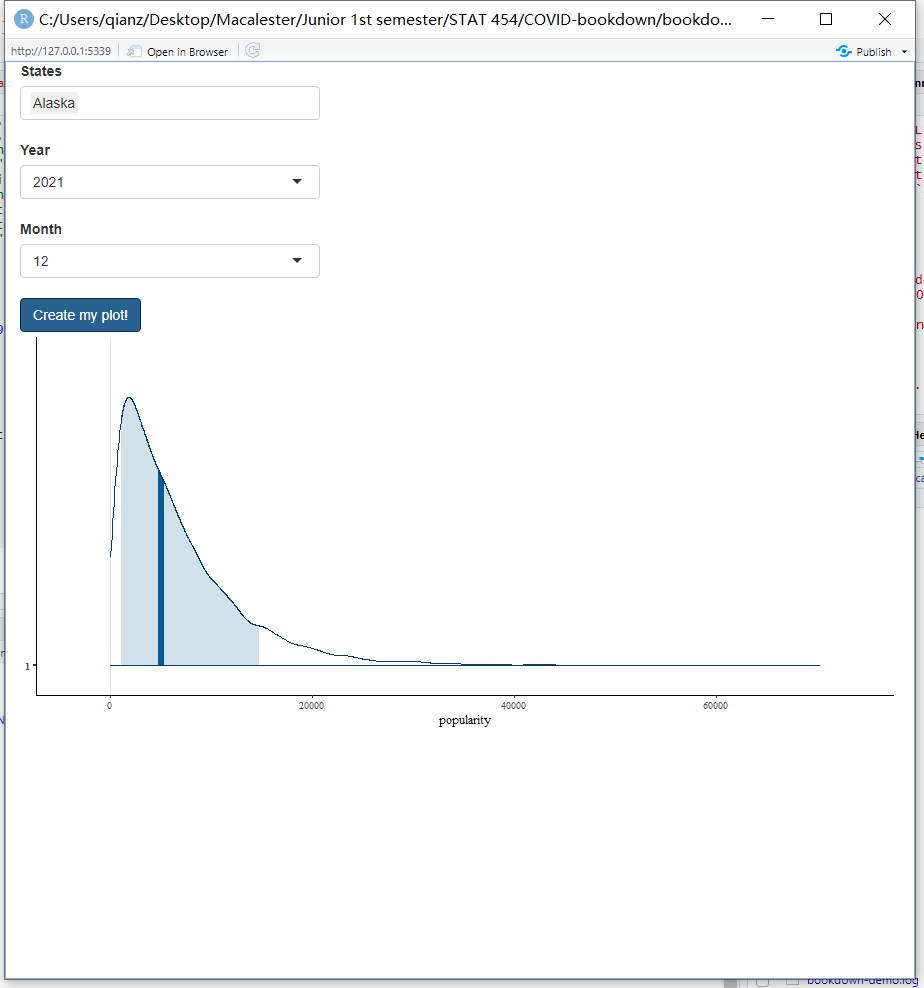
\includegraphics{baby_shinyapp.png}

\begin{enumerate}
\def\labelenumi{\arabic{enumi}.}
\tightlist
\item
  New York Time. (n.d.). Retrieved December 3, 2021, from \url{https://raw.githubusercontent.com/nytimes/covid-19-data/master/us-states.csv}.
\end{enumerate}

  \bibliography{book.bib,packages.bib}

\end{document}
